\documentclass[a4paper]{article}
\usepackage[T1]{fontenc}			% pacchetto per \chapter
\usepackage[italian]{babel}
\usepackage[italian]{isodate}  		% formato delle date in italiano
\usepackage{graphicx}				% gestione delle immagini
\usepackage{amsfonts}
\usepackage{booktabs}				% tabelle di qualità superiore
\usepackage{amsmath}				% pacchetto matematica
\usepackage{mathtools}				% per sottolineare sotto le equazioni
\usepackage{stmaryrd} 				% per '\llbracket' e '\rrbracket'
\usepackage{amsthm}					% teoremi migliorati
\usepackage{enumitem}				% gestione delle liste
\usepackage{pifont}					% pacchetto con elenchi carini
\usepackage{enumitem}				% pacchetto per elenchi con lettere dell'alfabeto
\usepackage{cancel}					% per cancellare delle espressioni matematiche
\usepackage{caption}				% caption personalizzati
\usepackage[]{mdframed}				% box per il testo
\usepackage{multirow}				% più linee in una tabella
\usepackage{gensymb}				% simbolo di degree


% draw a frame around given text
\newcommand{\framedtext}[1]{%
\par%
\noindent\fbox{%
    \parbox{\dimexpr\linewidth-2\fboxsep-2\fboxrule}{#1}%
}%
}



\usepackage[x11names]{xcolor}		% pacchetto colori RGB
% Link ipertestuali per l'indice
\usepackage{xcolor}
\usepackage[linkcolor=black, citecolor=blue, urlcolor=cyan]{hyperref}
\hypersetup{
	colorlinks=true
}

\usepackage{tikz}
\newcommand{\MyTikzmark}[2]{%
	\tikz[overlay,remember picture,baseline] \node [anchor=base] (#1) {#2};%
}
\newcommand{\DrawVLine}[3][]{%
	\begin{tikzpicture}[overlay,remember picture]
		\draw[shorten <=0.3ex, #1] (#2.north) -- (#3.south);
	\end{tikzpicture}
}
\newcommand{\DrawHLine}[3][]{%
	\begin{tikzpicture}[overlay,remember picture]
		\draw[shorten <=0.2em, #1] (#2.west) -- (#3.east);
	\end{tikzpicture}
}


%\usepackage{showframe}				% visualizzazione bordi
%\usepackage{showkeys}				% visualizzazione etichetta

\newtheorem{theorem}{\textcolor{Red3}{\underline{Teorema}}}
\newtheorem{lemma}{Lemma}
\renewcommand{\qedsymbol}{QED}
\newcommand{\exec}[1]{\llbracket #1\:\rrbracket}
\newcommand{\dquotes}[1]{``#1''}
\newcommand{\longline}{\noindent\rule{\textwidth}{0.4pt}}
\newcommand{\circledtext}[1]{\raisebox{.5pt}{\textcircled{\raisebox{-.9pt}{#1}}}}

\newenvironment{rowequmat}[1]{\left(\array{@{}#1@{}}}{\endarray\right)}
\newenvironment{rowequmatbra}[1]{\left[\array{@{}#1@{}}}{\endarray\right]}

\begin{document}
	\author{VR443470}
	\title{Guida agli Esami di Analisi II}
	\date{\printdayoff\today}
	\maketitle

	\newpage

	% indice
	\tableofcontents

	\newpage

	\section{Esercizio 1 - Problema di Cauchy}

	\subsection{Problema di Cauchy - Soluzione}

	Il primo esercizio è sempre uguale e riguarda il problema di Cauchy. Un esempio di testo tratto dal tema d'esame del 25/06/2021: \textcolor{Green4}{\textbf{\emph{Si trovi una soluzione locale del seguente problema di Cauchy e si determini l'intervallo massimale in cui tale soluzione è definita.}}}
	\begin{equation*}
		\begin{cases}
			y' + \dfrac{y^{3}}{x^{2} + 1} = 0 \\
			\\
			y\left(0\right) = 1
		\end{cases}
	\end{equation*}
	Il \textbf{primo passo} è esplicitare la derivata, per cui:
	\begin{equation*}
		\begin{cases}
			y' + \dfrac{y^{3}}{x^{2} + 1} = 0 \\
			\\
			y\left(0\right) = 1
		\end{cases}
		\longrightarrow
		\begin{cases}
			y' = -\dfrac{y^{3}}{x^{2} + 1} \\
			\\
			y\left(0\right) = 1
		\end{cases}
	\end{equation*}
	Il \textbf{secondo passo} è risolvere l'integrale per ciascuna parte:
	\begin{equation*}
		\begin{array}{rll}
			&\rightarrow& \displaystyle\int-\dfrac{y^{3}}{x^{2} + 1} \: \mathrm{d}x \\
			\\
			&\downarrow& y^{3}\text{ è costante, quindi si porta fuori dall'integrale} \\
			\\
			&\rightarrow& -y^{3} \cdot \displaystyle\int\dfrac{1}{x^{2} + 1} \: \mathrm{d}x \\
			\\
			&\downarrow& \text{l'integrale corrisponde all'arcotangente: } \int\frac{1}{x^{2} + a^{2}} \: dx = \frac{1}{a} \cdot \arctan\left(\frac{x}{a}\right) \\
			\\
			-\displaystyle\int \dfrac{1}{y^{3}} \: \mathrm{d}y &=& \dfrac{1}{1} \cdot \arctan\left(\dfrac{x}{1}\right) \\
			\\
			&\downarrow& \text{risoluzione dell'integrale a sinistra} \\
			\\
			\dfrac{1}{2y^{2}} &=& \arctan\left(x\right) \\
			\\
			&\downarrow& \text{si somma la costante }c\\
			\\
			\dfrac{1}{2y^{2}} &=& \arctan\left(x\right) + c
		\end{array}
	\end{equation*}
	Il risultato rappresenta la famiglia delle soluzioni delle funzioni $y$, chiamata anche \emph{soluzione generale}.\newpage

	\noindent
	Il \textbf{terzo passo} è sostituire la condizione iniziale all'interno della soluzione e calcolare il valore della costante $c$:
	\begin{equation*}
		\begin{array}{rll}
			\text{Condizione iniziale} &\longrightarrow& y\left(0\right) = 1 \\ [1em]
			\text{Sostituzione nella soluzione generale} &\longrightarrow& \dfrac{1}{2 \cdot 1^{2}} = \arctan\left(0\right) + c
		\end{array}
	\end{equation*}
	Quindi il valore di $c = \dfrac{1}{2}$.\newline

	\noindent
	Il \textbf{quarto e ultimo passo} riguarda \underline{l'intervallo massimale}. Per trovarlo, è necessario prendere in considerazione la soluzione generale trovata al punto 2:
	\begin{equation*}
		\dfrac{1}{2y^{2}} = \arctan\left(x\right) + c
	\end{equation*}
	Sostituire il valore $c$ con la soluzione trovata, nel nostro caso $\frac{1}{2}$:
	\begin{equation*}
		\dfrac{1}{2y^{2}} = \arctan\left(x\right) + \dfrac{1}{2}
	\end{equation*}
	Esplicitando la $y$, si ottiene:
	\begin{equation*}
		\begin{array}{rcl}
			\dfrac{1}{y^{2}} &=& 2 \cdot \arctan\left(x\right) + 1 \\ [1.5em]
			y^{-2} &=& \dfrac{1}{2 \arctan\left(x\right) + 1} \\ [1.5em]
			y &=& \dfrac{1}{\sqrt{2 \arctan\left(x\right) + 1}}
		\end{array}
	\end{equation*}
	A questo punto, si afferma che il problema ha soluzione solo se:
	\begin{equation*}
		\arctan\left(x\right) + \dfrac{1}{2} > 0
	\end{equation*}
	Si esplicita la $x$ ricordando che $\tan^{-1}\left(x\right) = y$ è l'inversa di $x = \tan\left(y\right)$:
	\begin{equation*}
		\begin{array}{rcl}
			\arctan\left(x\right) + \dfrac{1}{2} &>& 0 \\
			\arctan\left(x\right) &>& -\dfrac{1}{2} \\ [1em]
			x &>& \tan\left(-\dfrac{1}{2}\right) \\ [1em]
			x &>& -\tan\left(\dfrac{1}{2}\right)
		\end{array}
	\end{equation*}\newpage

	\subsection{Riepilogo dei passaggi}

	\begin{table}[!htp]
		\centering
		\begin{tabular}{@{} l p{23em} @{}}
			\toprule
			\textbf{Passaggio} & \textbf{Descrizione} \\
			\midrule
			1°	& Esplicitare la $y'$ a sinistra. Può capitare, talvolta, che la $y'$ sia in compagnia. In questo caso, eseguire alcune manipolazioni algebriche così da isolarla. \\ [.5em]
			2°	& Calcolare l'integrale a destra dell'uguale. Per farlo, si esegue l'integrale rispetto a $x$ così da portare fuori la costante $y$. \\ [.5em]
			3°	& Portare la $y$ a sinistra dell'uguale, ricordando di \underline{non} cambiare segno, ma di moltiplicarla per $-1$, ovverosia di ribaltare numeratore e denominatore. \\ [.5em]
			4°	& Eseguire l'integrale della parte a sinistra dell'uguale rispetto a $y$ (a questo punto a destra si dovrebbe avere il risultato dell'integrale rispetto ad $x$). \\ [.5em]
			5°	& Si aggiunge la costante $+ c$, si applica la condizione iniziale e si esplicita la costante $c$. Infatti, applicando la condizione iniziale, l'unica incognita che rimane è $c$, per cui dovrebbe essere immediato ottenerla. \\ [.5em]
			6°  & Adesso è necessario ottenere l'intervallo massimo. Si sostituisce la $c$ ottenuta al punto $5$ nella soluzione dei due integrali dove è stata inserita la costante $+ c$ (alla fine del passo $4$). \\ [.5em]
			7°	& Con la sostituzione della costante $c$, si esplicita la $y$ eseguendo alcune operazioni algebriche. \\ [.5em]
			8°  & Si ottiene la/le condizione/i di esistenza del valore che assume $y$ e si esplicita la $x$. \\
			\bottomrule
		\end{tabular}
	\end{table}\newpage

	\subsection{Vari esercizi d'esame}

	\subsubsection{Esame del 10/07/2023 - Gruppo A}

	\textcolor{Green4}{\textbf{\emph{Determinare la soluzione del seguente problema di Cauchy}}}
	\begin{equation*}
		\begin{cases}
			y' = \dfrac{x^{2} e^{-y^{2}}}{y} \\
			y\left(0\right) = 1
		\end{cases}
	\end{equation*}
	\textcolor{Green4}{\textbf{\emph{e indicare il più ampio \underline{intervallo} su cui tale soluzione è definita.}}}\newline
		
	\noindent
	Il primo passo è esplicitare la derivata. Tuttavia, in questo caso è già esplicitata. Si prosegue con il secondo passo che è risolvere l'integrale per ciascuna parte:
	\begin{equation*}
		\begin{array}{rcl}
			&\rightarrow& \displaystyle\int\dfrac{x^{2} e^{-y^{2}}}{y} \: \mathrm{d}x \hspace{1em} y \ne 0 \\
			\\
			&\rightarrow& \displaystyle\int x^{2} \cdot \dfrac{e^{-y^{2}}}{y} \: \mathrm{d}x \\
			\\
			&\rightarrow& \dfrac{e^{-y^{2}}}{y} \cdot \displaystyle\int x^{2} \: \mathrm{d}x \\
			\\
			\displaystyle\int\dfrac{y}{e^{-y^{2}}} \: \mathrm{d}y &=& \displaystyle\int x^{2} \: \mathrm{d}x \\
			\\
			\displaystyle\int y \cdot \dfrac{1}{e^{-y^{2}}} &=& \dfrac{x^{3}}{3} \\
			\\
			\displaystyle\int y \cdot e^{y^{2}} &=& \dfrac{x^{3}}{3} \\
			\\
			&\downarrow& \text{integrale notevole del tipo } \displaystyle\int f'\left(x\right) \cdot e^{f\left(x\right)} \: \mathrm{d}x \text{ quindi si aggiunge }\times 2 \\
			\\
			\displaystyle\int 2 y \cdot e^{y^{2}} &=& 2 \cdot \dfrac{x^{3}}{3} \\
			\\
			e^{y^{2}} &=& \dfrac{2x^{3}}{3} + c
		\end{array}
	\end{equation*}
	Il terzo passo è imporre la condizione iniziale:
	\begin{equation*}
		\begin{array}{rcl}
			\text{Condizione iniziale} 	&\longrightarrow& y\left(0\right) = 1 \\
			\\
			\text{Sostituzione}			&\longrightarrow& e^{1^{2}} = \dfrac{2 \cdot 0^{3}}{3} + c
		\end{array}
	\end{equation*}
	Quindi il valore di $c = e$. Infine, l'esercizio si conclude cercando l'intervallo massimale. Esso è ottenibile prendendo la soluzione generale e sostituendo al posto della costante $c$, il valore trovato:
	\begin{equation*}
		\begin{array}{rcl}
			e^{y^{2}} &=& \dfrac{2x^{3}}{3} + c \\
			\\
			e^{y^{2}} &=& \dfrac{2x^{3}}{3} + e \\
			\\
			y^{2} &=& \ln\left(\dfrac{2x^{3}}{3} + e\right) \\
			\\
			y &=& \sqrt{\ln\left(\dfrac{2x^{3}}{3} + e\right)} \\
		\end{array}
	\end{equation*}
	Inoltre, grazie all'esplicitazione della $y$, adesso è possibile ottenere le condizioni di esistenza:
	\begin{itemize}
		\item Per il logaritmo $\dfrac{2x^{3}}{3} + e > 0$
		\item Per la radice $\ln\left(\dfrac{2x^{3}}{3} + e\right) > 0$
	\end{itemize}
	Dato che la prima condizione di esistenza è contenuta nella seconda, allora quest'ultima implica la prima. Inoltre, nella seconda condizione è possibile rimuovere il logaritmo enunciando la proprietà dei logaritmi: un logaritmo è maggiore di zero se il suo argomento è maggiore di $1$. In questo caso, l'argomento è $\dfrac{2x^{3}}{3} + e$ per cui si pone maggiore di uno:
	\begin{equation*}
		\dfrac{2x^{3}}{3} + e > 1
	\end{equation*}
	Si procede esplicitando la $x$:
	\begin{equation*}
		\begin{array}{rcl}
			x^{3} &>& \left(1-e\right) \cdot \dfrac{3}{2} \\ [.5em]
			x &>& \sqrt[3]{\dfrac{3}{2} \cdot \left(1-e\right)}
		\end{array}
	\end{equation*}
	Quindi, l'intervallo massimo parte dalla condizione esplicitata qua sopra e arriva fino ad $\infty$:
	\begin{equation*}
		\left] \sqrt[3]{\dfrac{3}{2} \cdot \left(1-e\right)}, \infty \right[
	\end{equation*}\newpage

	\section{Esercizio 2 - Problema di Cauchy con variabile $t$ e $y''$}

	\subsection{Risoluzione del problema di cauchy con $y''$}

	Il secondo esercizio è un problema di Cauchy un po' più complesso poiché utilizza il metodo di somiglianza\footnote{\href{https://youtu.be/Ij2V7cj_lh8}{Link utile}}. Un esempio di testo estratto dal tema d'esame del 25/06/2021: \textcolor{Green4}{\textbf{\emph{Si trovi la soluzione del seguente problema di Cauchy definita per ogni $t \in \mathbb{R}$:}}}
	\begin{equation*}
		\begin{cases}
			y'' - y' = 1 - 2t \\
			y\left(0\right) = 0 \\
			y'\left(0\right) = 2
		\end{cases}
	\end{equation*}
	Il \textbf{primo passo} è scrivere l'equazione caratteristica che corrisponde sempre alla prima equazione:
	\begin{equation*}
		y'' - y' = 1 - 2t \longrightarrow \lambda^{2} - \lambda = 0
	\end{equation*}
	L'equazione caratteristica deve essere posta uguale a zero.\newline

	\noindent
	Il \textbf{secondo passo} è risolvere l'equazione caratteristica così da avere le soluzioni reali distinte:
	\begin{equation*}
		\lambda_{1} = 0, \lambda_{2} = 1
	\end{equation*}
	Il \textbf{terzo passo} è scrivere l'integrale generale $y\left(t\right)$ indicando con $y_{P}\left(t\right)$ una soluzione particolare dell'equazione completa:
	\begin{equation*}
		y\left(t\right) = y_{P}\left(t\right) + c_{1}e^{0t} + c_{2}e^{1t} \hspace{1em} c_{1}, c_{2} \in \mathbb{R}
	\end{equation*}
	Escludendo questo esercizio, in generale l'integrale generale è sempre così. Gli unici termini che cambiano sono le $e$ che hanno come esponente la soluzione dell'equazione moltiplicata per $t$.\newline

	\noindent
	Dato che una soluzione dell'equazione caratteristica è $0$ e $1-2t$ è un polinomio di primo grado, $y_{P}\left(t\right)$ sarà:
	\begin{equation*}
		y_{P}\left(t\right) = \left(at + b\right)t^{1} = at^{2} + bt
	\end{equation*}
	Dove l'esponente 1 indica quante volte si ripete il valore zero.
	\begin{mdframed}
		\textbf{\underline{N.B.}} Esistono diverse casistiche e ciascuno cambia l'equazione della soluzione particolare:
		\begin{itemize}
			\item \textbf{Polinomio di secondo grado}. In questo caso si scrive un'equazione di secondo grado generale
			\begin{equation*}
				\begin{array}{rcl}
					\text{Esercizio di esempio:} &\longrightarrow& y''+3y'+2y = 2x^{2} -1 \\ [1em]
					\text{Soluzione particolare:} &\longrightarrow& y_{P}\left(x\right) = ax^{2} + bx + c
				\end{array}
			\end{equation*}\newpage

			\item \textbf{Polinomio con un esponenziale}. In questo caso si scrive un'equazione contenente l'esponenziale per un valore generico:
			\begin{equation*}
				\begin{array}{rcl}
					\text{Esercizio di esempio:} &\longrightarrow& y''+y'-2y = 3e^{-x} \\ [1em]
					\text{Soluzione particolare:} &\longrightarrow& y_{P}\left(x\right) = ae^{-x}
				\end{array}
			\end{equation*}

			\item \textbf{Polinomio di primo grado}. In questo caso si scrive un'equazione di primo grado generale:
			\begin{equation*}
				\begin{array}{rcl}
					\text{Esercizio di esempio:} &\longrightarrow& y''+y'-2y = x+2 \\ [1em]
					\text{Soluzione particolare:} &\longrightarrow& y_{P}\left(x\right) = ax + b
				\end{array}
			\end{equation*}

			\item \textbf{Soluzione dell'equazione caratteristica che compare nel polinomio}. In questo caso, è necessario aggiungere la $x$ elevandola al numero di ripetizioni nel polinomio:
			\begin{equation*}
				\begin{array}{rcl}
					\text{Esercizio di esempio:} &\longrightarrow& y''+3y'+2y = 3e^{x} \\ [1em]
					\text{Soluzione particolare:} &\longrightarrow& y_{P}\left(x\right) = a \cdot x^{1} \cdot e^{x}
				\end{array}
			\end{equation*}
			
			\item \textbf{Soluzione dell'equazione caratteristica uguale a zero ($\lambda = 0$)}. In questo caso, è necessario aggiungere una $x$ elevandola al numero di volte in cui $\lambda = 0$ annulla l'equazione (molteplicità algebrica):
			\begin{equation*}
				\begin{array}{rcl}
					\text{Esercizio di esempio:} &\longrightarrow& y''+y' = x+2 \\ [1em]
					\text{Soluzione particolare:} &\longrightarrow& y_{P}\left(x\right) = \left(ax+b\right) x^{1}
				\end{array}
			\end{equation*}

			\item \textbf{Soluzioni dell'equazione caratteristica uguali tra di loro ($\lambda_{1} = \lambda_{2}$)}. In questo caso, è necessario aggiungere una $x$ alla soluzione generale e non alla soluzione particolare!
			\begin{equation*}
				\begin{array}{rcl}
					\text{Esercizio di esempio:} &\longrightarrow& y'' - 2y' + y = \left(x-1\right)^{2} \\ [1em]
					\text{Soluzione particolare:} &\longrightarrow& y\left(x\right) = y_{P}\left(x\right) + c_{1} e^{x} + c_{2} e^{x} \cdot x
				\end{array}
			\end{equation*}

			\item \textbf{Coseno o seno}. In questo caso, è necessario scrivere entrambe le funzioni trigonometriche:
			\begin{equation*}
				\begin{array}{rcl}
					\text{Esercizio di esempio:} &\longrightarrow& y''+y' = \cos\left(2x\right) \\ [1em]
					\text{Soluzione particolare:} &\longrightarrow& y_{P}\left(x\right) = a \cos\left(2x\right) + b \sin\left(2x\right)
				\end{array}
			\end{equation*}
		\end{itemize}
	\end{mdframed}

	\noindent
	Il \textbf{quarto passo} è eseguire la derivata prima e seconda della soluzione particolare:
	\begin{equation*}
		\begin{array}{rcl}
			y_{P}\left(t\right) &=& at^{2} + bt \\
			y_{P}'\left(t\right) &=& 2at + b\\
			y_{P}''\left(t\right) &=& 2a
		\end{array}
	\end{equation*}\newpage

	\noindent
	Il \textbf{quinto passo} è sostituire le derivate trovate nel problema iniziale, ovvero in $y''-y'$, e risolvere il sistema equivalente:
	\begin{equation*}
		\begin{array}{rcl}
			y'' - y' &=& 1 - 2t \\
			\left(2a\right) - \left(2at+b\right) &=& 1-2t \\
			2a -2at -b &=& 1-2t \\
			\left(-2a\right)t + \left(2a-b\right) &=& \left(-2\right)t + \left(1\right) \\
			\\
			\begin{cases}
				-2a = -2 \\
				2a - b = 1
			\end{cases} &\longrightarrow&
			\begin{cases}
				a = 1 \\
				b = 1
			\end{cases}
		\end{array}
	\end{equation*}
	Il \textbf{sesto passo} è sostituire i valori trovati nella soluzione particolare:
	\begin{equation*}
		y_{P}\left(t\right) = at^{2} + bt \rightarrow y_{P}\left(t\right) = 1 \cdot t^{2} + 1 \cdot t = t^{2} + t
	\end{equation*}
	Il \textbf{settimo passo} è riscrivere l'integrale generale $y\left(t\right)$ con la soluzione particolare:
	\begin{equation*}
		y\left(t\right) = t^{2} + t + c_{1} + c_{2}e^{1t}
	\end{equation*}
	Ed eseguire la derivata prima di tale equazione:
	\begin{equation*}
		\begin{array}{rcl}
			y'\left(t\right) &=& \dfrac{\mathrm{d}}{\mathrm{d}t} t^{2} + t + c_{1} + c_{2}e^{t} \\ [1em]
			y'\left(t\right) &=& 2t + 1 + c_{2}e^{t}
		\end{array}
	\end{equation*}
	L'\textbf{ottavo passo} conclude l'esercizio. Si esegue una sostituzione delle condizioni del problema nell'integrale generale e nella sua derivata così da trovare le costanti $c_{1}$ e $c_{2}$:
	\begin{equation*}
		\begin{cases}
			y\left(0\right) = 0 	&\longrightarrow 0^{2} + 0 + c_{1} + c_{2}e^{0} = 0 \\
			y'\left(0\right) = 2 	&\longrightarrow 2 \cdot 0 + 1 + c_{2}e^{0} = 2
		\end{cases}
		\longrightarrow
		\begin{cases}
			c_{1} + c_{2} = 0 \\
			c_{2} = 1
		\end{cases}
		\longrightarrow
		\begin{cases}
			c_{1} = -1 \\
			c_{2} = 1
		\end{cases}
	\end{equation*}
	Infine, si scrive la soluzione del problema di Cauchy sostituendo le costanti nell'integrale generale:
	\begin{equation*}
		y\left(t\right) = t^{2} + t -1 + e^{t}
	\end{equation*}\newpage

	\subsection{Vari esercizi d'esame}

	\subsubsection{Esame del 10/07/2023 - Gruppo A}

	\textcolor{Green4}{\textbf{\emph{Si trovi la soluzione del seguente problema di Cauchy, definita per ogni $t \in \mathbb{R}$:}}}
	\begin{equation*}
		\begin{cases}
			y''\left(t\right) - 2y'\left(t\right) + y\left(t\right) = \left(t-1\right)^{2} \\
			y\left(0\right) = 1 \\
			y'\left(0\right) = 0
		\end{cases}
	\end{equation*}
	Il primo semplice passaggio è riscrivere l'equazione caratteristica corrispondente alla prima equazione e ottenere le relative soluzioni.
	\begin{equation*}
		\begin{array}{rcl}
			y''\left(t\right) - 2y'\left(t\right) + y\left(t\right) &=& 0 \\ [.5em]
			\lambda^{2} - 2\lambda + 1 &=& 0 \\
			&\downarrow& \\
			\lambda_{1} = \lambda_{2} &=& 1
		\end{array}
	\end{equation*}
	Le soluzioni ottenute vengono inserite nella soluzione generale, ricordando di aggiungere una moltiplicazione per $t$ poiché le soluzioni $lambda$ sono uguali:
	\begin{equation*}
		y\left(t\right) = y_{P}\left(t\right) + c_{1} e^{1 \cdot t} + c_{2} e^{1 \cdot t} \cdot t
	\end{equation*}
	Si risolve con il metodo di somiglianza, quindi si scrive la soluzione particolare:
	\begin{equation*}
		\begin{array}{rcl}
			\left(t-1\right)^{2} &=& t^{2} -2t + 1 \\
			y_{P}\left(t\right) &=& at^{2} + bt + c
		\end{array}
	\end{equation*}
	Si eseguono le derivate prima e seconda poiché è necessario sostituirle nell'equazione originale:
	\begin{equation*}
		\begin{array}{rcl}
			y_{P}\left(t\right) &=& at^{2} + bt + c \\ [.3em]
			y_{P}'\left(t\right) &=& 2at + b \\ [.3em]
			y_{P}''\left(t\right) &=& 2a
		\end{array}
	\end{equation*}
	Sostituzione nell'equazione iniziale:
	\begin{equation*}
		\begin{array}{rcl}
			y''\left(t\right) - 2y'\left(t\right) + y\left(t\right) &=& \left(t-1\right)^{2} \\ [.5em]
			\left(2a\right) - 2\left(2at + b\right) + \left(at^{2} + bt + c\right) &=& t^{2} -2t + 1 \\ [.5em]
			2a - 4at - 2b + at^{2} + bt + c &=& t^{2} -2t + 1 \\ [.5em]
			\left(a\right)t^{2} + \left(-4a + b\right)t + \left(2a - 2b + c\right) &=& \left(1\right)t^{2} + \left(-2\right)t + \left(1\right)
		\end{array}
	\end{equation*}
	Si costruisce il sistema relativo:
	\begin{equation*}
		\begin{cases}
			a = 1 \\ 
			-4a + b = -2 \\
			2a - 2b + c = 1
		\end{cases}
		\longrightarrow
		\begin{cases}
			a = 1 \\
			b = 2 \\
			2 - 2b + c = 1
		\end{cases}
		\longrightarrow
		\begin{cases}
			a = 1 \\
			b = 2 \\
			c = 3
		\end{cases}
	\end{equation*}
	Si inseriscono i valori delle incognite nella soluzione particolare:
	\begin{equation*}
		y_{P}\left(t\right) = at^{2} + bt + c = t^{2} + 2t + 3
	\end{equation*}
	E si riscrive l'integrale generale:
	\begin{equation*}
		y\left(t\right) = t^{2} + 2t + 3 + c_{1} e^{t} + c_{2} e^{t} \cdot t
	\end{equation*}\newpage

	\noindent
	Adesso, si esegue la derivata parziale prima e si applicano le due condizioni iniziali rispetto $y$ e $y'$:
	\begin{equation*}
		\begin{array}{rcl}
			y\left(t\right) &=& t^{2} + 2t + 3 + c_{1} e^{t} + c_{2} e^{t} \cdot t \\ [.5em]
			y'\left(t\right) &=& 2t + 2 + c_{1} e^{t} + c_{2} e^{t} \cdot t + c_{2} e^{t}
		\end{array}
	\end{equation*}
	Applicazione condizioni iniziali:
	\begin{equation*}
		\begin{cases}
			1 = 0^{2} + 2 \cdot 0 + 3 + c_{1}e^{0} + c_{2}e^{0} \cdot 0 \\
			0 = 2 \cdot 0 + 2 + c_{1} e^{0} + c_{2}e^{0} \cdot 0 + c_{2}e^{0}
		\end{cases}
		\rightarrow
		\begin{cases}
			1 = 3 + c_{1} \\
			0 = 2 + c_{1} + c_{2}
		\end{cases}
		\rightarrow
		\begin{cases}
			-2 = c_{1} \\
			0 = c_{2}
		\end{cases}
	\end{equation*}
	Infine, si riscrive la soluzione del problema di Cauchy:
	\begin{equation*}
		y\left(t\right) = t^{2} + 2t + 3 -2e^{t}
	\end{equation*}

	\newpage

	\section{Esercizio 3 - Studio di funzione}

	\subsection{Tipologie di esercizio}

	\subsubsection{Rappresentare la funzione nel piano cartesiano}\label{par: rappresentare la funzione nel piano cartesiano}

	Un esercizio semplice che ad oggi viene fuso con altri esercizi, è quello della rappresentazione della funzione nel piano cartesiano. Si prenda in considerazione l'esame del 25/06/2021: \textcolor{Green4}{\textbf{\emph{Sia $D\subset\mathbb{R}^{2}$ il dominio naturale della funzione:}}
	\begin{equation*}
		f\left(x,y\right) = \sqrt{y-x^{2}}-\ln\left(4x-x^{2}-4y^{2}\right)
	\end{equation*}
	\textbf{\emph{Si rappresenti $D$ nel piano cartesiano.}}}\newline

	\noindent
	Il \textbf{primo passo} è rappresentare il dominio della funzione. In questo caso, è necessario affermare che l'espressione sotto radice sia maggiore/uguale di zero (per rimanere nei reali) e l'espressione del logaritmo sia strettamente maggiore di zero (con zero il logaritmo non ha soluzione):
	\begin{equation*}
		D = \left\{\left(x,y\right) \in \mathbb{R}^{2} \: : \: \left(y-x^{2} \ge 0\right) \land \left(4x-x^{2}-4y^{2} > 0\right)\right\}
	\end{equation*}
	\begin{mdframed}
		\textbf{\underline{N.B.}} Esistono diverse casistiche:
		\begin{itemize}
			\item \textbf{Frazione}:
			\begin{equation*}
				f\left(x,y\right) = \dfrac{\log\left(x+1\right)}{\sqrt{x^{2}+4y^{2}-1}}
			\end{equation*}
			Nonostante ci sia una radice quadrata, al denominatore non può esserci uno zero! Per cui, il dominio deve essere:
			\begin{equation*}
				D = \left\{\left(x,y\right) \in \mathbb{R}^{2} \: : \: \left(x+1 > 0\right) \land \left(x^{2} +4y^{2} -1 > 0\right)\right\}
			\end{equation*}

			\item \textbf{Radice quadrata e logaritmo annidato}:
			\begin{equation*}
				f\left(x,y\right) = y + \dfrac{1}{\sqrt{1 - \ln\left(y-x^{2}\right)}} - \ln\left(x\right)
			\end{equation*}
			In cui il suo dominio è:
			\begin{equation*}
				D = \left\{\left(x,y\right) \in \mathbb{R}^{2} \: : \: \left(y > x^{2}\right) \land \left(y < x^{2}\right)\right\}
			\end{equation*}
		\end{itemize}
	\end{mdframed}\newpage
	
	\noindent
	Il \textbf{secondo passo} è calcolare i punti appartenenti al dominio, così da poter rappresentare il grafico sul piano cartesiano. Per farlo, si prende ogni condizione presente nel dominio e si calcolano un po' di punti:
	\begin{table}[!htp]
		\begin{minipage}{.5\textwidth}
			\centering
			\begin{tabular}{@{} c | c @{}}
				\toprule
				$x$ & $y$ \\
				\midrule
				$0$	& $0$ 	\\
				$\pm1$ & $1$	\\
				$\pm2$	& $4$	\\
				\bottomrule
			\end{tabular}
			\caption*{Punti di $y-x^{2}$}
		\end{minipage}
		\begin{minipage}{.5\textwidth}
			\centering
			\begin{tabular}{@{} c | c @{}}
				\toprule
				$x$ & $y$ \\
				\midrule
				$0$	& $0$ \\
				$1$ & $\pm\frac{\sqrt{3}}{4}$	\\
				$2$ & $\pm 1$	\\
				\bottomrule
			\end{tabular}
			\caption*{Punti di $4x-x^{2}-4y^{2}$}
		\end{minipage}
	\end{table}
	\begin{figure}[!htp]
		\centering
		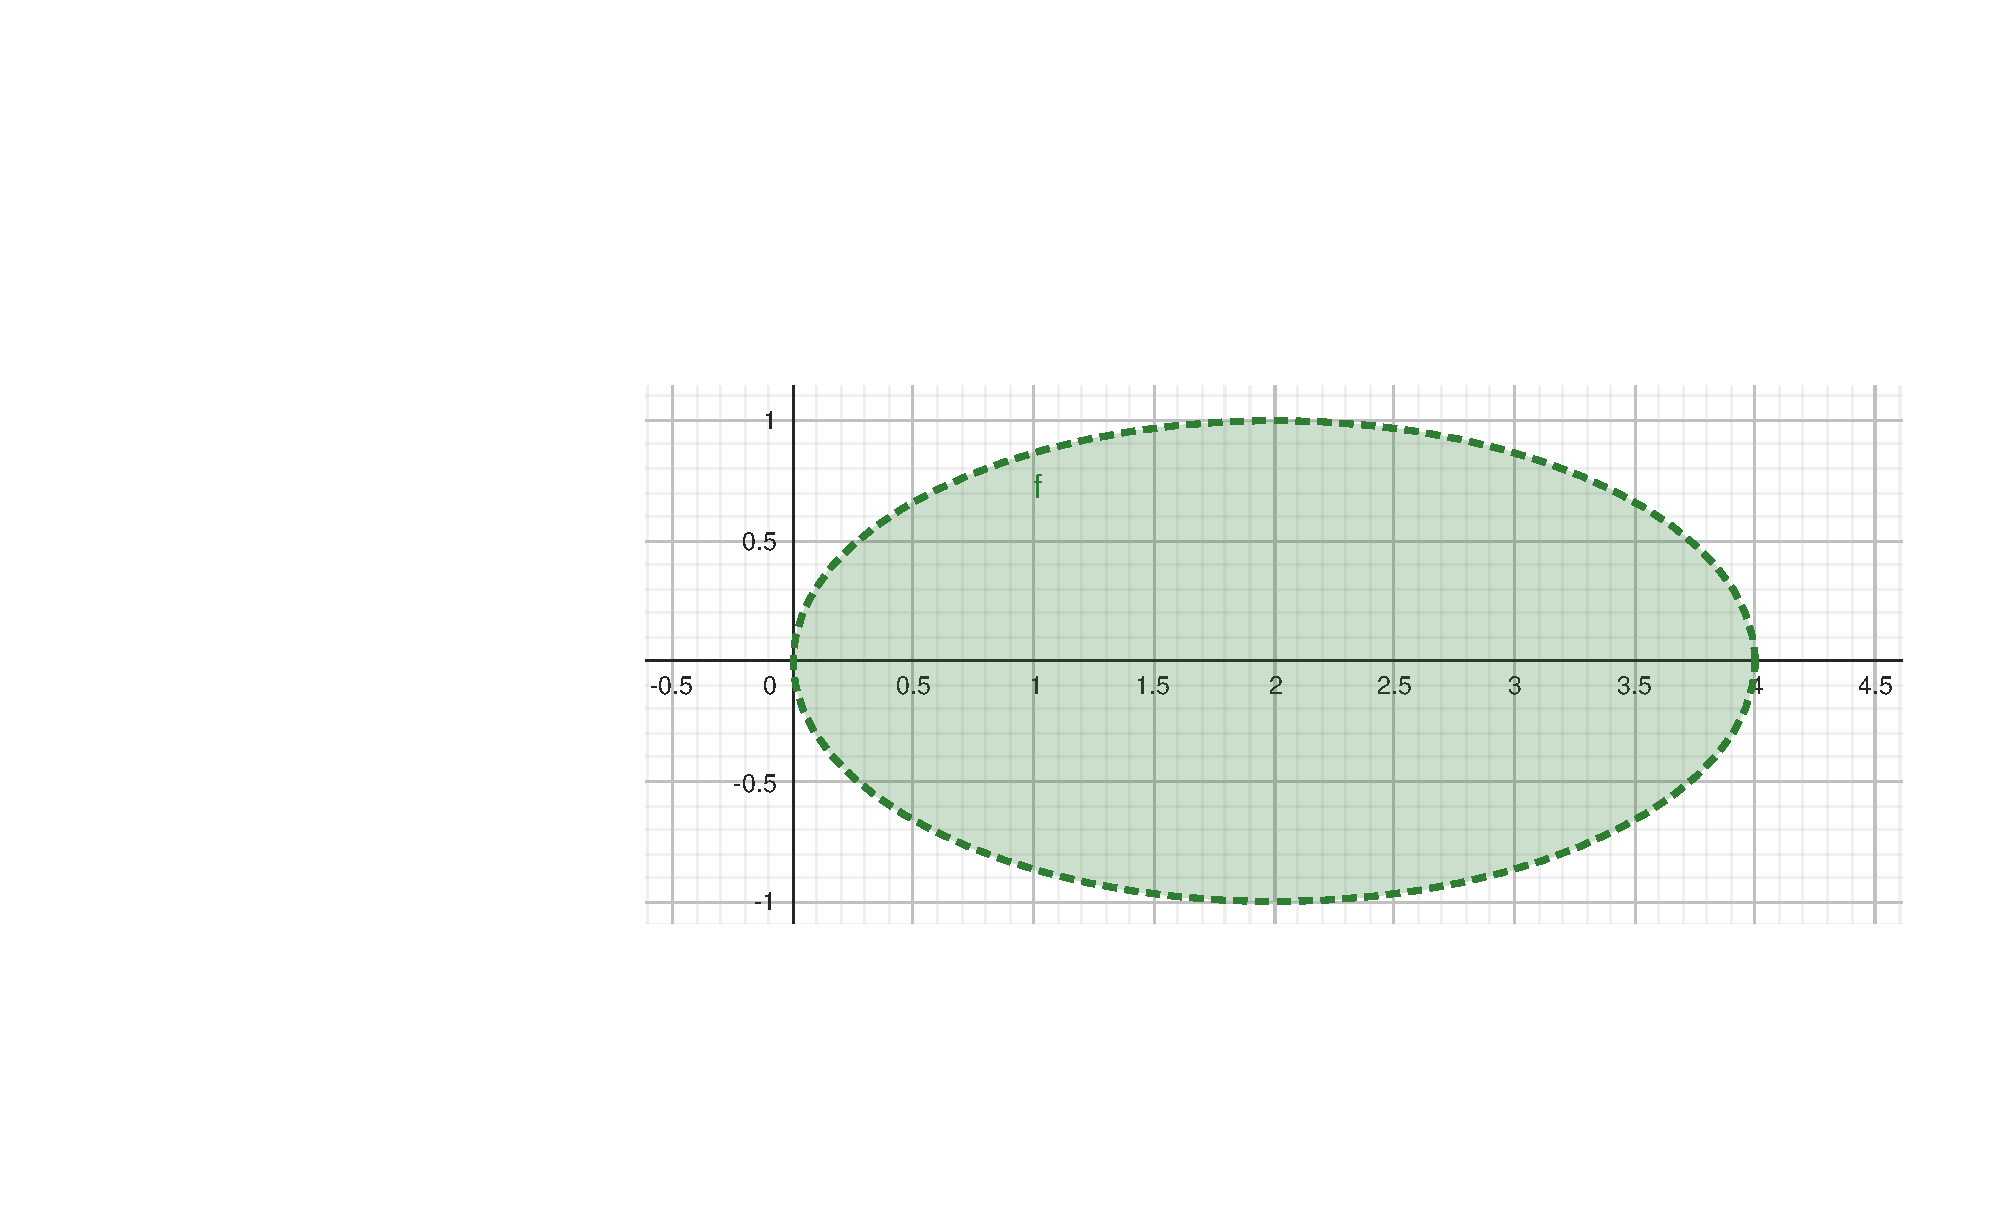
\includegraphics[width=.9\textwidth]{img/grafico-ex3-1.pdf}
		\caption*{Grafico $4x-x^{2}-4y^{2} > 0$.}
	\end{figure}

	\begin{figure}[!htp]
		\centering
		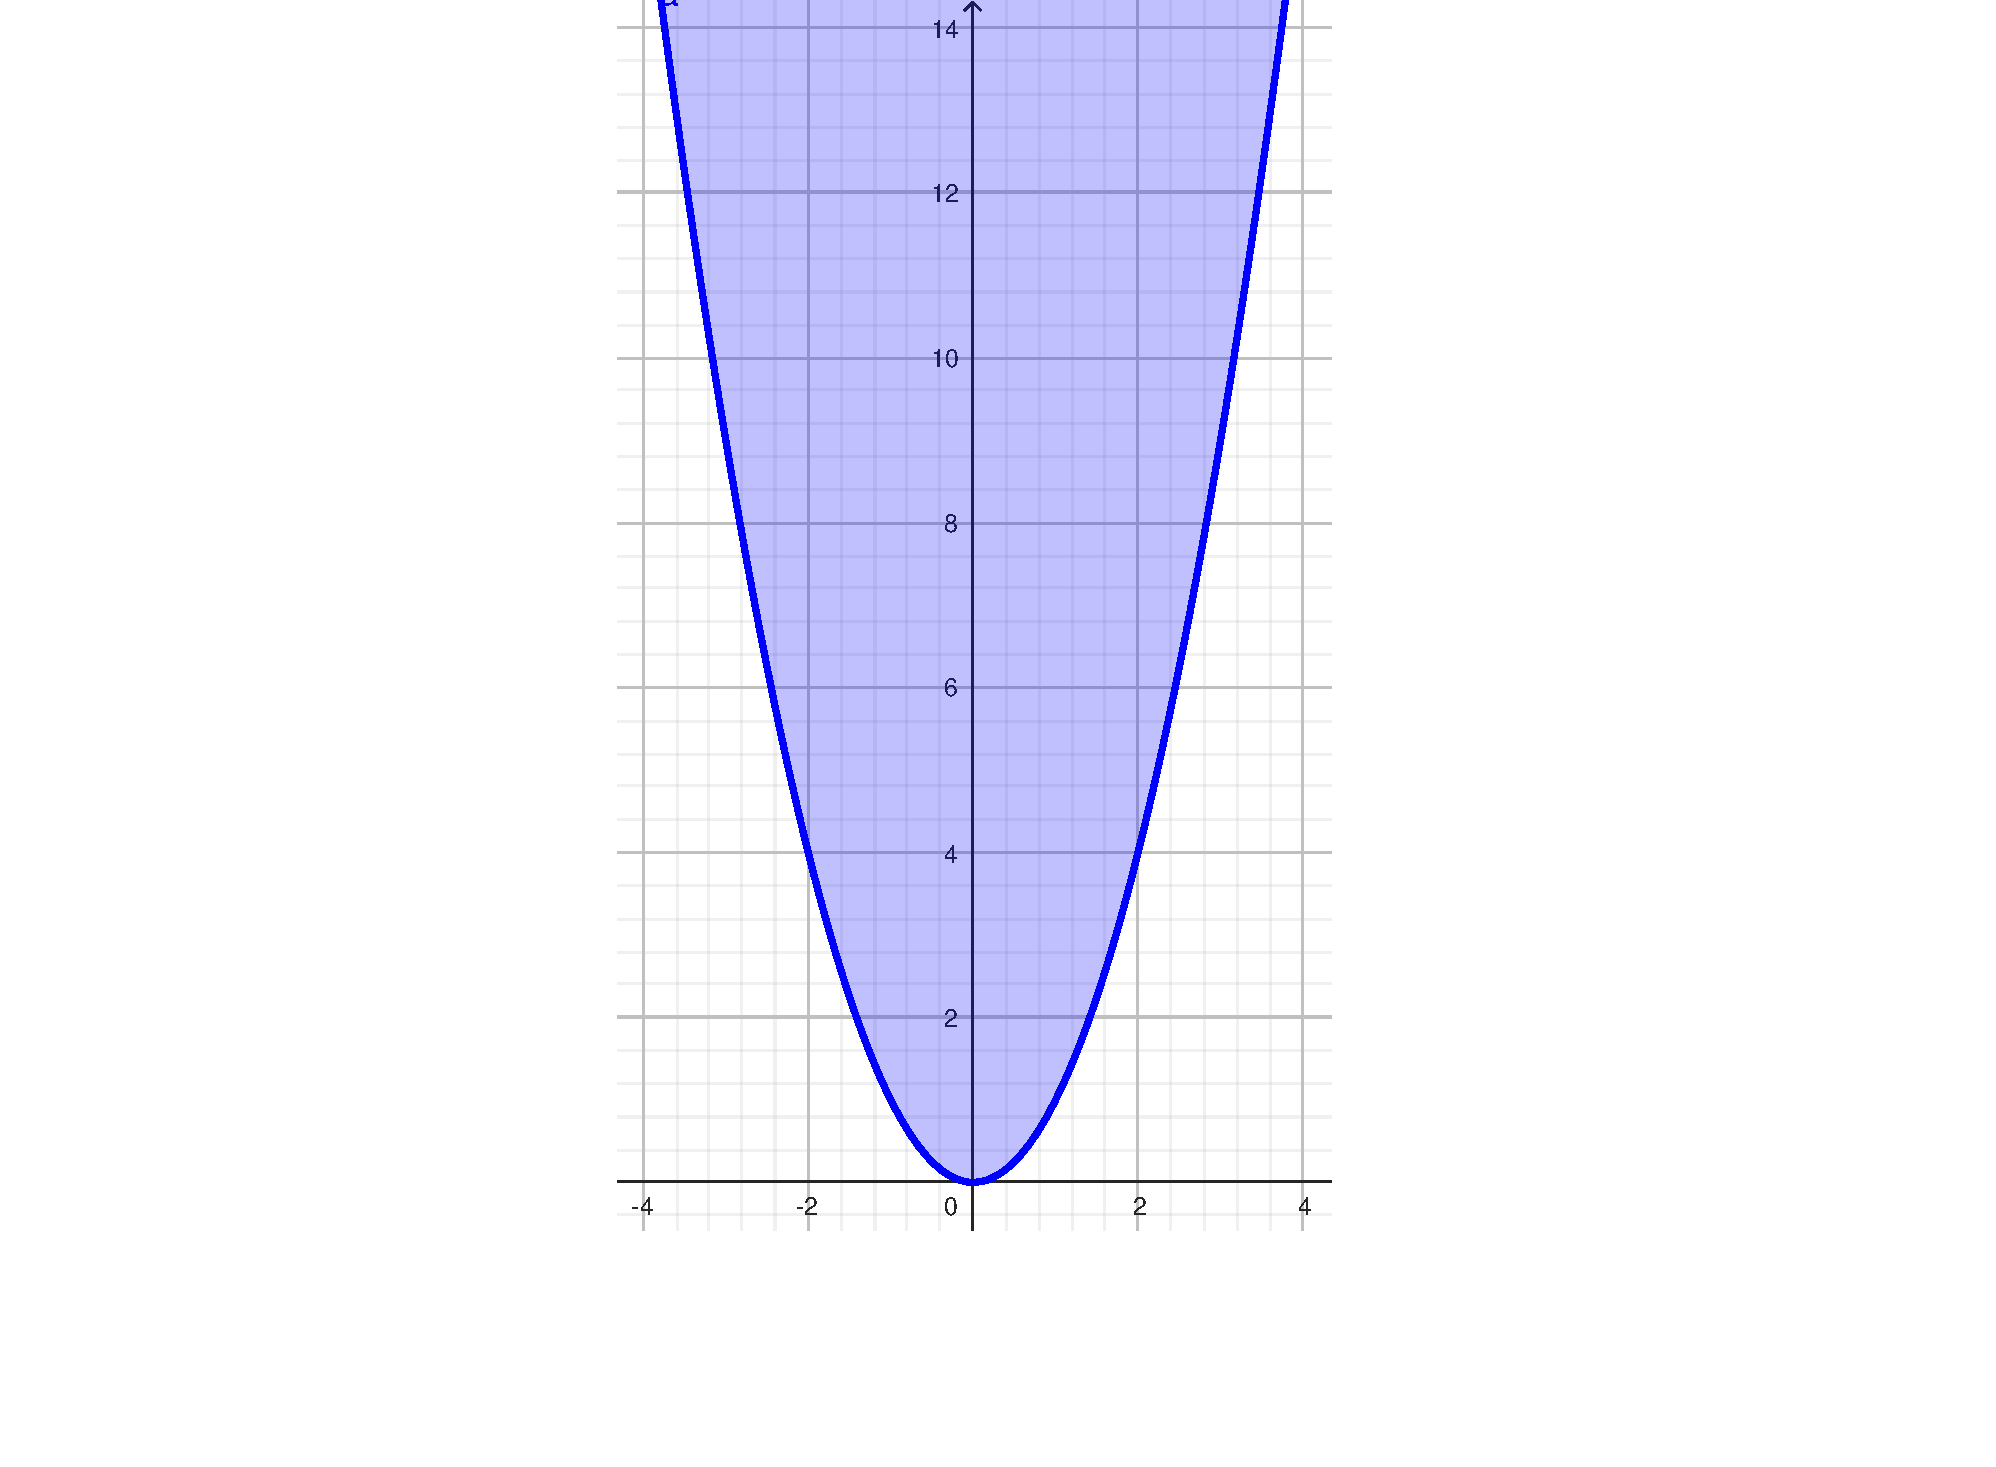
\includegraphics[width=.4\textwidth]{img/grafico-ex3-2.pdf}
		\caption*{Grafico $y-x^{2} \ge 0$.}
	\end{figure}\newpage
	
	\begin{figure}[!htp]
		\centering
		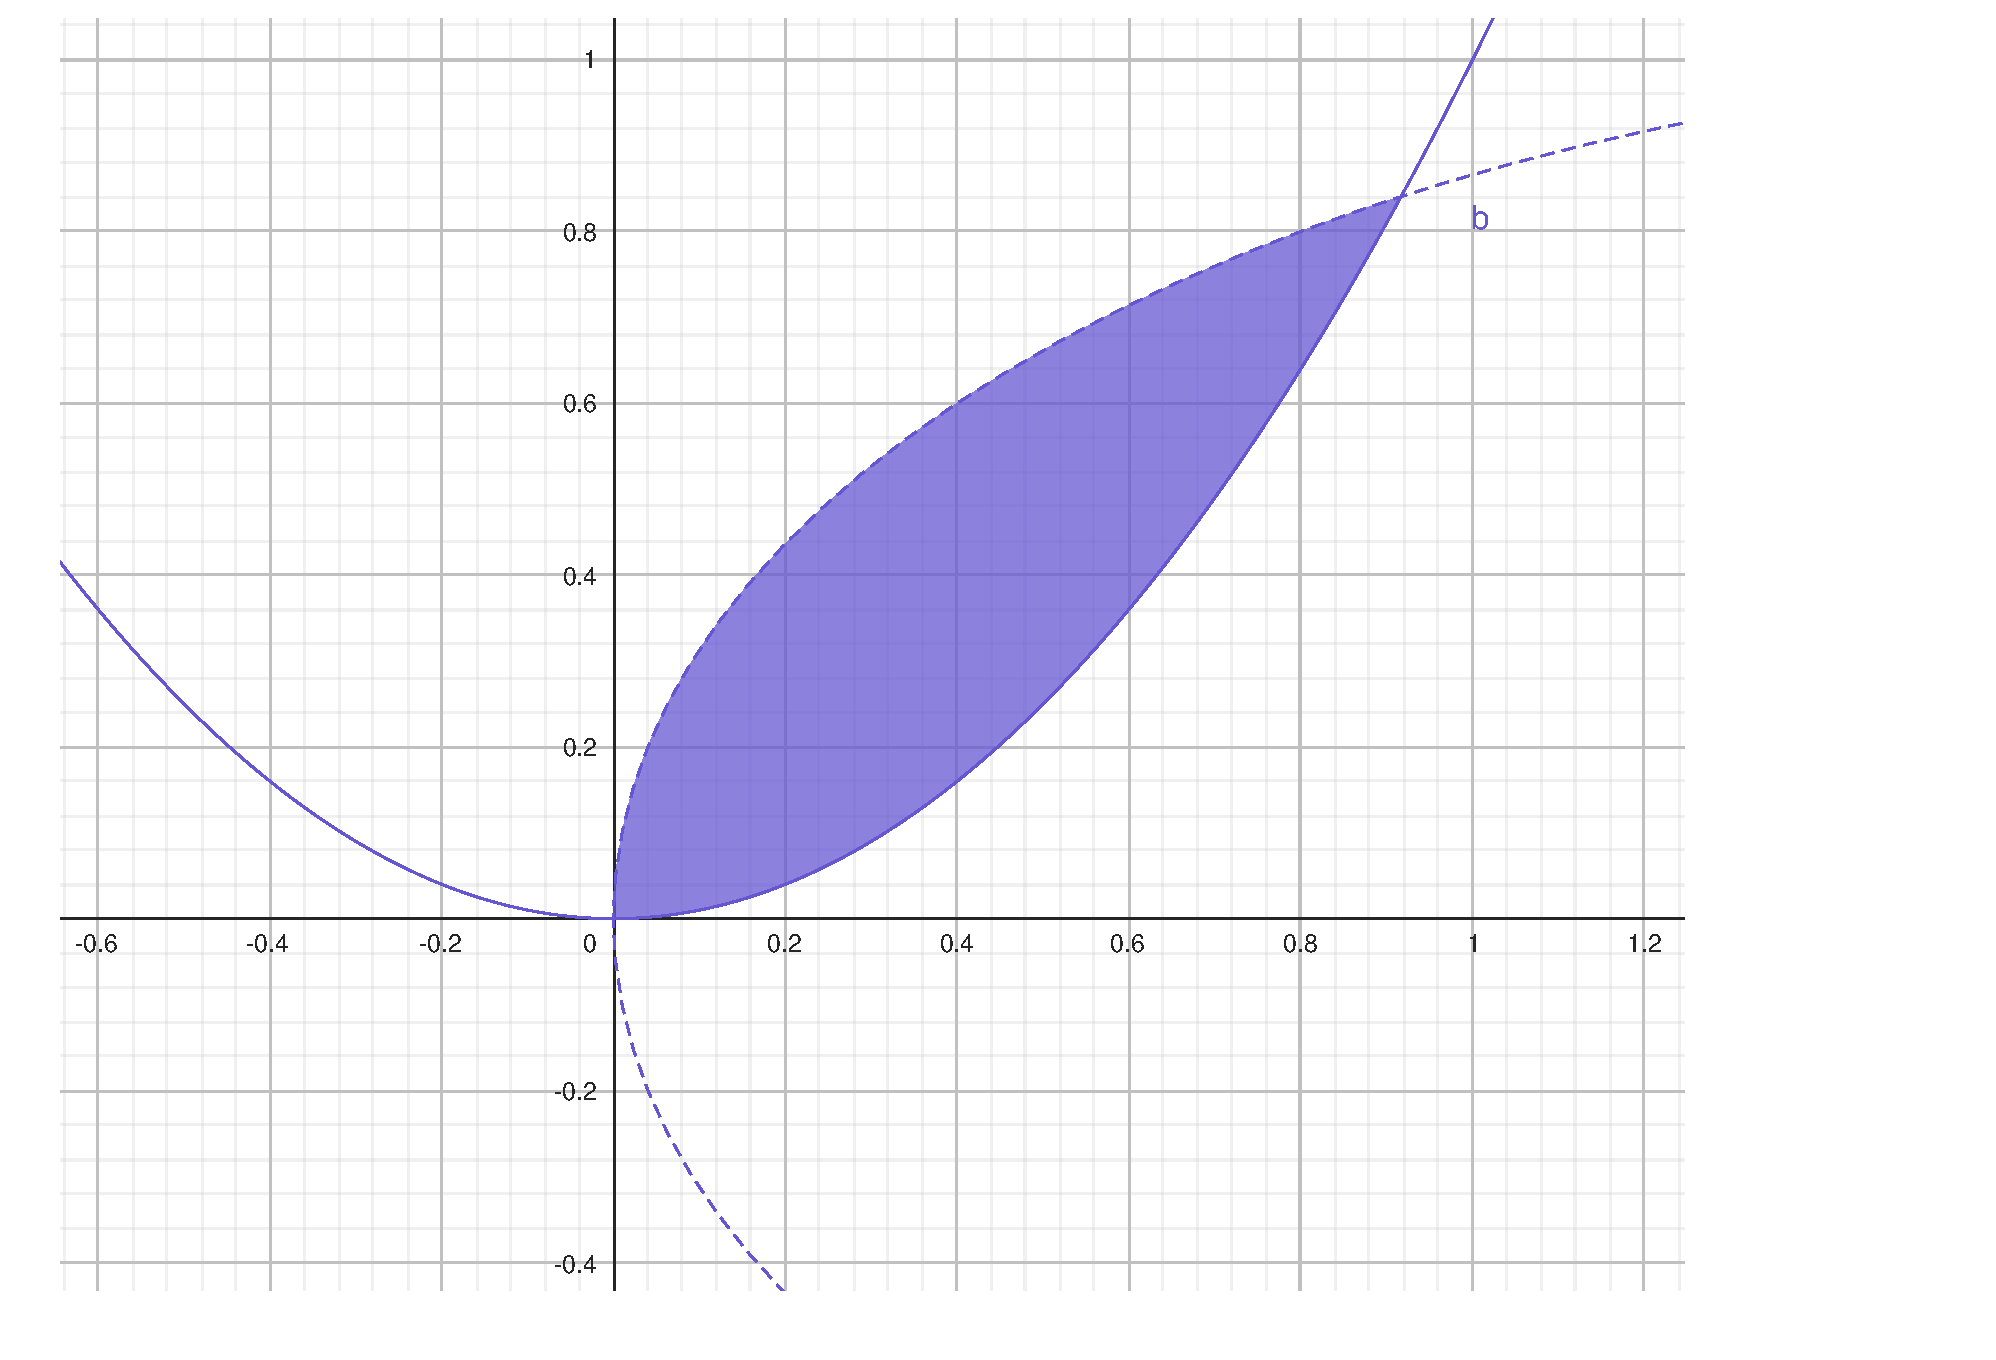
\includegraphics[width=\textwidth]{img/grafico-ex3-3.pdf}
		\caption*{Grafico del dominio completo.}
	\end{figure}\newpage

	\subsubsection{Dimostrazione che un punto sia interno al dominio}

	Una richiesta banale ma che potrebbe capitare, nonostante sia molto raro, è la seguente (estratta dall'esame del 25/06/2021): \textcolor{Green4}{\textbf{\emph{Sia $D\subset\mathbb{R}^{2}$ il dominio naturale della funzione:}}
	\begin{equation*}
		f\left(x,y\right) = \sqrt{y-x^{2}}-\ln\left(4x-x^{2}-4y^{2}\right)
	\end{equation*}
	\textbf{\emph{Si dimostri che il punto $P\left(\frac{1}{2}, \frac{1}{2}\right)$ è interno all'insieme $D$.}}}\newline

	\noindent
	Il \textbf{primo passo} è prendere le disuguaglianze del dominio e considerarle in modo stretto, ovvero:
	\begin{equation*}
		\begin{array}{lcl}
			y-x^{2} \ge 0			& \longrightarrow & y-x^{2} > 0 \\
			4x - x^{2} - 4y^{2} > 0	& \longrightarrow & 4x - x^{2} - 4y^{2} > 0
		\end{array}
	\end{equation*}
	Il \textbf{secondo passo} è sostituire i valori del punto dato dall'esercizio e verificare la veridicità delle disuguaglianze. In questo caso, si sostituisce il punto $P\left(\frac{1}{2}, \frac{1}{2}\right)$ all'interno delle due disuguaglianze:
	\begin{equation*}
		\begin{array}{lcl}
			y -x^{2} > 0			& \longrightarrow & \dfrac{1}{2} - \dfrac{1^{2}}{2^{2}} > 0 \Longrightarrow \dfrac{1}{4} > 0 \hspace{1em} \textcolor{Green4}{\checkmark} \\ [1em]
			4x - x^{2} - 4y^{2} > 0	& \longrightarrow & 4 \cdot \dfrac{1}{2} - \dfrac{1^{2}}{2^{2}} - 4 \cdot \dfrac{1^{2}}{2^{2}} > 0 \Longrightarrow \dfrac{3}{4} > 0 \hspace{1em} \textcolor{Green4}{\checkmark}
		\end{array}
	\end{equation*}
	Il punto $P$ rispetta entrambe le disuguaglianze, quindi è un punto interno al dominio.\newpage

	\subsubsection{Direzione della funzione affinché essa sia di massima crescita}\label{par: direzione della funzione affinché essa sia di massima crescita}

	Una richiesta che si può trovare negli esami ma non è tra le più richieste, è la seguente: \textcolor{Green4}{\textbf{\emph{Sia $D\subset\mathbb{R}^{2}$ il dominio naturale della funzione:}}
	\begin{equation*}
		f\left(x,y\right) = \sqrt{y-x^{2}}-\ln\left(4x-x^{2}-4y^{2}\right)
	\end{equation*}
	\textbf{\emph{In quale direzione ci si deve muovere da $P$ per garantire a $f$ la massima crescita?}}}\newline

	\noindent
	La direzione $\overrightarrow{v}$ di massima crescita è quella del gradiente di $f$ nel punto $P$. Per cui, per calcolare il gradiente sono necessari due passaggi fondamentali. Il \textbf{primo passo} è calcolare la derivata parziale rispetto a $x$:
	\begin{equation*}
		\begin{array}{rcl}
			f\left(x,y\right) &=& \sqrt{y-x^{2}}-\ln\left(4x-x^{2}-4y^{2}\right) \\ [1em]
			f\left(x,y\right) &=& \dfrac{\partial}{\partial x}\left( \sqrt{y-x^{2}}-\ln\left(4x-x^{2}-4y^{2}\right) \right) \\ [1.5em]
			&\downarrow& \text{si utilizza la regola } \frac{\partial}{\partial x}\left(f+g\right) = \frac{\partial}{\partial x}\left(f\right) + \frac{\partial}{\partial x}\left(g\right) \\ [1em]
			f\left(x,y\right) &=& \dfrac{\partial}{\partial x}\left( \sqrt{y-x^{2}}\right)- \dfrac{\partial}{\partial x}\left(\ln\left(4x-x^{2}-4y^{2}\right) \right) \\ [1.5em]
			&\downarrow& \text{derivata della radice quadrata per la derivata dell'argomento} \\ [1em]
			f\left(x,y\right) &=& \dfrac{1}{2\sqrt{y-x^{2}}}\cdot\left(-2x\right) - \dfrac{\partial}{\partial x}\left(\ln\left(4x-x^{2}-4y^{2}\right) \right) \\ [1.5em]
			&\downarrow& \text{derivata del logaritmo per la derivata dell'argomento} \\ [1em]
			f\left(x,y\right) &=& \dfrac{1}{2\sqrt{y-x^{2}}}\cdot\left(-2x\right) - \dfrac{1}{4x-x^{2}-4y^{2}} \cdot \left(4-2x\right) \\ [1.5em]
			&\downarrow& \text{semplificazioni} \\ [1em]
			\dfrac{\partial f}{\partial x}\left(x,y\right) &=& -\dfrac{x}{\sqrt{y-x^{2}}} - \dfrac{4-2x}{4x-x^{2}-4y^{2}} \\ [1.5em]
		\end{array}
	\end{equation*}\newpage

	\noindent
	Il \textbf{secondo passo} è calcolare la derivata parziale rispetto a $y$:
	\begin{equation*}
		\begin{array}{rcl}
			f\left(x,y\right) &=& \sqrt{y-x^{2}}-\ln\left(4x-x^{2}-4y^{2}\right) \\ [1em]
			f\left(x,y\right) &=& \dfrac{\partial}{\partial y}\left( \sqrt{y-x^{2}}-\ln\left(4x-x^{2}-4y^{2}\right) \right) \\ [1.5em]
			&\downarrow& \text{si utilizza la regola } \frac{\partial}{\partial y}\left(f+g\right) = \frac{\partial}{\partial y}\left(f\right) + \frac{\partial}{\partial y}\left(g\right) \\ [1em]
			f\left(x,y\right) &=& \dfrac{\partial}{\partial y}\left( \sqrt{y-x^{2}}\right) - \dfrac{\partial}{\partial y}\left(\ln\left(4x-x^{2}-4y^{2}\right) \right) \\ [1.5em]
			&\downarrow& \text{derivata della radice quadrata per la derivata dell'argomento} \\ [1em]
			f\left(x,y\right) &=& \dfrac{1}{2\sqrt{y-x^{2}}}\cdot\left(1\right) - \dfrac{\partial}{\partial y}\left(\ln\left(4x-x^{2}-4y^{2}\right) \right) \\ [1.5em]
			&\downarrow& \text{derivata del logaritmo per la derivata dell'argomento} \\ [1em]
			\dfrac{\partial f}{\partial y} \left(x,y\right) &=& \dfrac{1}{2\sqrt{y-x^{2}}} - \dfrac{1}{4x-x^{2}-4y^{2}}\cdot\left(-8y\right) \\ [1.5em]
			\dfrac{\partial f}{\partial y} \left(x,y\right) &=& \dfrac{1}{2\sqrt{y-x^{2}}} + \dfrac{8y}{4x-x^{2}-4y^{2}}
		\end{array}
	\end{equation*}\newpage

	\noindent
	Il \textbf{terzo passo} è quello di andare a sostituire i valori del punto $P$ all'interno delle derivate parziali. Così facendo, si troverà la direzione di massima crescita, ovvero il gradiente:
	\begin{equation*}
		\begin{array}{rcl}
			\dfrac{\partial f}{\partial x}\left(x,y\right) &=& -\dfrac{x}{\sqrt{y-x^{2}}} - \dfrac{4-2x}{4x-x^{2}-4y^{2}} \\ [1.5em]
			\dfrac{\partial f}{\partial x}\left(\dfrac{1}{2},\dfrac{1}{2}\right) &=& -\dfrac{\dfrac{1}{2}}{\sqrt{\dfrac{1}{2}-\dfrac{1^{2}}{2^{2}}}} - \dfrac{4-2 \cdot \dfrac{1}{2}}{4 \cdot \dfrac{1}{2} - \dfrac{1^{2}}{2^{2}} -4 \cdot \dfrac{1^{2}}{2^{2}}} \\ [3em]
			\dfrac{\partial f}{\partial x}\left(\dfrac{1}{2},\dfrac{1}{2}\right) &=& -1 - \dfrac{3}{2 - \dfrac{1}{4} - 1} \\ [1.5em]
			\dfrac{\partial f}{\partial x}\left(\dfrac{1}{2},\dfrac{1}{2}\right) &=& -5 \\ [3em]
			\dfrac{\partial f}{\partial y}\left(x,y\right) &=& \dfrac{1}{2\sqrt{y-x^{2}}} + \dfrac{8y}{4x-x^{2}-4y^{2}} \\ [1.5em]
			\dfrac{\partial f}{\partial y}\left(\dfrac{1}{2},\dfrac{1}{2}\right) &=& \dfrac{1}{2\sqrt{\dfrac{1}{2} - \dfrac{1^{2}}{2^{2}}}} + \dfrac{8 \cdot \dfrac{1}{2}}{4 \cdot \dfrac{1}{2} - \dfrac{1^{2}}{2^{2}} - 4 \cdot \dfrac{1^{2}}{2^{2}}} \\ [3em]
			\dfrac{\partial f}{\partial y}\left(\dfrac{1}{2},\dfrac{1}{2}\right) &=& 1 + \dfrac{4}{2 - \dfrac{1}{4} - 1} \\ [1.5em]
			\dfrac{\partial f}{\partial y}\left(\dfrac{1}{2},\dfrac{1}{2}\right) &=& \dfrac{19}{3}
		\end{array}
	\end{equation*}
	Si conclude l'esercizio:
	\begin{equation*}
		\overrightarrow{v} = \nabla f\left(P\right) = \left(-5, \dfrac{19}{3}\right)
	\end{equation*}\newpage

	\subsubsection{Specificare se un dominio è aperto/chiuso, limitato/illimitato, connesso/sconnesso, compatto}

	Questa richiesta è molto probabile che ci sia all'esame. Solitamente, viene accoppiata con la scrittura del dominio e della sua rappresentazione (pagina \pageref{par: rappresentare la funzione nel piano cartesiano}). Un esempio di tema d'esame (03/03/2023): \textcolor{Green4}{\textbf{\emph{Data la funzione:}}
	\begin{equation*}
		f\left(x,y\right) = y e^{\sqrt{x-2y}} - \ln\left(xy\right)
	\end{equation*}
	\textbf{\emph{Determinare analiticamente il suo dominio naturale $D$ e poi rappresentarlo nel piano cartesiano. Stabilire se $D$ è un insieme limitato/illimitato, aperto/chiuso, connesso/sconnesso (motivare le risposte!).}}}\newline

	\noindent
	Prima di tutto si stabilisce il dominio:
	\begin{equation*}
		D = \left\{\left(x,y\right) \in \mathbb{R}^{2} \: : \: \left(x-2y \ge 0\right) \land \left(xy > 0\right)\right\}
	\end{equation*}
	Ovvero si impone le condizioni di esistenza sulla radice quadrata e il logaritmo. La sua rappresentazione grafica:
	\begin{figure}[!htp]
		\centering
		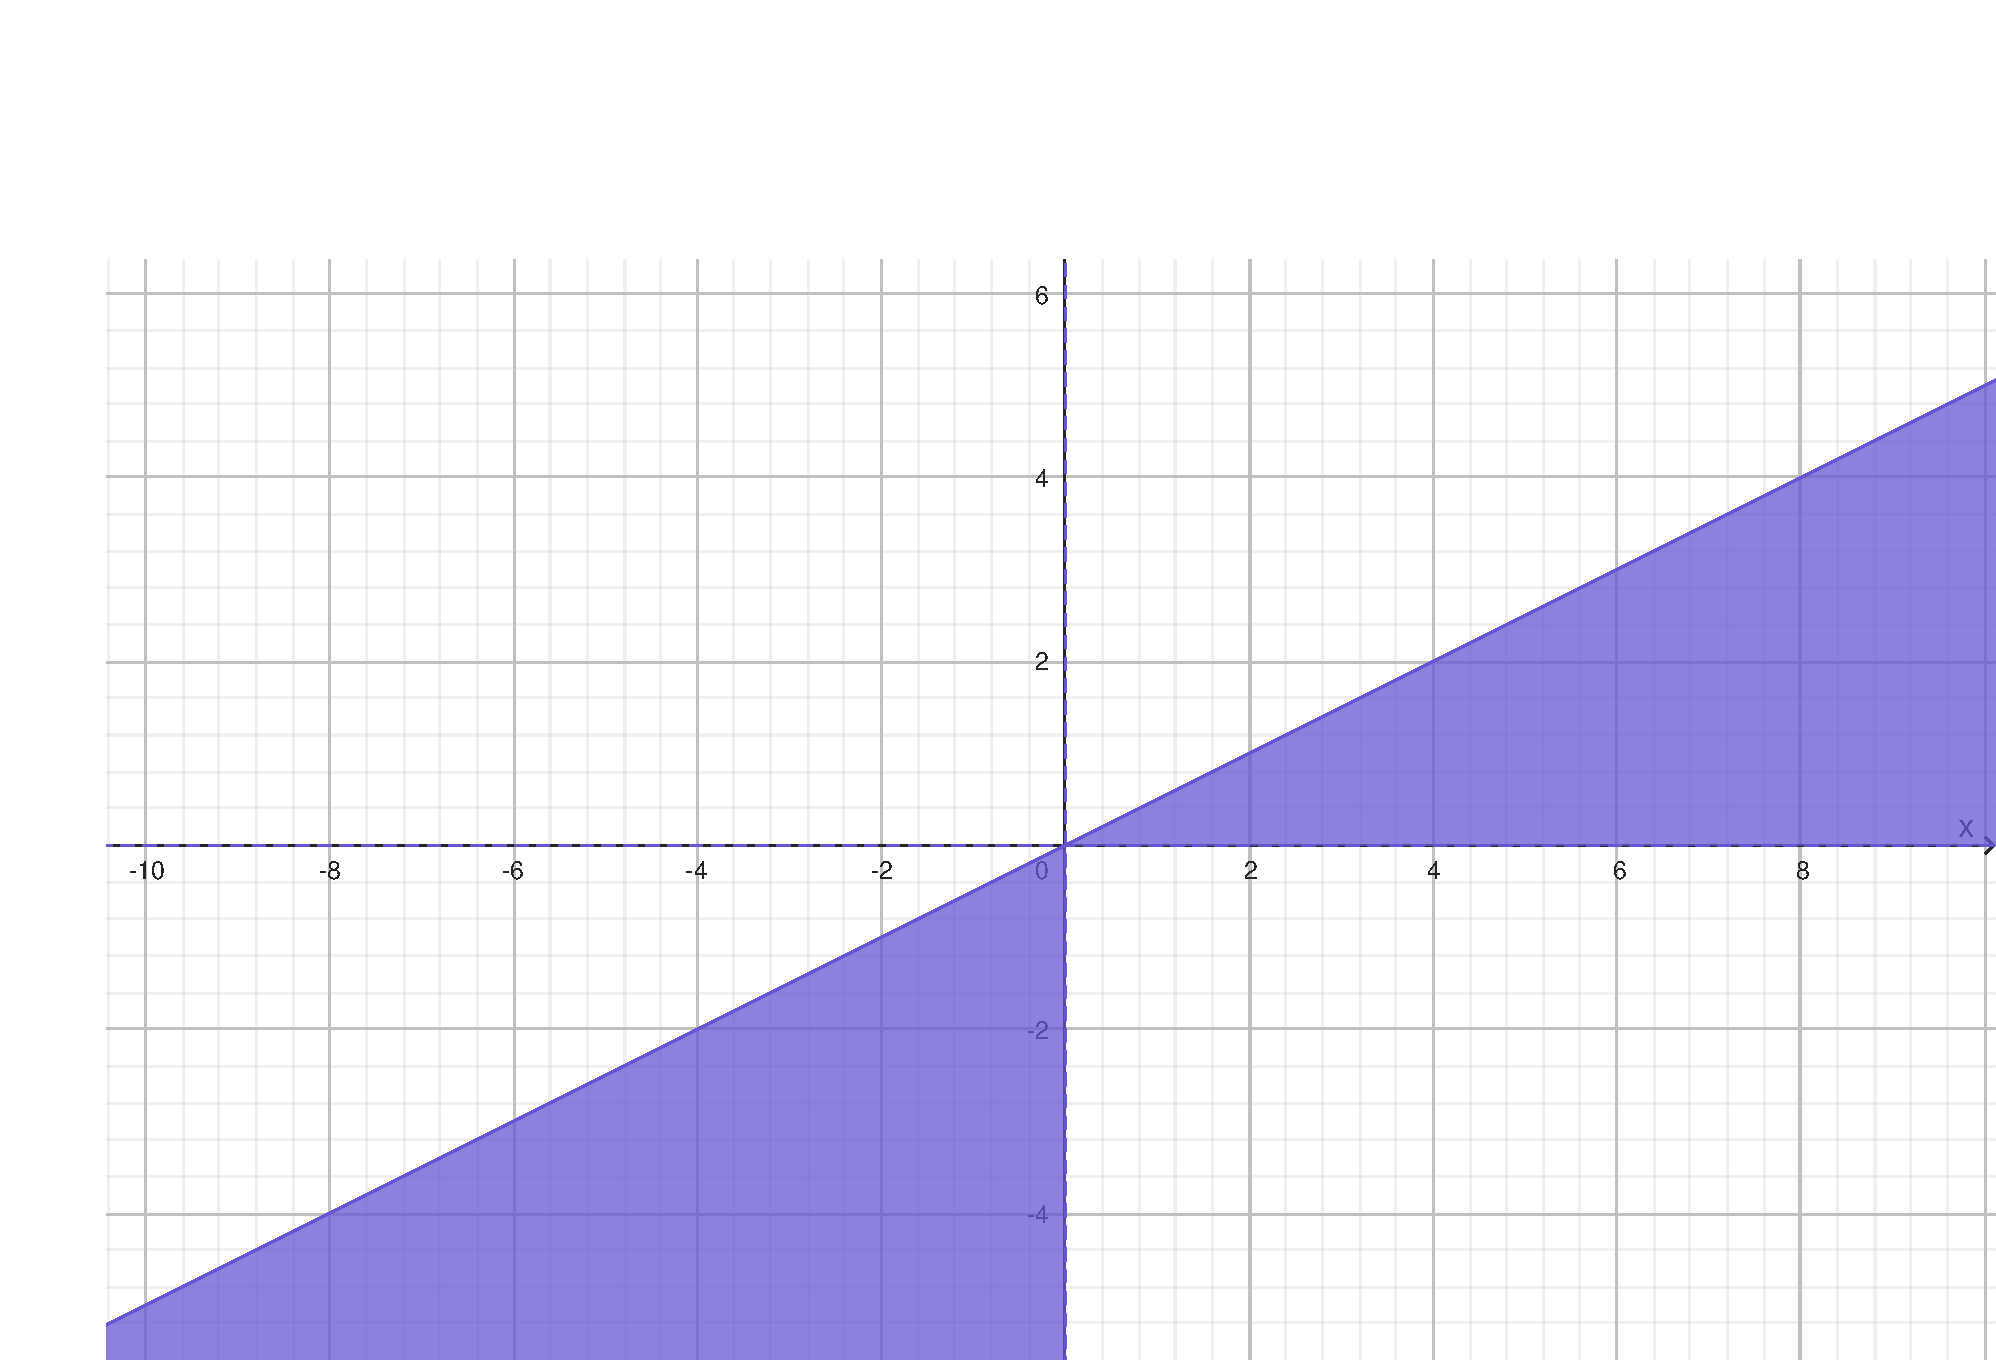
\includegraphics[width=\textwidth]{img/grafico-ex3-4.pdf}
	\end{figure}
	\begin{itemize}
		\item \textbf{Limitato o illimitato?} Il dominio è illimitato, dato che continua all'infinito, ovvero non esiste una palla con centro l'origine e raggio $r \in \mathbb{R}$ che contiene $D$.
		
		\item \textbf{Aperto o chiuso?} Il dominio non è né chiuso né aperto poiché contiene alcuni punti della sua frontiera ma non tutti.
		
		\item \textbf{Connesso o sconnesso?} Il dominio è sconnesso poiché non è connesso per archi. Infatti, come si può vedere dal grafico del dominio, quest'ultimo è l'unione di due insiemi.
	\end{itemize}
	Nell'esame del 07/02/2023, la funzione di riferimento e il dominio erano:
	\begin{equation*}
		\begin{array}{rcl}
			f\left(x,y\right) &=& y + \dfrac{1}{\sqrt{1 - \ln\left(y-x^{2}\right)}} - \ln\left(x\right) \\ [1.5em]
			D &=& \left\{\left(x,y\right) \in \mathbb{R}^{2} \: : \: \left(y > x^{2}\right) \land \left(y < x^{2} + e\right) \land \left(x > 0\right)\right\}
		\end{array}
	\end{equation*}
	\begin{figure}[!htp]
		\centering
		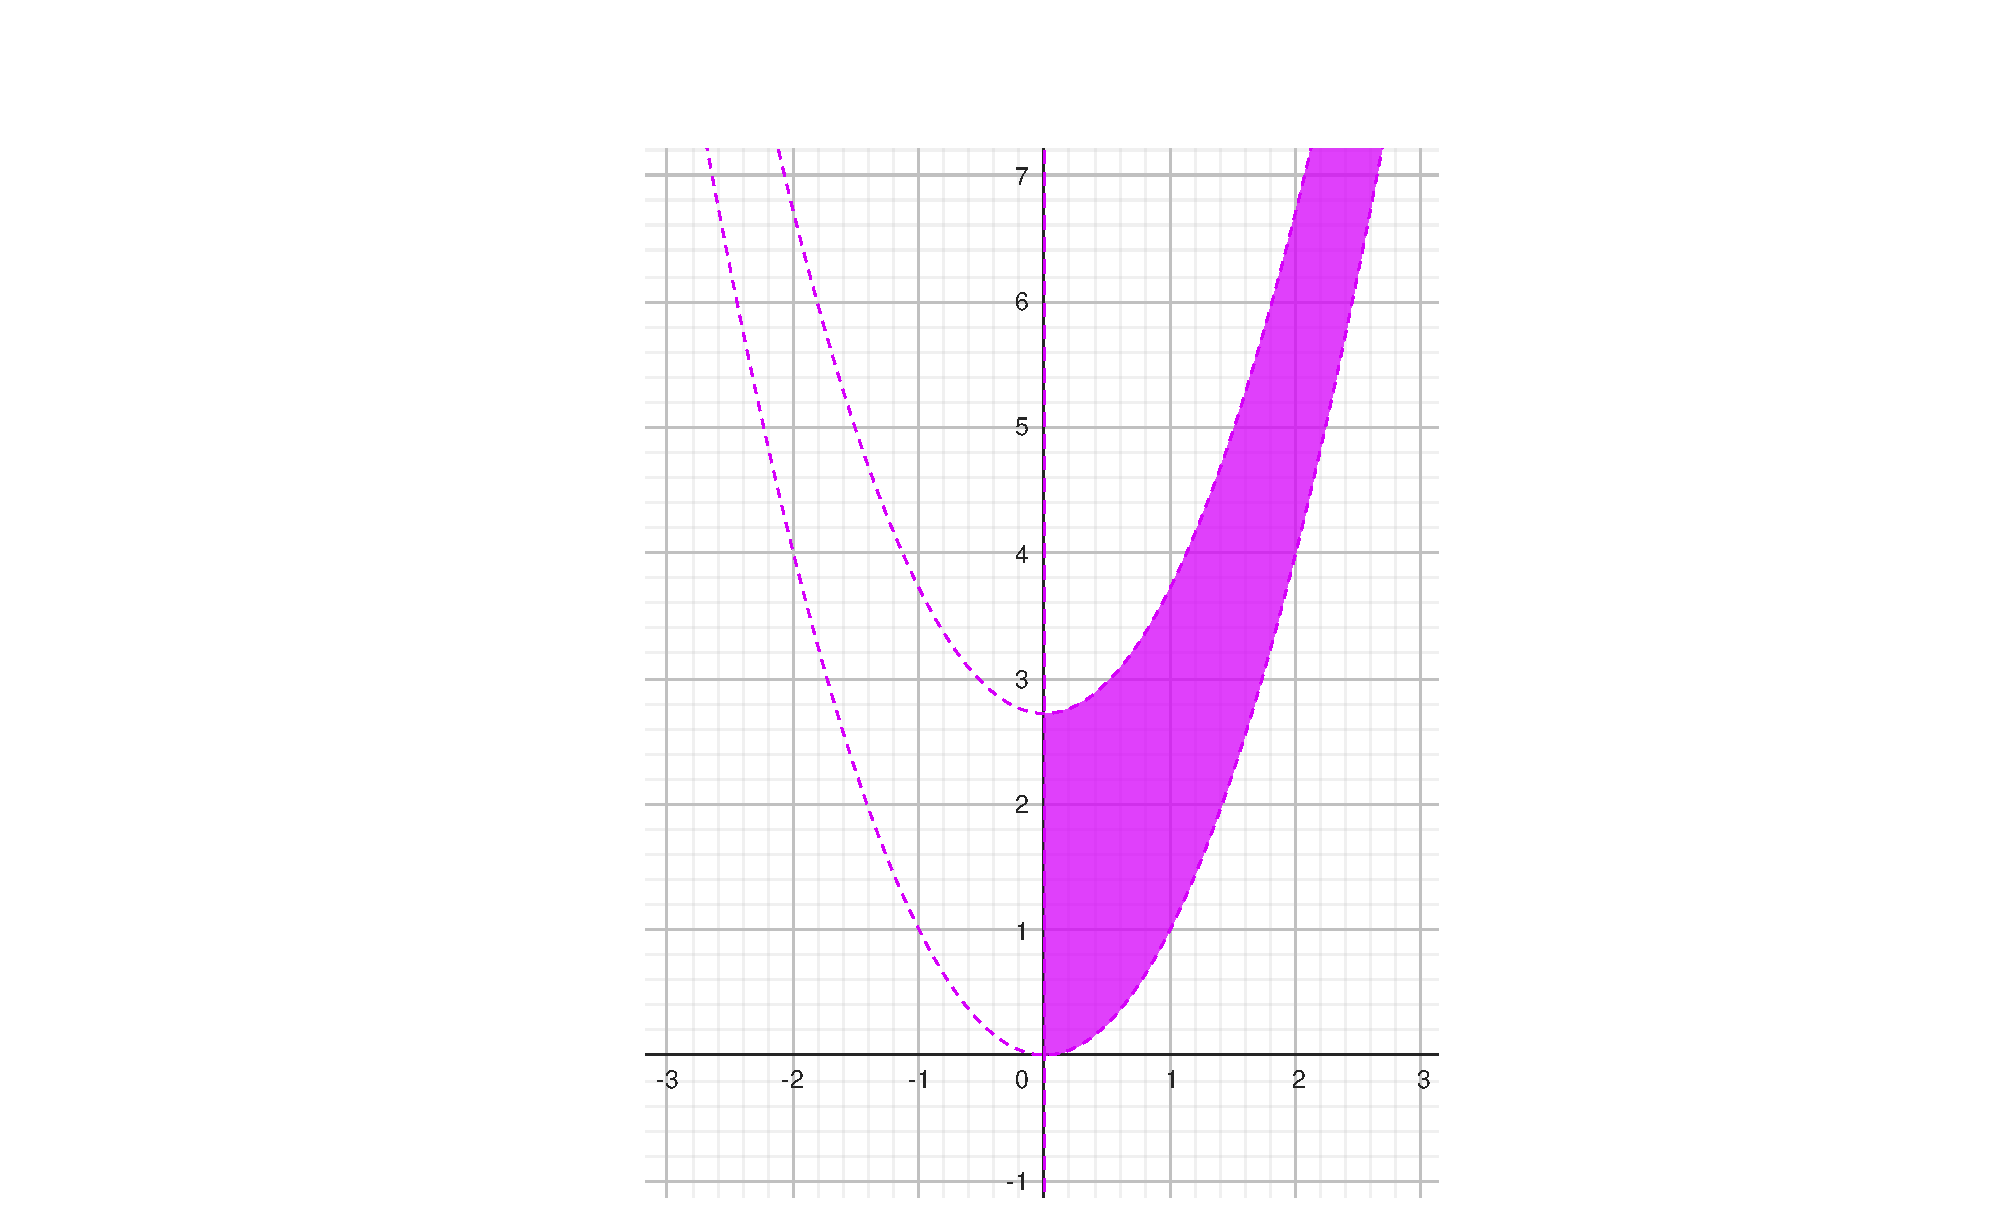
\includegraphics[width=.8\textwidth]{img/grafico-ex3-5.pdf}
		\caption*{Dominio della funzione.}
	\end{figure}

	\noindent
	In questo caso, il dominio è illimitato per lo stesso motivo dell'esercizio precedente; il dominio è aperto poiché tutti i punti sono interni e inoltre è connesso per archi.\newpage

	\subsubsection{Trovare l'equazione al piano tangente}\label{par: trovare l'equazione al piano tangente}

	Uno degli esercizi più richiesti insieme alla derivata direzionale, è quello di trovare l'equazione al piano tangente. Si prenda in considerazione il tema d'esame del 07/02/2023 in cui veniva chiesto: \textcolor{Green4}{\textbf{\emph{Data la funzione:}}
	\begin{equation*}
		f\left(x,y\right) = y + \dfrac{1}{\sqrt{1 - \ln\left(y - x^{2}\right)}} - \ln\left(x\right)
	\end{equation*}
	\textbf{\emph{Scrivere l'equazione del piano tangente al grafico di $f$ nel punto $\left(1, 2, f\left(1,2\right)\right)$.}}}\newline

	\noindent
	Anche in questo caso, come accadeva nel caso in cui si doveva trovare la direzione della funzione affinché essa sia di massima crescita (pagina \pageref{par: direzione della funzione affinché essa sia di massima crescita}), è necessario calcolare le derivate parziali di $f\left(x,y\right)$. Quindi, il \textbf{primo passo} è calcolare la derivata parziale rispetto a $x$:
	\begin{equation*}
		\begin{array}{rcl}
			f\left(x,y\right) &=& y + \dfrac{1}{\sqrt{1 - \ln\left(y - x^{2}\right)}} - \ln\left(x\right) \\ [1.5em]
			f\left(x,y\right) &=& \dfrac{\partial}{\partial x} \left( y + \dfrac{1}{\sqrt{1 - \ln\left(y - x^{2}\right)}} - \ln\left(x\right) \right) \\ [2em]
			&\downarrow& \text{si utilizza la regola } \frac{\partial}{\partial x}\left(f+g\right) = \frac{\partial}{\partial x}\left(f\right) + \frac{\partial}{\partial x}\left(g\right) \\ [1em]
			f\left(x,y\right) &=& \dfrac{\partial}{\partial x} \left(y\right) + \dfrac{\partial}{\partial x} \left(\dfrac{1}{\sqrt{1 - \ln\left(y - x^{2}\right)}}\right) - \dfrac{\partial}{\partial x}\left(\ln\left(x\right)\right) \\ [1.5em]
			&\downarrow& \text{si utilizza la regola } \frac{\partial}{\partial x}\left(\frac{1}{f}\right) = -\frac{\frac{\partial}{\partial x}\left(f\right)}{f^{2}} \\ [1em]
			\dfrac{\partial f}{\partial x}\left(x,y\right) &=& 0 - \dfrac{\dfrac{1}{2\sqrt{1-\ln\left(y-x^{2}\right)}} \cdot \left(-\dfrac{1}{y-x^{2}} \cdot \left(-2x\right)\right)}{\sqrt{1 - \ln\left(y - x^{2}\right)}^{2}} - \left(\dfrac{1}{x} \cdot \left(1\right)\right) \\ [2em]
			\dfrac{\partial f}{\partial x}\left(x,y\right) &=& -\dfrac{\dfrac{1}{2\sqrt{1-\ln\left(y-x^{2}\right)}} \cdot \left(\dfrac{2x}{y-x^{2}}\right)}{1 - \ln\left(y - x^{2}\right)} - \dfrac{1}{x} \\ [2em]
			\dfrac{\partial f}{\partial x}\left(x,y\right) &=& -\dfrac{\dfrac{x}{\sqrt{1-\ln\left(y-x^{2}\right)} \cdot \left(y-x^{2}\right)}}{1-\ln\left(y-x^{2}\right)} - \dfrac{1}{x} \\ [2em]
			\dfrac{\partial f}{\partial x}\left(x,y\right) &=& -\dfrac{x}{\sqrt{1 - \ln\left(y-x^{2}\right)} \cdot \left(y-x^{2}\right) \cdot \left(1 - \ln\left(y-x^{2}\right)\right)} - \dfrac{1}{x}
		\end{array}
	\end{equation*}\newpage

	\nointerlineskip
	Il \textbf{secondo passo} è calcolare la derivata parziale rispetto a $y$:
	\begin{equation*}
		\begin{array}{rcl}
			f\left(x,y\right) &=& y + \dfrac{1}{\sqrt{1 - \ln\left(y - x^{2}\right)}} - \ln\left(x\right) \\ [1.5em]
			f\left(x,y\right) &=& \dfrac{\partial}{\partial y} \left( y + \dfrac{1}{\sqrt{1 - \ln\left(y - x^{2}\right)}} - \ln\left(x\right) \right) \\ [2em]
			&\downarrow& \text{si utilizza la regola } \frac{\partial}{\partial y}\left(f+g\right) = \frac{\partial}{\partial y}\left(f\right) + \frac{\partial}{\partial y}\left(g\right) \\ [1em]
			f\left(x,y\right) &=& \dfrac{\partial}{\partial y} \left(y\right) + \dfrac{\partial}{\partial y} \left(\dfrac{1}{\sqrt{1 - \ln\left(y - x^{2}\right)}}\right) - \dfrac{\partial}{\partial y}\left(\ln\left(x\right)\right) \\ [1.5em]
			&\downarrow& \text{si utilizza la regola } \frac{\partial}{\partial y}\left(\frac{1}{f}\right) = -\frac{\frac{\partial}{\partial y}\left(f\right)}{f^{2}} \\ [1em]
			\dfrac{\partial f}{\partial y}\left(x,y\right) &=& 1 - \dfrac{\dfrac{1}{2\sqrt{1-\ln\left(y-x^{2}\right)}} \cdot \left(-\dfrac{1}{y-x^{2}} \cdot 1\right)}{\sqrt{1-\ln\left(y-x^{2}\right)}^{2}} - 0 \\ [2em]
			\dfrac{\partial f}{\partial y}\left(x,y\right) &=& 1 + \dfrac{1}{2\sqrt{1-\ln\left(y-x^{2}\right)} \cdot \left(y-x^{2}\right) \cdot \left(1-\ln\left(y-x^{2}\right)\right)}
		\end{array}
	\end{equation*}
	Il \textbf{terzo passo} è scrivere il gradiente valutato nel punto dato, ovvero in $P\left(1,2\right)$. Quindi, si prendono le derivate parziali trovate, si sostituiscono i valori e si utilizzano nel gradiente:
	\begin{equation*}
		\begin{array}{rcl}
			\dfrac{\partial f}{\partial x}\left(x,y\right) &=& -\dfrac{x}{\sqrt{1 - \ln\left(y-x^{2}\right)} \cdot \left(y-x^{2}\right) \cdot \left(1 - \ln\left(y-x^{2}\right)\right)} - \dfrac{1}{x} \\ [1.5em]
			\dfrac{\partial f}{\partial x}\left(1,2\right) &=& -\dfrac{1}{\sqrt{1 - \ln\left(2-1^{2}\right)} \cdot \left(2-1^{2}\right) \cdot \left(1 - \ln\left(2-1^{2}\right)\right)} - \dfrac{1}{1} \\ [1.5em]
			\dfrac{\partial f}{\partial x}\left(1,2\right) &=& -\dfrac{1}{\sqrt{1 - \ln\left(1\right)} \cdot 1 \cdot \left(1 - \ln\left(1\right)\right)} - 1 \\ [1.5em]
			\dfrac{\partial f}{\partial x}\left(1,2\right) &=& -\dfrac{1}{1 \cdot 1 \cdot 1} - 1 \\ [1.5em]
			\dfrac{\partial f}{\partial x}\left(1,2\right) &=& -2 \\ [2em]
			\dfrac{\partial f}{\partial y}\left(x,y\right) &=& 1 + \dfrac{1}{2\sqrt{1-\ln\left(y-x^{2}\right)} \cdot \left(y-x^{2}\right) \cdot \left(1-\ln\left(y-x^{2}\right)\right)} \\ [1.5em]
			\dfrac{\partial f}{\partial y}\left(1,2\right) &=& 1 + \dfrac{1}{2\sqrt{1-\ln\left(2-1^{2}\right)} \cdot \left(2-1^{2}\right) \cdot \left(1-\ln\left(2-1^{2}\right)\right)} \\ [1.5em]
			\dfrac{\partial f}{\partial y}\left(1,2\right) &=& 1 + \dfrac{1}{2 \cdot 1 \cdot 1 \cdot 1} \\ [1.5em]
			\dfrac{\partial f}{\partial y}\left(1,2\right) &=& \dfrac{3}{2}
		\end{array}
	\end{equation*}\newpage

	\noindent
	Per cui il gradiente corrisponde al valore:
	\begin{equation*}
		\nabla f\left(P\right) = \nabla f\left(1,2\right) = \left(-2, \dfrac{3}{2}\right)
	\end{equation*}
	Il \textbf{quarto e ultimo passo} è scrivere l'equazione del piano tangente. Il piano tangente nel punto $\left(x,y,\left(x_{0}, y_{0}\right)\right)$ è rappresentato dall'equazione:
	\begin{equation*}
		z = f\left(x_{0},y_{0}\right) + \dfrac{\partial f}{\partial x}\left(x_{0}, y_{0}\right)\left(x-x_{0}\right) + \dfrac{\partial f}{\partial y}\left(x_{0}, y_{0}\right)\left(y-y_{0}\right)
	\end{equation*}
	Dove $f\left(x,y\right)$ è la funzione e $\left(x_{0},y_{0}\right)$ è il punto in cui è differenziabile.

	Grazie a questo richiamo di teoria, adesso è possibile scrivere l'equazione del piano tangente. Quindi, si prende il punto differenziabile, cioè $P\left(1,2\right)$, e si sostituisce nell'equazione iniziale:
	\begin{equation*}
		\begin{array}{rcl}
			f\left(x,y\right) &=& y + \dfrac{1}{\sqrt{1 - \ln\left(y - x^{2}\right)}} - \ln\left(x\right) \\ [1.5em]
			f\left(1,2\right) &=& 2 + \dfrac{1}{\sqrt{1 - \ln\left(2 - 1^{2}\right)}} - \ln\left(1\right) \\ [1.5em]
			f\left(1,2\right) &=& 2 + \dfrac{1}{1} - 0 \\ [1.5em]
			f\left(1,2\right) &=& 3
		\end{array}
	\end{equation*}
	E infine si sostituiscono i valori calcolati nell'equazione del piano tangente:
	\begin{equation*}
		z = 3 - 2\left(x - 1\right) + \dfrac{3}{2}\left(y-2\right) = 3 - 2x +2 + \dfrac{3}{2}y - 3 = -2x + \dfrac{3}{2}y + 2
	\end{equation*}\newpage

	\subsubsection{Calcolare il gradiente della funzione ($\nabla f$)}\label{par: calcolare il gradiente della funzione}

	Esercizio difficile che venga richiesto, ma una volta è capitato, è la richiesta esplicita di calcolare il gradiente. Solitamente viene richiesto di trovare la massima crescita della funzione, cioè il gradiente, o la derivata direzionale. In questo caso, si calcola direttamente il gradiente come è stato fatto nei precedenti capitoli. Si riporta comunque i passaggi da eseguire. Si faccia riferimento al testo d'esame del 15/09/2021, gruppo A: \textcolor{Green4}{\textbf{\emph{Data la funzione:}}
	\begin{equation*}
		f\left(x,y\right) = \log\left(x^{2} - 4x + 4y^{2}\right) - \sqrt{2x - x^{2}}
	\end{equation*}
	\textbf{\emph{Calcolare $\nabla f\left(P\right)$, dove $P$ è il punto di coordinate $(1,2)$.}}}\newline
	
	\noindent
	Il \textbf{primo passo} è calcolare la derivata parziale rispetto $x$:
	\begin{equation*}
		\begin{array}{rcl}
			f\left(x,y\right) &=& \log\left(x^{2} - 4x + 4y^{2}\right) - \sqrt{2x - x^{2}} \\ [.5em]
			f\left(x,y\right) &=& \dfrac{\partial}{\partial x} \left(\log\left(x^{2} - 4x + 4y^{2}\right) - \sqrt{2x - x^{2}}\right) \\ [1.5em]
			f\left(x,y\right) &=& \dfrac{\partial}{\partial x}\left(\log\left(x^{2}-4x+4y^{2}\right)\right) - \dfrac{\partial}{\partial x}\left(\sqrt{2x-x^{2}}\right) \\ [1.5em]
			\dfrac{\partial f}{\partial x}\left(x,y\right) &=& \dfrac{1}{x^{2}-4x+4y^{2}} \cdot \left(2x - 4\right) - \dfrac{1}{2\sqrt{2x-x^{2}}} \cdot \left(2-2x\right) \\ [1.5em]
			\dfrac{\partial f}{\partial x}\left(x,y\right) &=& \dfrac{2x - 4}{x^{2}-4x+4y^{2}} - \dfrac{2-2x}{2\sqrt{2x-x^{2}}}
		\end{array}
	\end{equation*}
	Il \textbf{secondo passo} è calcolare la derivata parziale rispetto $y$:
	\begin{equation*}
		\begin{array}{rcl}
			f\left(x,y\right) &=& \log\left(x^{2} - 4x + 4y^{2}\right) - \sqrt{2x - x^{2}} \\ [.5em]
			f\left(x,y\right) &=& \dfrac{\partial}{\partial y} \left(\log\left(x^{2} - 4x + 4y^{2}\right) - \sqrt{2x - x^{2}}\right) \\ [1.5em]
			f\left(x,y\right) &=& \dfrac{\partial}{\partial y}\left(\log\left(x^{2}-4x+4y^{2}\right)\right) - \dfrac{\partial}{\partial y}\left(\sqrt{2x-x^{2}}\right) \\ [1.5em]
			\dfrac{\partial f}{\partial y}\left(x,y\right) &=& \dfrac{1}{x^{2}-4x+4y^{2}} \cdot \left(8y\right) - \dfrac{1}{2\sqrt{2x-x^{2}}} \cdot \left(0\right) \\ [1.5em]
			\dfrac{\partial f}{\partial y}\left(x,y\right) &=& \dfrac{8y}{x^{2} - 4x + 4y^{2}}
		\end{array}
	\end{equation*}
	Il \textbf{terzo passo} è sostituire il punto di coordinate $P\left(1,2\right)$ all'interno delle derivate parziali e calcolare il gradiente:
	\begin{equation*}
		\begin{array}{rcl}
			\dfrac{\partial f}{\partial x}\left(x,y\right) &=& \dfrac{2x - 4}{x^{2}-4x+4y^{2}} - \dfrac{2-2x}{2\sqrt{2x-x^{2}}} \\ [1.5em]
			\dfrac{\partial f}{\partial x}\left(1,2\right) &=& \dfrac{2 \cdot 1 - 4}{1^{2}-4 \cdot 1+4 \cdot 2^{2}} - \dfrac{2-2 \cdot 1}{2\sqrt{2 \cdot 1- 1^{2}}} \\ [1.5em]
			\dfrac{\partial f}{\partial x}\left(1,2\right) &=& -\dfrac{2}{13} - \dfrac{0}{2} = -\dfrac{2}{13}
		\end{array}
	\end{equation*}\newpage
	\begin{equation*}
		\begin{array}{rcl}
			\dfrac{\partial f}{\partial y}\left(x,y\right) &=& \dfrac{8y}{x^{2} - 4x + 4y^{2}} \\ [1.5em]
			\dfrac{\partial f}{\partial y}\left(1,2\right) &=& \dfrac{8 \cdot 2}{1^{2} - 4 \cdot 1 + 4 \cdot 2^{2}} \\ [1.5em]
			\dfrac{\partial f}{\partial y}\left(1,2\right) &=& \dfrac{16}{13}
		\end{array}
	\end{equation*}
	Il gradiente dunque corrisponde a:
	\begin{equation*}
		\nabla f\left(P\right) = \nabla f\left(1,2\right) = \left(-\dfrac{2}{13}, \dfrac{16}{13}\right)
	\end{equation*}\newpage

	\subsubsection{Calcolare la derivata direzionale}

	Un esercizio richiestissimo, è il calcolo della derivata direzionale. Un esercizio tipo è il seguente, estratto dall'esame del 15/09/2021, gruppo A: \textcolor{Green4}{\textbf{\emph{Data la funzione:}}
	\begin{equation*}
		f\left(x,y\right) = \log\left(x^{2} -4x + 4y^{2}\right) - \sqrt{2x - x^{2}}
	\end{equation*}
	\textbf{\emph{Calcolare la derivata direzionale di $f$ in $P$ rispetto al versore $\overrightarrow{v} = \left(\frac{\sqrt{3}}{2}, \frac{1}{2}\right)$.}}}\newline

	\noindent
	La derivata direzionale di una funzione in un punto rispetto ad un versore, non è altro che la moltiplicazione del gradiente della funzione in quel punto per il versore, ovvero:
	\begin{equation*}
		\nabla f\left(P\right) \cdot \overrightarrow{v}
	\end{equation*}
	Viene da sé che è necessario prima calcolare il gradiente e poi calcolare il versore. Come \textbf{primo passo} si calcolano le derivate parziali:
	\begin{equation*}
		\begin{array}{rcl}
			f\left(x,y\right) &=& \log\left(x^{2} - 4x + 4y^{2}\right) - \sqrt{2x - x^{2}} \\ [.5em]
			f\left(x,y\right) &=& \dfrac{\partial}{\partial x} \left(\log\left(x^{2} - 4x + 4y^{2}\right) - \sqrt{2x - x^{2}}\right) \\ [1.5em]
			f\left(x,y\right) &=& \dfrac{\partial}{\partial x}\left(\log\left(x^{2}-4x+4y^{2}\right)\right) - \dfrac{\partial}{\partial x}\left(\sqrt{2x-x^{2}}\right) \\ [1.5em]
			\dfrac{\partial f}{\partial x}\left(x,y\right) &=& \dfrac{1}{x^{2}-4x+4y^{2}} \cdot \left(2x - 4\right) - \dfrac{1}{2\sqrt{2x-x^{2}}} \cdot \left(2-2x\right) \\ [1.5em]
			\dfrac{\partial f}{\partial x}\left(x,y\right) &=& \dfrac{2x - 4}{x^{2}-4x+4y^{2}} - \dfrac{2-2x}{2\sqrt{2x-x^{2}}} \\ [3em]
			%
			f\left(x,y\right) &=& \log\left(x^{2} - 4x + 4y^{2}\right) - \sqrt{2x - x^{2}} \\ [.5em]
			f\left(x,y\right) &=& \dfrac{\partial}{\partial y} \left(\log\left(x^{2} - 4x + 4y^{2}\right) - \sqrt{2x - x^{2}}\right) \\ [1.5em]
			f\left(x,y\right) &=& \dfrac{\partial}{\partial y}\left(\log\left(x^{2}-4x+4y^{2}\right)\right) - \dfrac{\partial}{\partial y}\left(\sqrt{2x-x^{2}}\right) \\ [1.5em]
			\dfrac{\partial f}{\partial y}\left(x,y\right) &=& \dfrac{1}{x^{2}-4x+4y^{2}} \cdot \left(8y\right) - \dfrac{1}{2\sqrt{2x-x^{2}}} \cdot \left(0\right) \\ [1.5em]
			\dfrac{\partial f}{\partial y}\left(x,y\right) &=& \dfrac{8y}{x^{2} - 4x + 4y^{2}}
		\end{array}
	\end{equation*}
	(calcoli già eseguiti nel paragrafo precedente, li riportiamo per convenienza)\newpage
	
	\noindent
	Il \textbf{secondo passo} è sostituire il punto fornito $P\left(1,2\right)$ all'interno delle derivate parziali così da ottenere il gradiente:
	\begin{equation*}
		\begin{array}{rcl}
			\dfrac{\partial f}{\partial x}\left(x,y\right) &=& \dfrac{2x - 4}{x^{2}-4x+4y^{2}} - \dfrac{2-2x}{2\sqrt{2x-x^{2}}} \\ [1.5em]
			\dfrac{\partial f}{\partial x}\left(1,2\right) &=& \dfrac{2 \cdot 1 - 4}{1^{2}-4 \cdot 1+4 \cdot 2^{2}} - \dfrac{2-2 \cdot 1}{2\sqrt{2 \cdot 1- 1^{2}}} \\ [1.5em]
			\dfrac{\partial f}{\partial x}\left(1,2\right) &=& -\dfrac{2}{13} - \dfrac{0}{2} = -\dfrac{2}{13} \\ [2.5em]
			%
			\dfrac{\partial f}{\partial y}\left(x,y\right) &=& \dfrac{8y}{x^{2} - 4x + 4y^{2}} \\ [1.5em]
			\dfrac{\partial f}{\partial y}\left(1,2\right) &=& \dfrac{8 \cdot 2}{1^{2} - 4 \cdot 1 + 4 \cdot 2^{2}} \\ [1.5em]
			\dfrac{\partial f}{\partial y}\left(1,2\right) &=& \dfrac{16}{13}
		\end{array}
	\end{equation*}
	Il gradiente dunque corrisponde a:
	\begin{equation*}
		\nabla f\left(P\right) = \nabla f\left(1,2\right) = \left(-\dfrac{2}{13}, \dfrac{16}{13}\right)
	\end{equation*}
	Fin qua l'esercizio è identico al calcolo del gradiente della funzione (pagina \pageref{par: calcolare il gradiente della funzione}). Il \textbf{terzo passo} è eseguire la moltiplicazione tra il versore fornito dall'esercizio $\overrightarrow{v}$ e il gradiente calcolato:
	\begin{equation*}
		\nabla f\left(P\right) \cdot \overrightarrow{v} = \left(-\dfrac{2}{13} \cdot \dfrac{\sqrt{3}}{2}, \: \dfrac{16}{13} \cdot \dfrac{1}{2}\right) = \left(-\dfrac{\sqrt{3}}{13}, \: \dfrac{8}{13}\right) = -\dfrac{\sqrt{3}}{13} + \dfrac{8}{13} = \dfrac{-\sqrt{3} + 8}{13}
	\end{equation*}\newpage

	\subsection{Vari esercizi d'esame}

	\subsubsection{Esame del 10/07/2023 - Gruppo A}

	\textcolor{Green4}{\textbf{\emph{Data la funzione}}}
	\begin{equation*}
		f\left(x,y\right) = \sqrt[4]{2 - \left(x-1\right)^{2} - \left(y-1\right)^{2}} + e^{\frac{1}{x}}
	\end{equation*}
	\begin{enumerate}[label=\alph*)]
		\item \textcolor{Green4}{\textbf{\emph{(2 punti) determinare analiticamente il suo dominio naturale D e poi rappresentarlo (con cura!) nel piano cartesiano. Stabilire se D è un insieme limitato/illimitato, aperto/chiuso, connesso/sconnesso (motivare le risposte!)}}}
		
		\item \textcolor{Green4}{\textbf{\emph{(2 punti) calcolare $\dfrac{\partial f}{\partial \overrightarrow{v}}\left(1,2\right)$, con $\overrightarrow{v} = \left(-\dfrac{1}{2}, \dfrac{\sqrt{3}}{2}\right)$}}}
	\end{enumerate}
	Per calcolare il dominio naturale, si osserva la funzione data. La parte sotto radice deve essere maggiore uguale di zero, ovverosia \underline{non} negativa. Per quanto riguarda l'esponenziale, ha come argomento una frazione, per cui il denominatore deve essere diverso da zero:
	\begin{equation*}
		D = \left\{\left(x,y\right) \in \mathbb{R}^{2} \: \left| \: \left(2 - \left(x-1\right)^{2} - \left(y-1\right)^{2} \ge 0\right) \land \left(x \ne 0\right) \right. \right\}
	\end{equation*}
	La sua rappresentazione non è semplice. Purtroppo non esiste una regola generale, ma si deve conoscere le equazioni note. Talvolta può aiutare creare una tabella con i valori, ma in questo caso è difficile. Osservando l'equazione di secondo grado, si capisce che è una circonferenza. La forma canonica di quest'ultima è:
	\begin{equation*}
		x^{2} + y^{2} + ax + by + c = 0
	\end{equation*}
	In questo esercizio si ha:
	\begin{equation*}
		\begin{array}{rcl}
			2 - \left(x-1\right)^{2} - \left(y-1\right)^{2} &\ge& 0 \\ [.5em]
			\left(x-1\right)^{2} + \left(y-1\right)^{2} - 2 &\le& 0 \\ [.5em]
			x^{2} - 2x + 1 + y^{2} - 2y + 1 - 2 &\le& 0 \\ [.5em]
			x^{2} - 2x + y^{2} - 2y &\le& 0 \\ [.5em]
			x^{2} + y^{2} - 2x - 2y &\le& 0
		\end{array}
	\end{equation*}
	Il centro e il raggio si calcolano con le seguenti formule:
	\begin{equation*}
		C = \left(-\dfrac{a}{2}, -\dfrac{b}{2}\right)
		\hspace{2em}
		r = \sqrt{\dfrac{a^{2}}{4} + \dfrac{b^{2}}{4} - c}
	\end{equation*}
	Per cui, sostituendo i valori si trovano le coordinate della circonferenza dell'esercizio:
	\begin{equation*}
		C = \left(1, 1\right)
		\hspace{2em}
		r = \sqrt{1 + 1 - 0} = \sqrt{2}
	\end{equation*}\newpage

	\noindent
	Quindi, la sua rappresentazione grafica sarà una circonferenza centrata in $\left(1,1\right)$ con raggio $\sqrt{2}$:
	\begin{figure}[!htp]
		\centering
		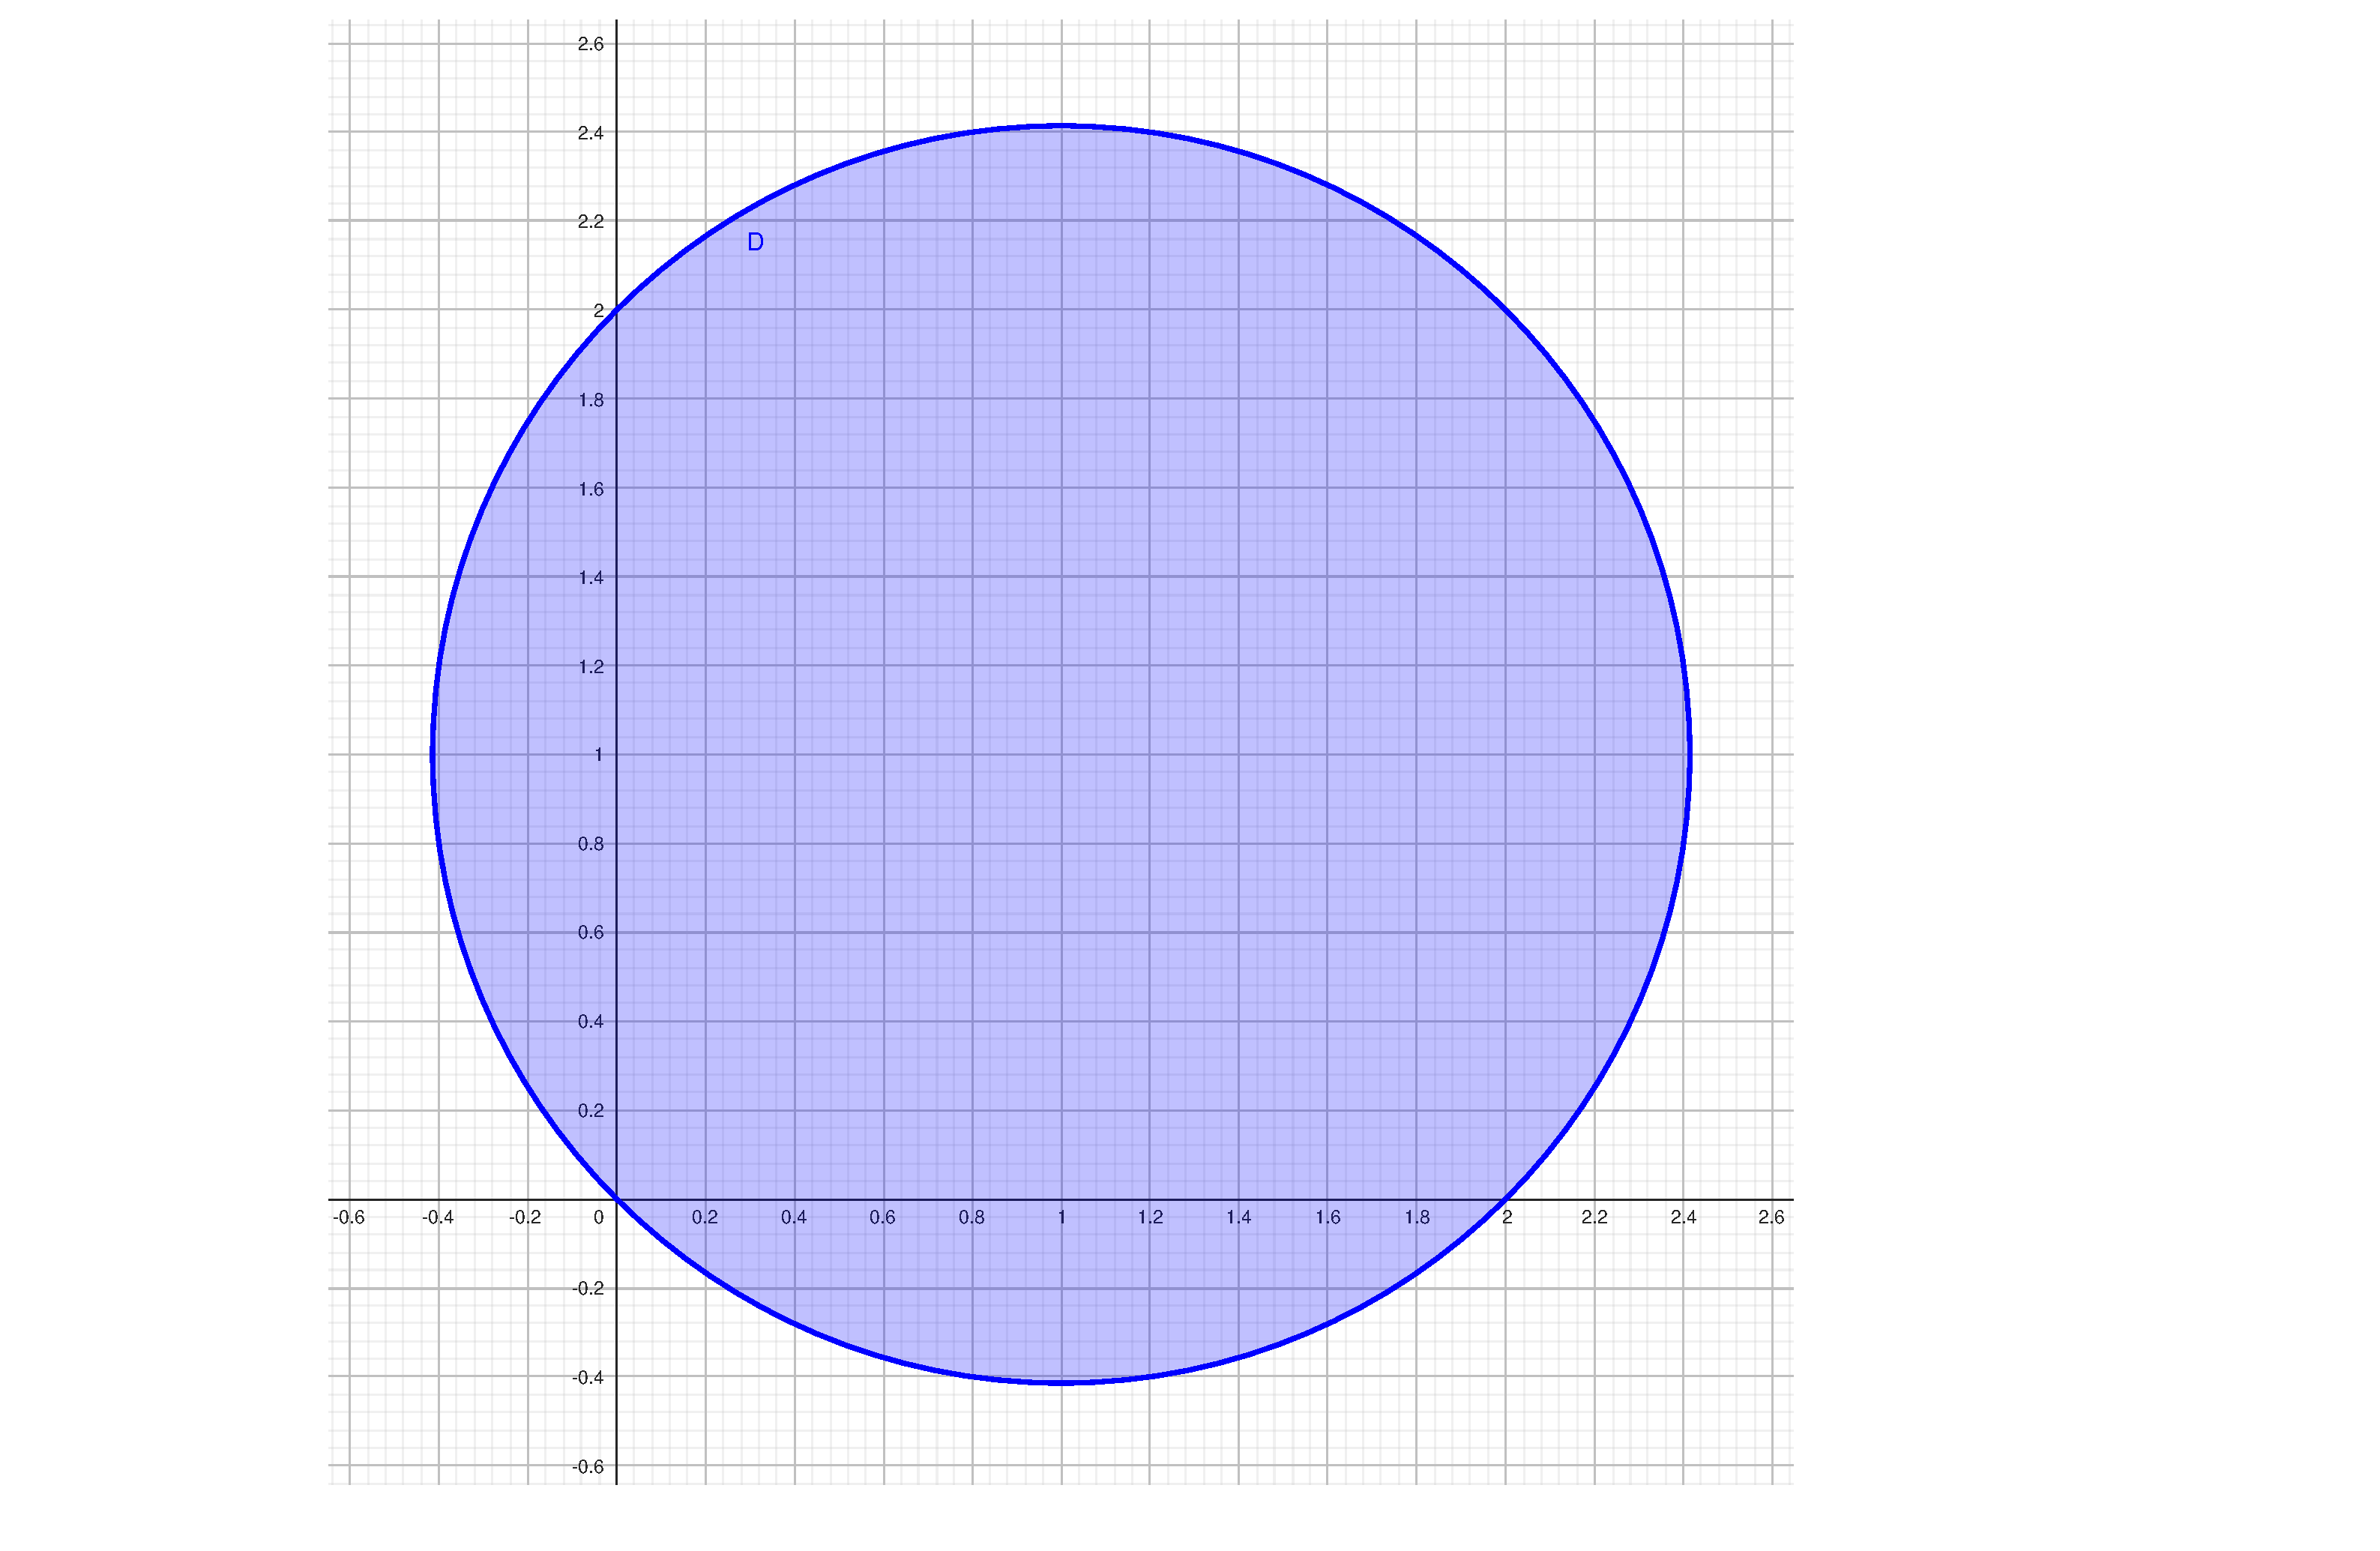
\includegraphics[width=\textwidth]{img/grafico-ex3-esame1.pdf}
	\end{figure}
	\begin{itemize}
		\item Limitato o illimitato? L'insieme è limitato, possibile vederlo dalla figura (poco da motivare);
		
		\item Aperto o chiuso? L'insieme non è né aperto né chiuso a causa della condizione $x \ne 0$ che impedisce di avere tutti i punti della frontiera;
		
		\item Connesso o sconnesso? L'insieme è sconnesso, possibile vederlo dalla figura e dalla condizione $x \ne 0$.
	\end{itemize}
	Si prosegue la risoluzione dell'esercizio risolvendo il punto $b$.
	
	
	\newpage

	\section{Esercizio 4 - Stabilire se una funzione è continua e parametrizzazioni}

	\subsection{Tipologie di esercizio 1}

	\subsubsection{Stabilire se una funzione è continua}

	Un \emph{evergreen} nell'esercizio 4 è la richiesta di stabilire se la funzione data è continua in un certo insieme. Il procedimento è il seguente; si estrae un esercizio dal tema d'esame del 15/09/2021, gruppo A: \textcolor{Green4}{\textbf{\emph{Stabilire se la funzione:}}
	\begin{equation*}
		f\left(x,y\right) = \begin{cases}
			\dfrac{y^{4}}{x^{2} + y^{4}} & \left(x,y\right) \ne \left(0,0\right) \\
			\\
			0	& \left(x,y\right) = \left(0,0\right)
		\end{cases}
	\end{equation*}
	\textbf{\emph{è continua in $\mathbb{R}^{2}$.}}}\newline

	\noindent
	La soluzione di questo esercizio, il più delle volte, è affermare che la funzione non è continua nell'insieme dato. Tuttavia, talvolta non è così scontato ed è necessario dimostrare il motivo della risposta.\newline
	
	\noindent
	Il \textbf{primo passo}, banale e al 90\% verificabile visivamente, è verificare che la funzione sia definita nel punto $\left(0,0\right)$. Infatti, per stabilire se la funzione è continua in $\mathbb{R}^{2}$, è \underline{necessario} che sia continua nel punto $\left(0,0\right)$.

	In questo caso, l'esercizio afferma che nel caso in cui $x$ e $y$ siano zero $\left(x,y\right) = \left(0,0\right)$, la funzione abbia risultato $0$. Per cui, la funzione è definita.\newline

	\noindent
	Il \textbf{secondo passo} è verificare che esista il limite con $x$ che tende a zero e con $y$ che tende a zero. Nel caso in cui sia $\infty$, è possibile affermare che la funzione non è continua facendo vedere i calcoli del limite. In questo caso:
	\begin{equation*}
		\begin{array}{rcl}
			\displaystyle\lim_{x \rightarrow 0} f\left(x,0\right) &=& \dfrac{0^{4}}{x^{2} + 0^{4}} = \dfrac{0}{x^{2}} = 0 \\ [1.5em]
			\displaystyle\lim_{y \rightarrow 0} f\left(0,y\right) &=& \dfrac{y^{4}}{0^{2} + y^{4}} = \dfrac{y^{4}}{y^{4}} = 1
		\end{array}
	\end{equation*}
	I limiti non coincidono, per cui è possibile affermare che la funzione non è continua nell'origine $\left(0,0\right)$, ovvero i limite di $f$ per $\left(x,y\right) \rightarrow \left(0,0\right)$ non esiste. Quindi, $f$ non è continua in $\mathbb{R}^{2}$.\newline

	\noindent
	Per completezza, si presenta un esercizio in cui una funzione è continua per capire come comportarsi. Si estrae un esercizio dal tema d'esame del 01/03/2022: \textcolor{Green4}{\textbf{\emph{Stabilire se la funzione:}}
	\begin{equation*}
		f\left(x,y\right) = \begin{cases}
			\dfrac{\left(x-1\right)\left(y-2\right)}{\sqrt{\left(x-1\right)^{2} + \left(y-2\right)^{2}}} & \left(x,y\right) \ne \left(1,2\right) \\
			\\
			0	& \left(x,y\right) = \left(1,2\right)
		\end{cases}
	\end{equation*}
	\textbf{\emph{è continua in $\mathbb{R}^{2}$.}}}\newpage

	\noindent
	Il \textbf{primo passo} è verificare che la funzione sia definita in $\left(1,2\right)$. In questo caso lo è, quindi si passa avanti.\newline

	\noindent
	Il \textbf{secondo passo} è verificare i limiti con il punto $\left(1,2\right)$:
	\begin{equation*}
		\begin{array}{rcl}
			\displaystyle\lim_{x \rightarrow 1} f\left(x,2\right) &=& \dfrac{\left(x-1\right)\left(2-2\right)}{\sqrt{\left(x-1\right)^{2} + \left(2-2\right)^{2}}} \\ [2em]
			&=& \dfrac{0}{\sqrt{\left(x-1\right)^{2}}} \\ [2em]
			&=& 0 \\ [2em]
			\displaystyle\lim_{y \rightarrow 2} f\left(1,y\right) &=& \dfrac{\left(1-1\right)\left(y-2\right)}{\sqrt{\left(1-1\right)^{2} + \left(y-2\right)^{2}}} \\ [2em]
			&=& \dfrac{0}{\sqrt{\left(y-2\right)^{2}}} \\ [2em]
			&=& 0
		\end{array}
	\end{equation*}
	I due limiti esistono e hanno lo stesso risultato. Per essere certi che la funzione sia continua, è necessario un \textbf{terzo passo}, ovvero:
	\begin{equation*}
		\displaystyle\lim_{x \rightarrow x_{0}} f\left(x\right) = f\left(x_{0}\right)
	\end{equation*}
	Dato che il limite esiste ed è uguale a zero per $\left(1,2\right)$, nel caso di $f\left(1,2\right)$, si continua ad avere il valore $0$. Quindi, la funzione è continua.\newpage

	\subsubsection{Variante (rara) - Stabilire se una funzione è continua}

	Nell'esame del 03/03/2023 è stata fatta una richiesta diversa dal solito. È stato chiesto di stabilire un valore $k$ tale che la funzione risulti continua nell'origine: \textcolor{Green4}{\textbf{\emph{Si consideri la funzione:}}
	\begin{equation*}
		f\left(x,y\right) = \begin{cases}
			\dfrac{x^{2} + y^{2}}{x^{2} + xy + y^{2}}	& \left(x,y\right) \ne \left(0,0\right) \\
			k	& \left(x,y\right) = \left(0,0\right)
		\end{cases}
	\end{equation*}
	\textbf{\emph{Esiste un valore di $k \in \mathbb{R}$ tale che $f$ risulti continua nell'origine?}}}\newline

	\noindent
	Ipotizzando di muoversi lungo la retta per l'origine con $x \ne 0$, la funzione verrebbe riscritta come:
	\begin{equation*}
		f\left(x,mx\right) = \dfrac{x^{2} + m^{2}x^{2}}{x^{2} + mx^{2} + m^{2}x^{2}} = \dfrac{x^{2}\left(1+m^{2}\right)}{x^{2}\left(1 + m + m^{2}\right)} = \dfrac{1 + m^{2}}{1 + m + m^{2}}
	\end{equation*}
	Si vede anche ad occhio, che il limite della funzione $f\left(x,mx\right)$ con $x$ che tende a zero ($x \rightarrow 0$) dipende dal fattore $m$. Dunque è possibile concludere che tale limite non esiste:
	\begin{equation*}
		\displaystyle\lim_{\left(x,y\right) \rightarrow \left(0,0\right)} f\left(x,y\right)
	\end{equation*}
	Per cui, è possibile concludere che per nessun valore di $k$ la funzione $f$ è continua in $\left(0,0\right)$.\newpage

	\subsubsection{Dimostrazione di una disuguaglianza e di un limite (Teorema del confronto)}

	Nell'esame del 22/07/2021 è stato richiesto di eseguire dei calcoli insoliti rispetto alle classiche richieste degli esercizi: \textcolor{Green4}{\textbf{\emph{Dimostrare che:}}
	\begin{equation*}
		x^{2} |y| \le \dfrac{1}{2}\left(x^{4} + y^{2}\right) \hspace{2em} \text{per ogni } \left(x,y\right) \in \mathbb{R}^{2}
	\end{equation*}
	\textbf{\emph{e utilizzare la precedente disuguaglianza per verificare che:}}
	\begin{equation*}
		\displaystyle\lim_{\left(x,y\right) \rightarrow \left(0,0\right)} \dfrac{x^{3} y}{x^{4} + y^{2}} = 0
	\end{equation*}}\:\newline

	\noindent
	Il \textbf{primo passo} è dimostrare che vale la disuguaglianza mostrata. Per farlo, è necessario verificare che tutte le espressioni siano maggiore o uguale a zero, ovvero:
	\begin{equation*}
		\begin{array}{rcl}
			x^{2}|y| &\le& \dfrac{1}{2}\left(x^{4} + y^{2}\right) \\ [1em]
			2 \cdot x^{2}|y| &\le& \dfrac{1}{\cancel{2}}\left(x^{4} + y^{2}\right) \cdot \cancel{2} \\ [1em]
			2 x^{2}|y| &\le& \left(x^{4} + y^{2}\right) \\ [1em]
			-x^{4} + 2 x^{2}|y| &\le& y^{2} \\ [1em]
			-x^{4} + 2 x^{2}|y| - y^{2} &\le& 0 \\ [1em]
			x^{4} - 2 x^{2}|y| + y^{2} &\ge& 0 \\ [1em]
			\left(x^{2} - |y|\right)^{2} &\ge& 0 \\ [1em]
		\end{array}
	\end{equation*}
	Disuguaglianza verificata. Infatti, anche se ci fosse un numero negativo, l'elevazione al quadrato la farebbe tornare positiva. Al massimo l'espressione può essere zero, ma anche in tal caso l'espressione è ammessa. Quindi, è possibile concludere affermando che l'espressione risulta non negativa per ogni $\left(x,y\right) \in \mathbb{R}^{2}$.\newline
	
	\noindent
	Il \textbf{secondo passo} è utilizzare la disuguaglianza per verificare il limite. Si utilizza il teorema del confronto\footnote{\href{https://www.youmath.it/lezioni/analisi-matematica/limiti-continuita-e-asintoti/1562-teorema-dei-dei-carabinieri.html}{Link alla fonte di YouMath in cui ci sono esempi}}, che afferma: \emph{se $\left\{a_{n}\right\},\left\{b_{n}\right\},\left\{c_{n}\right\}$ sono tre successioni di numeri tali che:}
	\begin{equation*}
		a_{n} \le b_{n} \le c_{n}
	\end{equation*}
	\emph{e se si ha:}
	\begin{equation*}
		\displaystyle\lim_{n \rightarrow \infty} a_{n} = \displaystyle\lim_{n \rightarrow \infty} c_{n} = l
	\end{equation*}
	\emph{allora anche:}
	\begin{equation*}
		\displaystyle\lim_{n \rightarrow \infty} b_{n} = l
	\end{equation*}\newpage

	\noindent
	Per applicarlo, si prende in considerazione l'argomento del limite, cioè $\frac{x^{3}y}{x^{4}+y^{2}}$, e si afferma che deve essere maggiore o uguale a zero:
	\begin{equation*}
		0 \le \left| \dfrac{x^{3}y}{x^{4}+y^{2}} \right|
	\end{equation*}
	Dato che l'esercizio chiede di utilizzare anche la disuguaglianza precedente, lo studente dovrebbe avere l'intuizione di notare che:
	\begin{equation*}
		x^{2} |y| \le \dfrac{1}{2}\left(x^{4} + y^{2}\right)
	\end{equation*}
	Corrisponde a:
	\begin{equation*}
		\begin{array}{rcl}
			x^{2} |y| &\le& \dfrac{1}{2}\left(x^{4} + y^{2}\right) \\ [1em]
			\dfrac{1}{x^{4} + y^{2}} \cdot x^{2} |y| &\le& \dfrac{1}{2} \cdot \cancel{\left(x^{4} + y^{2}\right)} \cdot \dfrac{1}{\cancel{x^{4} + y^{2}}} \\ [1em]
			\dfrac{x^{2} |y|}{x^{4} + y^{2}} &\le& \dfrac{1}{2}
		\end{array}
	\end{equation*}
	Di nuovo, se lo studente riesce ad avere l'intuizione, noterà che aggiungendo una $|x|$, è possibile ottenere $\frac{x^{3}y}{x^{4}+y^{2}}$:
	\begin{equation*}
		0 \le \left| \dfrac{x^{3}y}{x^{4}+y^{2}} \right| = |x| \cdot \dfrac{x^{2} |y|}{x^{4} + y^{2}} \le \dfrac{1}{2} \cdot |x|
	\end{equation*}
	Quindi, grazie al teorema del confronto:
	\begin{equation*}
		0 \le |x| \cdot \dfrac{x^{2} |y|}{x^{4} + y^{2}} \le \dfrac{1}{2} \cdot |x|
	\end{equation*}
	Basta verificare che i limiti esterni siano uguali per affermare che anche quello al centro sia uguale:
	\begin{equation*}
		\begin{array}{ll}
			\displaystyle\lim_{\left(x,y\right) \rightarrow \left(0,0\right)} & 0 = 0 \\ [1em]
			\displaystyle\lim_{\left(x,y\right) \rightarrow \left(0,0\right)} & \dfrac{1}{2} \cdot |x| = 0
		\end{array}
	\end{equation*}
	Quindi, grazie al teorema del confronto, si afferma che:
	\begin{equation*}
		\displaystyle\lim_{\left(x,y\right) \rightarrow \left(0,0\right)} \dfrac{x^{3} y}{x^{4} + y^{2}} = 0
	\end{equation*}\newpage

	\subsubsection{Verificare l'esistenza di un limite in un punto}

	Un esercizio che è stato richiesto qualche volta, è la verifica dell'esistenza di un certo limite. Ovvero, viene fornita una funzione e un punto su cui verificare l'esistenza di tale limite. Si prenda d'esempio l'esame del 08/02/2022, gruppo A: \textcolor{Green4}{\textbf{\emph{Stabilire se la funzione:}}
	\begin{equation*}
		f\left(x,y\right) = \dfrac{y^{3} + |x-1|}{\left(x-1\right)^{2} + y^{2}}
	\end{equation*}
	\textbf{\emph{ammette limite per $\left(x,y\right) \rightarrow \left(1,0\right)$.}}}\newline

	\noindent
	Il \textbf{primo passo} è verificare con $x$ fissato:
	\begin{equation*}
		\begin{array}{rcl}
			\displaystyle\lim_{x \rightarrow 1} f\left(x, 0\right) &=& \dfrac{0^{3} + |x-1|}{\left(x-1\right)^{2} + 0^{2}} \\ [1.5em]
			&=& \dfrac{|x-1|}{\left(x-1\right)^{2}} \\ [1.5em]
			&\rightarrow& \text{Forma indeterminata } \frac{0}{0} \text{ quindi si usa Hopital} \\ [1em]
			&=& \dfrac{ \dfrac{d}{dx} |x-1|}{ \dfrac{d}{dx} \left(x-1\right)^{2}} \\ [2.5em]
			&\rightarrow& \text{Sapendo che } |x| = \sqrt{x^{2}} \\ [1em]
			&=& \dfrac{ \dfrac{d}{dx} \left(\sqrt{\left(x-1\right)^{2}}\right)}{ \dfrac{d}{dx} \left(x-1\right)^{2}} \\ [2.5em]
			&=& \dfrac{\dfrac{1}{2\sqrt{\left(x-1\right)^{2}}} \cdot \left(2x-2\right)}{ \dfrac{d}{dx} \left(x-1\right)^{2}} \\ [2.5em]
			&=& \dfrac{1}{2\left(x-1\right) \cdot 1} \\ [1.5em]
			&=& \dfrac{1}{2x - 2} \\ [1em]
			&=& \infty
		\end{array}
	\end{equation*}\newpage

	\noindent
	Il \textbf{secondo passo} è verificare con $y$ fissato:
	\begin{equation*}
		\begin{array}{rcl}
			\displaystyle\lim_{y \rightarrow 0} f\left(1, y\right) &=& \dfrac{y^{3} + |1-1|}{\left(1-1\right)^{2} + y^{2}} \\ [1.5em]
			&=& \dfrac{y^{3}}{y^{2}} \\ [1.5em]
			&=& y \\
			&=& 0
		\end{array}
	\end{equation*}
	Dato che il risultato dei due limiti è diverso, il limite nel punto $\left(1,0\right)$ non esiste.\newpage

	\subsection{Tipologie di esercizio 2}

	\subsubsection{Parametrizzazione retta tangente in un punto all'arco di ellisse}\label{par: parametrizzazione retta tangente in un punto all'arco di ellisse}

	Questa tipologia di esercizio si è presentata soltanto una volta, anche perché l'ellisse non è una figura semplice da trattare (parole testuali del professore). L'esame del 25/06/2021, gruppo A, chiedeva: \textcolor{Green4}{\textbf{\emph{Si trovi una parametrizzazione della retta tangente in $P\left(-2-\sqrt{3}, \frac{9}{2}\right)$ all'arco di ellisse di equazione:}}
	\begin{equation*}
		9x^{2} + 4y^{2} + 36x - 24y + 36 = 0
	\end{equation*}
	\textbf{\emph{che congiunge (nell'ordine) i punti $A\left(-2,6\right)$ e $B\left(-4,3\right)$.}}}\newline

	\noindent
	Quando ci si trova davanti ad un'ellisse o un'iperbole, è sempre conveniente utilizzare la tecnica del completamento dei quadrati. Questo perché la sua applicazione consente di ottenere direttamente la forma canonica dell'equazione cercata e di determinare i valori senza calcoli complessi\footnote{\href{https://youtu.be/a4ST5Kmjtxk}{Video tutorial di approfondimento}}.\newline

	\noindent
	Quindi, il \textbf{primo passo} è applicare il completamento dei quadrati:
	\begin{mdframed}
		Innanzitutto, la \textbf{prima operazione} dell'applicazione del completamento dei quadrati è il raggruppamento dei valori simili, ovverosia:
		\begin{equation*}
			\begin{array}{rcl}
				9x^{2} + 4y^{2} + 36x - 24y + 36 &=& 0 \\
				\left(9x^{2} + 36x\right) + \left(4y^{2} - 24y\right) + 36 &=& 0
			\end{array}
		\end{equation*}
		La \textbf{seconda operazione} è prendere in considerazione i termini con le $x$, e poi quelli con le $y$, e cercare un quadrato. Ovvero sia un valore $c$ tale per cui il $\Delta$ (nella formula del calcolo di un'equazione di secondo grado $\Delta = b^{2} - 4 \cdot a \cdot c$) sia uguale a zero:
		\begin{equation*}
			\begin{array}{rcl}
				9x^{2} + 36x &\longrightarrow& 36^{2} - 4 \cdot 9 \cdot c = 0 \\
				&& 36^{2} - 36c = 0 \\
				&& c = 36 \\ [1em]
				4y^{2} - 24y &\longrightarrow& 24^{2} - 4 \cdot 4 \cdot c = 0 \\
				&& 24^{2} - 16c = 0 \\
				&& c = 36
			\end{array}
		\end{equation*}
		\underline{Suggerimento}: per trovare tale valore, basta risolvere la banale equazione $b^{2} - 4 \cdot a \cdot c = 0$ con $c$ incognita e $a,b$ termini noti.\newpage

		\noindent
		La \textbf{terza operazione} è riscrivere l'equazione con i nuovi valori $c$, ma per lasciare invariata l'equazione è necessario annullarli, ovvero scrivere $c-c$ (nessun problema, con manipolazioni algebriche si riuscirà ad evitare di ritornare al punto di inizio):
		\begin{equation*}
			\left(9x^{2} + 36x + 36 - 36\right) + \left(4y^{2} - 24y + 36 - 36\right) + 36 = 0
		\end{equation*}
		Le manipolazioni algebriche riguardano $9x^{2} + 36x + 36$ e $4y^{2} - 24y + 36$. Ovvero, si riscrivono le due espressioni come quadrati!
		\begin{equation*}
			\begin{array}{rcl}
				9x^{2} + 36x + 36 &\longrightarrow& 9\left(x+2\right)^{2} \\
				4y^{2} - 24y + 36 &\longrightarrow& 4\left(y-3\right)^{2} \\
			\end{array}
		\end{equation*}
		E si riscrive l'equazione generale:
		\begin{equation*}
			9\left(x+2\right)^{2} - 36 + 4\left(y-3\right)^{2} - 36 + 36 = 0
		\end{equation*}
		Banali semplificazioni algebriche:
		\begin{equation*}
			\begin{array}{rcl}
				9\left(x+2\right)^{2} \cancel{- 36} + 4\left(y-3\right)^{2} - 36 \cancel{+ 36} &=& 0 \\ [1em]
				\dfrac{1}{36} \cdot \cancel{9}\left(x+2\right)^{2} + \cancel{4}\left(y-3\right)^{2} &=& \cancel{36} \cdot \dfrac{1}{\cancel{36}}  \\ [1em]
				\dfrac{\left(x+2\right)^{2}}{4} + \dfrac{\left(y-3\right)^{2}}{9} &=& 1
			\end{array}
		\end{equation*}
		Quest'ultima equazione corrisponde all'equazione canonica dell'ellisse.	
	\end{mdframed}

	\noindent
	Il \textbf{secondo passo} è la parametrizzazione\footnote{\href{https://www.youmath.it/forum/analisi-2n/70602-parametrizzazione-di-unellisse.html}{Approfondimento teorico - Parametrizzazione di un'ellisse}} vera e propria. La parametrizzazione di un'ellisse prevede l'utilizzo delle coordinate ellittiche\footnote{\href{https://www.youmath.it/forum/analisi-2n/7786-coordinate-ellittiche.html}{Approfondimento teorico - Coordinate ellittiche}}. Tali coordinate, che non fanno riferimento solo all'ellisse, sono ottenibili nel seguente modo:
	\begin{equation*}
		\dfrac{\left(x-x_{0}\right)^{2}}{a^{2}} + \dfrac{\left(y-y_{0}\right)^{2}}{b^{2}} = 1 \longrightarrow
		\begin{cases}
			x = x_{0} + a \rho \cos\left(\theta\right) \\
			y = y_{0} + b \rho \sin\left(\theta\right)
		\end{cases}
	\end{equation*}
	Quindi, nel nostro caso si ha:
	\begin{equation*}
		\dfrac{\left(x+2\right)^{2}}{4} + \dfrac{\left(y-3\right)^{2}}{9} = 1 \longrightarrow
		\begin{cases}
			x = -2 + 2 \cos\left(t\right) \\
			y = 3 + 3 \sin\left(t\right)
		\end{cases}
	\end{equation*}\newpage

	\noindent
	Il \textbf{terzo passo} è descrivere la congiunzione tra i punti $A$ e $B$ (in questo ordine). Per farlo, basta semplicemente sostituire nel sistema prima il punto $A$ e successivamente il punto $B$:
	\begin{gather*}
		A = \begin{cases}
			-2 = -2 + 2 \cos\left(t\right) \\
			6 = 3 + 3 \sin\left(t\right)
		\end{cases}
		\rightarrow
		\begin{cases}
			0 = 2 \cos\left(t\right) \\
			3 = 3 \sin\left(t\right)
		\end{cases}
		\rightarrow
		\begin{cases}
			0 = \cos\left(t\right) \\
			1 = \sin\left(t\right)
		\end{cases} \\
		\rightarrow
		\begin{cases}
			t = \arccos\left(0\right) = \frac{\pi}{2} \\
			t = \arcsin\left(1\right) = \frac{\pi}{2}
		\end{cases} \\
		\\
		B = \begin{cases}
			-4 = -2 + 2 \cos\left(t\right) \\
			3 = 3 + 3 \sin\left(t\right)
		\end{cases}
		\rightarrow
		\begin{cases}
			-2 = 2 \cos\left(t\right) \\
			0 = 3 \sin\left(t\right)
		\end{cases}
		\rightarrow
		\begin{cases}
			-1 = \cos\left(t\right) \\
			0 = \sin\left(t\right)
		\end{cases} \\
		\rightarrow
		\begin{cases}
			t = \arccos\left(-1\right) = \pi \\
			t = \arcsin\left(0\right) = 0 = \pi
		\end{cases}
	\end{gather*}
	Quindi, la parametrizzazione finale è:
	\begin{equation*}
		\gamma : \left[\dfrac{\pi}{2}, \pi\right] \rightarrow \mathbb{R}^{2}, \hspace{2em} \gamma\left(t\right) = \left(-2+2\cos\left(t\right), \: 3 + 3\sin\left(t\right)\right)
	\end{equation*}
	Il \textbf{quarto passo} è trovare la parametrizzazione della retta tangente passante nel punto $P\left(-2-\sqrt{3}, \frac{9}{2}\right)$. Per farlo, è necessario sostituire il punto $P$ nella parametrizzazione dell'ellisse, e successivamente fare la derivata per trovare la tangente:
	\begin{gather*}
		\begin{cases}
			-2-\sqrt{3} = -2 + 2\cos\left(t\right) \\
			\\
			\dfrac{9}{2} = 3 + 3\sin\left(t\right)
		\end{cases}
		\rightarrow
		\begin{cases}
			-\sqrt{3} = 2\cos\left(t\right) \\
			\\
			\dfrac{3}{2} = 3\sin\left(t\right)
		\end{cases}
		\rightarrow
		\begin{cases}
			-\dfrac{\sqrt{3}}{2} = \cos\left(t\right) \\
			\\
			\dfrac{\cancelto{1}{3}}{\cancelto{2}{6}} = \sin\left(t\right)
		\end{cases} \\
		\rightarrow
		\begin{cases}
			t = \arccos\left(-\dfrac{\sqrt{3}}{2}\right) = \dfrac{5\pi}{6} \\
			\\
			t = \arcsin\left(\dfrac{1}{2}\right) = \dfrac{5\pi}{6}
		\end{cases}\\
		\\
		\gamma\left(\dfrac{5\pi}{6}\right) = \left(P\right) = \left(-2-\sqrt{3}, \dfrac{9}{2}\right) \\
		\\
		\gamma'\left(\dfrac{5\pi}{5}\right) \rightarrow \begin{cases}
			x' = \frac{d}{dx} -2 + 2 \cos\left(t\right) \\
			y' = \frac{d}{dy} 3 + 3 \sin\left(t\right)
		\end{cases}
		\rightarrow
		\begin{cases}
			x' = - 2\sin\left(t\right) & = -2\sin\left(\dfrac{5\pi}{6}\right) = -1 \\
			\\
			y' = \phantom{-}3\cos\left(t\right)   & = \phantom{-}3\cos\left(\dfrac{5\pi}{6}\right) = -\dfrac{3\sqrt{3}}{2}
		\end{cases}
	\end{gather*}\newpage

	\noindent
	Il \textbf{quinto passo} è scrivere la retta finale tangente al punto $P$. Per farlo, basta scrivere il sistema (parametrizzazione) con le due coordinate $x$ e $y$ in funzione di $t$, e come valori si hanno: i punti di $P$ $+$ i punti trovati grazie alla derivata $\times t$.
	\begin{equation*}
		\begin{array}{rcl}
			\text{Punto }P	&\longrightarrow& P\left(-2-\sqrt{3}, \: \dfrac{9}{2}\right) \\ [1.5em]
			\text{Soluzioni derivata }\gamma'\left(\dfrac{5\pi}{6}\right) &\longrightarrow& \gamma'\left(\dfrac{5\pi}{6}\right) = \left(-1, \: -\dfrac{3\sqrt{3}}{2}\right) \\ [1.5em]
			\begin{cases}
				x\left(t\right) = -2-\sqrt{3} + \left(-1\right) \cdot t \\
				\\
				y\left(t\right) = \dfrac{9}{2} + \left(-\dfrac{3\sqrt{3}}{2}\right) \cdot t
			\end{cases} & \longrightarrow & \begin{cases}
				x\left(t\right) = -2-\sqrt{3} - t \\
				\\
				y\left(t\right) = \dfrac{9}{2} - \dfrac{3\sqrt{3}}{2} t
			\end{cases} t \in \mathbb{R}
		\end{array}
	\end{equation*}\:\newline

	\longline

	\subsubsection{Trovare l'equazione al piano tangente}

	Negli esami del 15/09/2021 e del 22/07/2021 è stato chiesto questo esercizio. La risoluzione si può trovare a pagina:~\pageref{par: trovare l'equazione al piano tangente}.\newpage

	\subsubsection{Determinare le equazioni parametriche della retta tangente all'arco di curva nel punto $P$}

	Questa tipologia di esercizio è molto richiesta. La sua risoluzione non è complessa se è chiaro lo svolgimento dell'esercizio sulla parametrizzazione della retta tangente di un punto all'arco di ellisse (pagina~\pageref{par: parametrizzazione retta tangente in un punto all'arco di ellisse}). Si prenda in considerazione l'esame del 23/11/2021: \textcolor{Green4}{\textbf{\emph{Si consideri l'arco di curva:}}
	\begin{equation*}
		\gamma : \left[0, \dfrac{\pi}{2}\right] \rightarrow \mathbb{R}^{2}, \hspace{2em} t \mapsto \left(\cos^{3}\left(t\right), \sin^{3}\left(t\right)\right)
	\end{equation*}
	\textbf{\emph{Determinare le equazioni parametriche della retta tangente a $\gamma$ nel punto $P\left(\frac{3\sqrt{3}}{8}, \frac{1}{8}\right)$.}}}\newline

	\noindent
	Il \textbf{primo passo} è sostituire il valore del punto dato, ovvero $P\left(\frac{3\sqrt{3}}{8}, \frac{1}{8}\right)$, all'interno della parametrizzazione dell'arco di curva al posto di $x$ e $y$:
	\begin{equation*}
		\begin{cases}
			\dfrac{3\sqrt{3}}{8} = \cos^{3}\left(t\right) \\
			\\
			\dfrac{1}{8} = \sin^{3}\left(t\right)
		\end{cases}
		\rightarrow
		\begin{cases}
			\sqrt[3]{\dfrac{3\sqrt{3}}{8}} = \sqrt[3]{\cos^{3}\left(t\right)} \\
			\\
			\sqrt[3]{\dfrac{1}{8}} = \sqrt[3]{\sin^{3}\left(t\right)}
		\end{cases}
		\rightarrow
		\begin{cases}
			\dfrac{\sqrt{3}}{2} = \cos\left(t\right) \\
			\\
			\dfrac{1}{2} = \sin\left(t\right)
		\end{cases}
		\rightarrow
		\begin{cases}
			t = \dfrac{\pi}{6} \\
			\\
			t = \dfrac{\pi}{6}
		\end{cases}
	\end{equation*}
	Il \textbf{secondo passo} è eseguire la derivata dell'arco di curva, ovvero della sua parametrizzazione, con argomento $\frac{\pi}{6}$:
	\begin{equation*}
		\begin{array}{rcl}
			\gamma\left(\dfrac{\pi}{6}\right) &=& \left(\dfrac{3\sqrt{3}}{8}, \: \dfrac{1}{8}\right) \\ [1em]
			\gamma'\left(\dfrac{\pi}{6}\right) &=& \left(-3 \cos^{2}\left(t\right) \cdot \sin\left(t\right), \: 3 \sin^{2}\left(t\right) \cos\left(t\right)\right) \\ [1em]
			&=& \left(-3 \cos^{2}\left(\dfrac{\pi}{6}\right) \cdot \sin\left(\dfrac{\pi}{6}\right), \: 3 \sin^{2}\left(\dfrac{\pi}{6}\right) \cos\left(\dfrac{\pi}{6}\right)\right) \\ [1em]
			&=& \left(-3 \cdot \dfrac{3}{4} \cdot \dfrac{1}{2}, \: 3 \cdot \dfrac{1}{4} \cdot \dfrac{\sqrt{3}}{2} \right) \\ [1.5em]
			&=& \left(-\dfrac{9}{8}, \: - \dfrac{3\sqrt{3}}{8}\right)
		\end{array}
	\end{equation*}
	Il risultato della derivata rappresenta la direzione della retta tangente in $P$ alla curva $\gamma'\left(\frac{\pi}{6}\right)$.\newline

	\noindent
	Il \textbf{terzo e ultimo passo} è scrivere le equazioni parametriche della retta, ricordando la formula utilizzata nel paragrafo~\ref{par: parametrizzazione retta tangente in un punto all'arco di ellisse}, ovverosia: \emph{scrivere il sistema (parametrizzazione) con le due coordinate $x$ e $y$ in funzione di $t$, e come valori si hanno: i punti di $P$ $+$ i punti trovati grazie alla derivata $\times t$}.
	\begin{equation*}
		\begin{cases}
			x = \dfrac{3\sqrt{3}}{8} -\dfrac{9}{8} \cdot t \\
			\\
			y = \dfrac{1}{8} +\dfrac{3\sqrt{3}}{8} \cdot t
		\end{cases} t \in \mathbb{R}
	\end{equation*}\newpage

	\noindent
	Negli ultimi anni, in particolare nel 2023, in due esami si è presentata anche una nuova richiesta: \underline{calcolare la lunghezza} dell'arco. Questo esercizio si risolve tramite una formula e l'utilizzo di un integrale. Si estrae dall'esame del 03/03/2023 l'esercizio: \textcolor{Green4}{\textbf{\emph{Si consideri l'arco di curva parametrizzato da:}}
	\begin{equation*}
		\gamma\left(t\right) = \left(t - \sin\left(t\right), 1 - \cos\left(t\right)\right), \hspace{1em} t \in \left[0,2\pi\right]
	\end{equation*}
	\textbf{\emph{Calcolare la lunghezza dell'arco e scrivere le equazioni parametriche della retta tangente alla curva nel punto $P\left(\frac{\pi}{2} -1, \: 1\right)$.}}}\newline

	\noindent
	Il \textbf{primo passo}, utile anche al calcolo delle equazioni parametriche della retta, è calcolare la derivata della parametrizzazione della curva:
	\begin{equation*}
		\begin{array}{rcl}
			\gamma\left(t\right) &=& \left(t-\sin\left(t\right), 1-\cos\left(t\right)\right) \\ [.5em]
			\gamma'\left(t\right) &=& \left(1-\cos\left(t\right), \: \sin\left(t\right)\right) \\ [1em]
			&=& \begin{cases}
				x'\left(t\right) = 1-\cos\left(t\right) \\
				y'\left(t\right) = \sin\left(t\right)
			\end{cases}
		\end{array}
	\end{equation*}
	Il \textbf{secondo passo} è calcolare la lunghezza\footnote{\href{https://www.youmath.it/lezioni/analisi-due/varie/716-come-calcolare-la-lunghezza-di-una-curva.html}{Link di approfondimento}} dell'arco tramite la seguente formula:
	\begin{equation*}
		L\left(\mathcal{L}\right) = \displaystyle\int_{a}^{b} || \gamma'\left(t\right) || \: \mathrm{d}t = \displaystyle\int_{a}^{b} \sqrt{x'\left(t\right)^{2} + y'\left(t\right)^{2}} \: \mathrm{d}t
	\end{equation*}
	Ovvero, si deve calcolare l'integrale dal punto di partenza $a$ al punto di destinazione $b$, della derivata al quadrato dell'equazione $x$ e $y$ della parametrizzazione, tutto sotto radice (più facile a farsi che a dirsi). Quindi, si vanno a sostituire i valori trovati, ricordando che il punto $a,b$ è il punto in cui è definito $t$, ovvero $t \in \left[0,2\pi\right]$:
	\begin{equation*}
		\begin{array}{rcl}
			L\left(\mathcal{L}\right) &=& \displaystyle\int_{0}^{2\pi} \sqrt{\left(1-\cos\left(t\right)\right)^{2} + \left(\sin\left(t\right)\right)^{2}} \: \mathrm{d}t \\ [1em]
			&=& \displaystyle\int_{0}^{2\pi} \sqrt{1 - \cos\left(t\right) - \cos\left(t\right) + \cos^{2}\left(t\right) + \sin^{2}\left(t\right)} \: \mathrm{d}t \\ [1em]
			&=& \displaystyle\int_{0}^{2\pi} \sqrt{1 - 2\cos\left(t\right) + \cos^{2}\left(t\right) + \sin^{2}\left(t\right)} \: \mathrm{d}t \\ [1em]
			&=& \displaystyle\int_{0}^{2\pi} \sqrt{1 - 2\cos\left(t\right) + 1} \: \mathrm{d}t \\ [1em]
			&=& \displaystyle\int_{0}^{2\pi} \sqrt{2 - 2\cos\left(t\right)} \: \mathrm{d}t \\ [1em]
			&=& 8
		\end{array}
	\end{equation*}
	La lunghezza dunque è stata trovata. Il risultato dell'integrale è possibile calcolarlo con una calcolatrice scientifica. L'esercizio continuerebbe calcolando le equazioni della retta tangente: si sostituisce il punto $P$ nel sistema così da ottenere l'angolo $t$; si sostituisce l'angolo $t$ trovato nella derivata $\gamma'$; si conclude scrivendo le equazioni della retta tangente utilizzando la formula $P + \gamma'\left(\text{angolo }\pi\right) \cdot t$.\newpage

	\noindent
	Si conclude questa tipologia di esercizio (tra i più gettonati) presentando due richieste particolari:
	\begin{itemize}
		\item Esame del 15/07/2022: \textcolor{Green4}{\textbf{\emph{Si consideri l'arco di curva $\mathcal{L}$ parametrizzato da:}}
		\begin{equation*}
			\gamma\left(t\right) = \left(13\sin\left(2t\right), \: 12\cos\left(2t\right), \: 5\cos\left(2t\right)\right), \hspace{1em} t \in \left[0, \pi\right]
		\end{equation*}
		\textbf{\emph{Calcolare la lunghezza di $\mathcal{L}$ e verificare che in ogni punto $P \in \mathcal{L}$ la retta tangente alla curva è perpendicolare alla retta $OP$ ($O$ è l'origine del sistema di riferimento).}}}

		Tralasciando il metodo per il calcolo della lunghezza, che banalmente corrisponde al calcolo delle derivate di $\gamma\left(t\right)$ e alla formula con l'integrale (pagina precedente), in questo esame è richiesto di verificare che la retta tangente in ogni punto $P$ della curva è perpendicolare alla retta $OP$. Il \textbf{primo e unico passo} è dimostrare che $\gamma\left(t\right) \cdot \gamma'\left(t\right) = 0$ per ogni $t \in \left[0,\pi\right]$. Quindi, si va a sostituire:
		\begin{equation*}
			\begin{array}{rcl}
				\gamma\left(t\right) &=& \left(13\sin\left(2t\right), \: 12\cos\left(2t\right), \: 5\cos\left(2t\right)\right) \\
				\gamma'\left(t\right) &=& \left(26\cos\left(2t\right), \: -24\sin\left(2t\right), \: -10\sin\left(t\right)\right) \\
				\gamma\left(t\right) \cdot \gamma'\left(t\right) &=& 338\sin\left(2t\right)\cos\left(2t\right) - 288\sin\left(2t\right)\cos\left(2t\right) - 50 \sin\left(2t\right)\cos\left(2t\right) \\
				&=& 0
			\end{array}
		\end{equation*}
		Ed è immediato il risultato. Ovvero, che la moltiplicazione dia risultato zero $\forall t \in \left[0,\pi\right]$.

		\item Esame del 23/06/2022 (A): \textcolor{Green4}{\textbf{\emph{Si consideri l'arco di curva $\mathcal{L}$ parametrizzato da:}}
		\begin{equation*}
			\gamma\left(t\right) = \left(e^{t}, \: e^{-t}, \: t\sqrt{2}\right), \hspace{2em} t\in\left[0, \ln\left(5\right)\right]
		\end{equation*}
		\textbf{\emph{Calcolare la lunghezza di $\mathcal{L}$ (tenere in conto che $e^{t} \cdot e^{-t} = 1$) e stabilire se la retta tangente in $P\left(3, \frac{1}{3}, \sqrt{2}\ln\left(3\right)\right)$ all'arco $\mathcal{L}$ passa anche per il punto $Q\left(6,0,\sqrt{2}\left(1+\ln\left(3\right)\right)\right)$.}}}

		Tralasciando anche qui il calcolo della lunghezza (si rimanda alla pagina precedente) e il calcolo per verificare se la retta è tangente in $P$, il calcolo per verificare se l'arco di curva parametrizzato passa per il punto $Q$ è banale.

		Il \textbf{primo e unico passo} è sostituire i valori del punto $Q$ all'interno della parametrizzazione della retta tangente:
		\begin{enumerate}
			\item Calcolo parametrizzazione della retta tangente: sostituisco i punti di $P$ nel sistema di $\gamma\left(t\right)$ e ottengo la $t$;
		
			\item Calcolo la lunghezza: derivo $\gamma\left(t\right)$, applico l'integrale definito da $0$ a $\ln\left(5\right)$ ricordando di mettere sotto radice le derivate di $x,y,z$ al quadrato;\newpage
		
			\item Date le equazioni parametriche della retta tangente (trovata al punto 1):
			\begin{equation*}
				\begin{cases}
					x\left(t\right) = 3 + 3t \\
					\\
					y\left(t\right) = \dfrac{1}{3} - \dfrac{1}{3}t \\
					\\
					z\left(t\right) = \sqrt{2}\ln\left(3\right) + t\sqrt{2}
				\end{cases}
				t \in \mathbb{R}
			\end{equation*}
			Si può affermare che la retta passa per il punto $Q\left(6,0,\sqrt{2}\left(1+\ln\left(3\right)\right)\right)$, andando a sostituire i suoi punti nel sistema e calcolandosi $t$ (in questo caso $1$):
			\begin{equation*}
				\begin{cases}
					6 = 3 + 3t \\
					\\
					0 = \dfrac{1}{3} - \dfrac{1}{3}t \\
					\\
					\sqrt{2}\left(1+\ln\left(3\right)\right) = \sqrt{2}\ln\left(3\right) + t\sqrt{2}
				\end{cases}
				\longrightarrow
				\begin{cases}
					t = 1 \\
					t = 1 \\
					t = 1
				\end{cases}
			\end{equation*}
		\end{enumerate}
	\end{itemize}\newpage

	\subsubsection{Calcolare la pendenza della retta tangente (teorema di Dini)}

	Nell'esame del 22/07/2021 è stato richiesto di calcolare la pendenza di una retta. Questa richiesta insolita, è semplice da risolvere poiché basta applicare il teorema di Dini\footnote{\href{https://www.youmath.it/domande-a-risposte/view/1838-teorema-di-dini-help-me.html}{Link di approfondimento}}. L'esercizio estratto dal tema d'esame è: \textcolor{Green4}{\textbf{\emph{Sempre con $f$ definita come nel punto precedente, calcolare la pendenza della retta tangente in $\left(1,0\right)$ alla curva di equazione $f\left(x,y\right) = 0$.}}}\newline

	\noindent
	Al punto precedente veniva chiesto di determinare l'equazione del piano tangente al grafico di $f\left(x,y\right) = e^{x}y + \ln\left(x^{2} + y^{2}\right)$ nel punto $\left(1,0,f\left(1,0\right)\right)$. Si procede con la risoluzione del gradiente in modo rapido:\
	\begin{equation*}
		\begin{array}{rcl}
			f\left(x,y\right) &=& e^{x}y + \ln\left(x^{2} + y^{2}\right) \\ [1em]
			f\left(1,0\right) &=& e^{1} \cdot 0 + \ln\left(1^{2} + 0^{2}\right) = 0 \\ [1em]
			\dfrac{\partial f}{\partial x}\left(x,y\right) &=& e^{x}y + \dfrac{1}{x^{2} + y^{2}} \cdot \left(2x\right) \\ [1.5em]
			\dfrac{\partial f}{\partial x}\left(1,0\right) &=& e^{1}\cdot 0 + \dfrac{1}{1^{2} + 0^{2}} \cdot \left(2 \cdot 1\right) = 2 \\ [2em]
			\dfrac{\partial f}{\partial y}\left(x,y\right) &=& e^{x} + \dfrac{1}{x^{2} + y^{2}} \cdot \left(2y\right) \\ [1.5em]
			\dfrac{\partial f}{\partial y}\left(1,0\right) &=& e^{1} + \dfrac{1}{1^{2} + 0^{2}} \cdot \left(2 \cdot 0\right) = e \\ [2em]
			z &=& f\left(x_{0},y_{0}\right) + \dfrac{\partial f}{\partial x}\left(x_{0}, y_{0}\right)\left(x-x_{0}\right) + \dfrac{\partial f}{\partial y}\left(x_{0}, y_{0}\right)\left(y-y_{0}\right) \\ [1em]
			&=& 0 + 2\left(x-1\right) + ey \\
			&=& 2x -2 + ey
		\end{array}
	\end{equation*}
	Il \textbf{primo e unico passo} per l'applicazione del teorema di Dini, così da trovare la pendenza della retta tangente in $\left(1,0\right)$, è calcolare il rapporto tra le due derivate parziali valutate nel punto $\left(1,0\right)$:
	\begin{equation*}
		m = - \dfrac{\dfrac{\partial f}{\partial x}\left(1,0\right)}{\dfrac{\partial f}{\partial y}\left(1,0\right)} = - \dfrac{2}{e}
	\end{equation*}
	Attenzione che il valore meno appartiene alla formula del teorema di Dini e non è messo lì per caso.\newpage

	\section{Esercizio 5 - Studio dei massimi, minimi, punti critici e di sella di una funzione}
	
	\subsection{Tipologie di esercizio}

	\subsubsection{Verificare infinità dei punti stazionari di una funzione e trovare il punto di sella}\label{par: verificare infinità dei punti stazionari di una funzione e trovare il punto di sella}

	Questo esercizio è raro che venga chiesto dato che si presenta solo nell'esame del 25/06/2021(A). Tuttavia, il suo svolgimento non è complesso: \textcolor{Green4}{\textbf{\emph{Verificare che in $\mathbb{R}^{2}$ la funzione $f$ ha infiniti punti stazionari. Dimostrare che tra questi c'è un unico punto di sella.}}
	\begin{equation*}
		f\left(x,y\right) = xy^{2}
	\end{equation*}}
	Per verificare che i punti stazionari siano infiniti, basta semplicemente calcolare le derivate parziali rispetto $f$ e valutare le soluzioni che risolvono il sistema. Quindi, il \textbf{primo passo} è calcolare le derivate parziali di $f$:
	\begin{equation*}
		f\left(x,y\right) = xy^{2} \longrightarrow
		\begin{cases}
			\dfrac{\partial f}{\partial x}\left(x,y\right) = y^{2} \\
			\\
			\dfrac{\partial f}{\partial y}\left(x,y\right) = 2xy \\
		\end{cases}
	\end{equation*}
	I punti che risolvono il sistema sono $\left(x, 0\right)$, poiché y deve essere uguale a zero, mentre $x$ può essere qualsiasi valore ($x \in \mathbb{R}$) poiché verrà annullato dallo zero della $y$ ($2x \cdot 0$). Dato che $x$ può essere qualsiasi valore, è possibile affermare che i punti stazionari per $f$ sono infiniti!\newline

	\noindent
	Il \textbf{secondo passo} è trovare l'unico punto di sella (per approfondire il punto di sella, guardare il prossimo paragrafo). Per farlo sono necessarie alcune considerazioni. Infatti, con $x = 0$, nel punto $\left(0,0\right)$ si ha punto di sella (questo perché nell'intorno di $\left(0,0\right)$ la funzione $f\left(x,y\right)$ cambia di segno). Al contrario, nei casi in cui $x$ fosse $> 0$ o $< 0$, allora si  avrebbe rispettivamente un minimo locale e un massimo locale (che non sono punti di sella). Quest'ultima affermazione è vera poiché prendendo un intorno di $\left(0,y\right)$, nel primo caso si avrebbe la funzione $f\left(x,y\right) \ge 0$ e nel secondo caso si avrebbe la funzione $f\left(x,y\right) \le 0$.\newpage

	\subsubsection{Determinare valore di un parametro così da trovare un punto critico}\label{par: determinare valore di un parametro così da trovare un punto critico}

	Nell'esame del 22/07/2021 viene data una funzione e viene richiesto di calcolare un parametro $a$ così da ottenere un punto critico in un punto specifico. La sua risoluzione è semplice, infatti vale solo un punto.\newline
	\textcolor{Green4}{\textbf{\emph{Determinare il valore del parametro reale $a$ in modo che $f\left(x,y\right) = x - y^{2} + ax^{2}$ abbia un punto critico in $\left(-1, 0\right)$. Inoltre, classificare tale punto critico.}}}\newline

	\noindent
	Il \textbf{primo passo} è trovare tutti i punti critici della funzione così da poter affermare quale valore di $a$ è necessario. Per farlo, si utilizzano le derivate parziali sulla funzione $f\left(x,y\right)$:
	\begin{equation*}
		\begin{cases}
			\dfrac{\partial f}{\partial x} = 1 + 2ax	& \rightarrow x = -\dfrac{1}{2a} \\
			\\
			\dfrac{\partial f}{\partial y} = -2y		& \rightarrow y = 0 \\
		\end{cases}
	\end{equation*}
	La soluzione del sistema è: $\left(-\frac{1}{2a}, \: 0\right)$.\newline

	\noindent
	Il \textbf{secondo passo} è prendere in considerazione il punto critico richiesto, in questo caso $\left(-1, 0\right)$, e metterlo a sistema per estrarre la $a$:
	\begin{equation*}
		\begin{cases}
			-\dfrac{1}{2a} = -1 & \rightarrow a = \dfrac{1}{2} \\
			0 = 0 & \rightarrow \text{condizione già verificata } \textcolor{Green4}{\mathbf{\checkmark}}
		\end{cases}
	\end{equation*}
	Quindi, è possibile affermare che il punto critico $\left(-1,0\right) \iff a = \frac{1}{2}$.\newline

	\noindent
	Il \textbf{terzo passo} è necessario per classificare il punto critico. Per farlo, si sfrutta la matrice Hessiana\footnote{\href{https://www.youmath.it/lezioni/analisi-due/varie/1150-massimi-e-minimi-funzioni-due-variabili.html}{Link approfondimento teorico}}, ovvero una matrice costruita con le derivate parziali seconde. Andando a sostituire i valori del punto critico all'interno della matrice e andando a calcolare il determinante, è possibile stabilire se si tratta di un punto di massimo/minimo o di sella.
	\begin{equation*}
		\begin{array}{rcl}
			\text{Definizione teorica:} &\longrightarrow& H_{f}\left(x,y\right) = \begin{bmatrix}
				f_{xx}\left(x,y\right)	& f_{xy}\left(x,y\right) \\
				f_{yx}\left(x,y\right)	& f_{yy}\left(x,y\right)
			\end{bmatrix} \\
			\\
			\text{Calcolo dell'esercizio:} &\longrightarrow& H_{f}\left(x,y\right) = \begin{bmatrix}
				1	& 0 \\
				0	& -2
			\end{bmatrix} \\
			\\
			\text{Sostituzione valori:} &\longrightarrow& H_{f}\left(-1, 0\right) = \begin{bmatrix}
				1	& 0 \\
				0	& -2
			\end{bmatrix}
		\end{array}
	\end{equation*}
	Ovviamente si assume che la derivata parziale prima rispetto a $x$ sia con $a = \frac{1}{2}$, quindi $\frac{\partial f}{\partial x} = 1+x$. Si calcola il determinante:
	\begin{equation*}
		\det\left(H_{f}\left(-1, 0\right)\right) = 1 \cdot \left(-2\right) = -2
	\end{equation*}\newpage

	\noindent
	È possibile dunque affermare immediatamente che si tratta di un \underline{punto di sella}. Per capire con quale logica è stata presa questa scelta, si lascia un piccolo richiamo alla teoria del corso.

	\begin{table}[!htp]
		\begin{mdframed}
			\textbf{\emph{Richiamo alla teoria del corso}}\newline

			\noindent
			È possibile classificare i punti stazionari a seconda del risultato del determinante della matrice Hessiana e al valore della derivata parziale seconda:\newline

			\noindent
			\centering
			\begin{tabular}{@{} c | c | c @{}}
				\toprule
				Determinante & Derivata p. sec. & Definizione di $\left(x,y\right)$ \\
				\midrule
				$\det\left(H_{f}\left(x,y\right)\right) > 0$	& $\dfrac{\partial^{2} f}{\partial x^{2}}\left(x,y\right) > 0$	& Minimo locale \\ [1.5em]
				$\det\left(H_{f}\left(x,y\right)\right) > 0$	& $\dfrac{\partial^{2} f}{\partial x^{2}}\left(x,y\right) < 0$	& Massimo locale \\ [1.5em]
				$\det\left(H_{f}\left(x,y\right)\right) < 0$	& \ding{55}														& Punto di sella \\ [1em]
				$\det\left(H_{f}\left(x,y\right)\right) = 0$	& \ding{55}														& Poche informazioni \\
				\bottomrule
			\end{tabular}
			\vspace{1em}
		\end{mdframed}
	\end{table}\newpage

	\subsubsection{Determinare \underline{tutti} i punti critici di una funzione (con analisi della loro natura)}

	Determinare i vari punti critici, è una delle tipologie di esercizio più richiesto. Si estrae dall'esame del 23/11/2021 l'esercizio: \textcolor{Green4}{\textbf{\emph{Determinare tutti i punti critici della funzione $f\left(x,y\right) = x^{2}y + x^{2} + y^{2}-6y$, specificandone la natura.}}}\newline

	\noindent
	Come si è visto per gli esercizi precedenti, il \textbf{primo passo} è sempre calcolare le derivate parziali di $f\left(x,y\right)$:
	\begin{equation*}
		\begin{cases}
			\dfrac{\partial f}{\partial x} = 2xy + 2x = 2x\left(y + 1\right) \\
			\\
			\dfrac{\partial f}{\partial y} = x^{2} + 2y - 6
		\end{cases}
	\end{equation*}
	Il \textbf{secondo passo} è risolvere il seguente sistema ottenuto ponendo uguale a zero le precedenti equazioni. Si trovano tutte le varie soluzioni:
	\begin{gather*}
		\begin{cases}
			2x\left(y + 1\right) = 0 \\
			x^{2} + 2y - 6 = 0
		\end{cases} \\
		\begin{array}{rclcl}
			x = 0	&\rightarrow& \begin{cases}
				0 = 0 \\
				0^{2} + 2y - 6 = 0; \:\: 2y = 6; \:\: y = 3
			\end{cases} &\rightarrow& y = 3 \\
			\\
			y = -1	&\rightarrow& \begin{cases}
				0 = 0 \\
				x^{2} + 2\left(-1\right) - 6 = 0; \:\: x^{2} = 8
			\end{cases} &\rightarrow& x = \pm\sqrt{8}
		\end{array}
	\end{gather*}
	Quindi i punti stazionari sono: $A\left(0,3\right), B\left(\sqrt{8}, -1\right), C\left(-\sqrt{8}, -1\right)$.\newline

	\noindent
	Il \textbf{terzo passo} è specificare la natura dei punti stazionari trovati. Si utilizza la matrice Hessiana (spiegazione a pagina~\pageref{par: determinare valore di un parametro così da trovare un punto critico}):
	\begin{gather*}
		\dfrac{\partial^{2} f}{\partial xx} = 2y+2 \hspace{2em}
		\dfrac{\partial^{2} f}{\partial xy} = 2x \hspace{2em}
		\dfrac{\partial^{2} f}{\partial yx} = 2x \hspace{2em}
		\dfrac{\partial^{2} f}{\partial yy} = 2 \\
		\\
		\begin{array}{rclcl}
			H_{f}\left(x,y\right) &=& \begin{bmatrix}
				2y+2 	& 2x \\
				2x		& 2
			\end{bmatrix} &&\\
			\\
			H_{f}\left(0,3\right) &=& \begin{bmatrix}
				2 \cdot 3+2 	& 2 \cdot 0 \\
				2 \cdot 0		& 2
			\end{bmatrix} &=& \begin{bmatrix}
				6 & 0 \\
				0 & 2 
			\end{bmatrix} \\
			\\
			H_{f}\left(\sqrt{8},-1\right) &=& \begin{bmatrix}
				2 \cdot \left(-1\right) +2 	& 2\sqrt{8} \\
				2\sqrt{8}		& 2
			\end{bmatrix} &=& \begin{bmatrix}
				0 & 2\sqrt{8} \\
				2\sqrt{8} & 2
			\end{bmatrix} \\
			\\
			H_{f}\left(-\sqrt{8},-1\right) &=& \begin{bmatrix}
				2 \cdot \left(-1\right)+2 	& -2\sqrt{8} \\
				-2\sqrt{8}		& 2
			\end{bmatrix} &=& \begin{bmatrix}
				0 & -2\sqrt{8} \\
				-2\sqrt{8} & 2
			\end{bmatrix}
		\end{array}
	\end{gather*}\newpage

	\noindent
	Si calcolano i vari determinanti:
	\begin{equation*}
		\begin{array}{rcl}
			\det\left(H_{f}\left(0,3\right)\right) &=& 6 \cdot 2 = 12 \\
			\\
			\det\left(H_{f}\left(\sqrt{8}, -1\right)\right) &=& 0 \cdot 2 - 2\sqrt{8} \cdot 2\sqrt{8} = - 4 \cdot 8 = -32 \\
			\\
			\det\left(H_{f}\left(-\sqrt{8},-1\right)\right) &=& 0 \cdot 2 - \left(-2\sqrt{8}\right) \cdot \left(-2\sqrt{8}\right) = -32
		\end{array}
	\end{equation*}
	Quindi i punti:
	\begin{equation*}
		\begin{array}{rclcl}
			A\left(0,3\right) &\longrightarrow& \det\left(H_{f}\left(0,3\right)\right) > 0 \: \land \: \dfrac{\partial^{2} f}{\partial xx} > 0 &\longrightarrow& \text{Punto di minimo} \\
			\\
			B\left(\sqrt{8}, -1\right) &\longrightarrow& \det\left(H_{f}\left(\sqrt{8}, -1\right)\right) < 0 &\longrightarrow& \text{Punto di sella} \\
			\\
			C\left(-\sqrt{8}, -1\right) &\longrightarrow& \det\left(H_{f}\left(-\sqrt{8}, -1\right)\right) < 0 &\longrightarrow& \text{Punto di sella} 
		\end{array}
	\end{equation*}
	\textcolor{Red3}{\textbf{\underline{Attenzione!}}} In un vecchio esame, precisamente quello del 25/06/2021, veniva richiesto di calcolare tutti i punti critici di una funzione, ma chiedendo una piccola dimostrazione. L'esercizio è stato svolto e spiegato nel primo paragrafo di questo capitolo \pageref{par: verificare infinità dei punti stazionari di una funzione e trovare il punto di sella}.\newpage

	\subsubsection{Trovare il massimo/minimo assoluto della funzione nel caso sia soggetta ad un vincolo}\label{par: trovare il massimo/minimo assoluto della funzione nel caso sia soggetta ad un vincolo}

	La ricerca di massimo e minimo assoluto è un esercizio richiestissimo in questo capitolo. Tuttavia, qua si presenta una variante che non farà utilizzo della funzione lagrangiana. Il testo dell'esame 23/11/2021 era il seguente: \textcolor{Green4}{\textbf{\emph{Trovare il massimo e il minimo assoluto (se esistono!) della funzione $f\left(x,y\right) = x^{2}y + x^{2} + y^{2} - 6y$ nel caso sia soggetta la vincolo $g\left(x,y\right) = x-2 = 0$.}}}\newline

	\noindent
	Dato il vincolo, il \textbf{primo passo} è riuscire a trovare la funzione più semplice possibile. Ovvero, il vincolo è uguale a zero quando $x = 2$, per cui alla funzione $f$ si applica $\left(2,y\right)$:
	\begin{equation*}
		\begin{array}{rcl}
			f\left(x,y\right) &=& x^{2}y + x^{2} + y^{2} - 6y \\ [.5em]
			f\left(2,y\right) &=& 4y + 4 + y^{2} - 6y \\ [.5em]
			&=& y^{2} -2y + 4
		\end{array}
	\end{equation*}
	Il \textbf{secondo passo} è trovare eventuali punti di massimo/minimo assoluto. Per il \underline{minimo assoluto}:
	\begin{equation*}
		\begin{array}{rcl}
			f\left(2,y\right) &=& y^{2} -2y + 4 \\ [.5em]
			f'\left(2,y\right)&=& 2y - 2
		\end{array}
	\end{equation*}
	La derivata si annulla quando $y = 1$. Quindi si verifica che la derivata seconda, con tale valore, sia maggiore di zero:
	\begin{equation*}
		f''\left(2,1\right) = 2 > 0 \: \checkmark
	\end{equation*}
	Quindi il valore $3$ ($f\left(2,1\right)$) è il minimo assoluto. Per il \underline{massimo assoluto} sarebbe necessario valutare la funzione $f\left(2,y\right)$ con $y$ uguale agli estremi del dominio. Tuttavia, in questo caso, la funzione non ha estremi definiti e non esiste un massimo assoluto.\newpage

	\subsubsection{Trovare massimo/minimo assoluto di una funzione definita su insieme $E$}\label{par: trovare massimo/minimo assoluto di una funzione definita su insieme E}

	Uno degli esercizi più richiesti nell'anno 2022 è stato la ricerca del massimo/minimo assoluto. Dal tema d'esame del 08/02/2022 (A): \textcolor{Green4}{\textbf{\emph{Trovare massimo e minimo assoluto (se esistono) di $f\left(x,y\right) = 4x^{2} + 9y^{2} - x^{2}y^{2}$ su:}}
	\begin{equation*}
		E = \left\{\left(x,y\right) \in \mathbb{R}^{2} \: : \: x^{2} + 2y^{2} \le 9\right\}
	\end{equation*}}\newline

	\noindent
	Il \textbf{primo passo} è verificare che la funzione $f$ sia continua, in tal caso si ha la certezza, grazie al teorema di Weierstrass, che esistano minimo e massimo assoluto. In questo caso, è immediato verificare la funzione $f\left(x,y\right)$ con il limite che tende a zero.\newline

	\noindent
	Dato che la funzione è continua, allora anche $E$ lo è. Il \textbf{secondo passo} è applicare la funzione Lagrangiana così da risolvere il problema di massimizzazione/minimizzazione della funzione $f\left(x,y\right)$ soggetta al vincolo $x^{2} + 2y^{2} = 9$ (uguale a 9 poiché si considerano solo i punti di frontiera per il momento, nel caso in cui non si trovassero max/min, allora si dovrebbero considerare i valori minori di 9). La funzione Lagrangiana è così definita:
	\begin{equation*}
		\mathcal{L}\left(x,y,\lambda\right) = f\left(x,y\right) - \lambda g\left(x,y\right)
	\end{equation*}
	Dove $g$ rappresenta la funzione vincolo. Quindi, nel nostro caso:
	\begin{equation*}
		\begin{array}{rcl}
			\mathcal{L}\left(x,y,\lambda\right) &=& \left(4x^{2} + 9y^{2} - x^{2}y^{2}\right) - \lambda\left(x^{2} + 2y^{2} - 9\right) \\ [.3em]
			\mathcal{L}\left(x,y,\lambda\right) &=& 4x^{2} + 9y^{2} - x^{2}y^{2} - \lambda x^{2} - 2 \lambda y^{2} + 9 \lambda
		\end{array}
	\end{equation*}
	Il \textbf{terzo passo} è risolvere la funzione Lagrangiana. Per farlo basta mettere a sistema le tre derivate parziali, ovvero rispetto a $x, y$ e $\lambda$:\
	\begin{equation*}
		\begin{cases}
			\dfrac{\partial \mathcal{L}}{\partial x}\left(x,y,\lambda\right) = 8x - 2xy^{2} - 2\lambda x \\
			\\
			\dfrac{\partial \mathcal{L}}{\partial y}\left(x,y,\lambda\right) = 18y - 2x^{2}y - 4 \lambda y \\
			\\
			\dfrac{\partial \mathcal{L}}{\partial \lambda}\left(x,y,\lambda\right) = -x^{2} - 2y^{2} + 9
		\end{cases}
		\longrightarrow
		\begin{cases}
			8x - 2xy^{2} - 2\lambda x = 0 \\
			\\
			18y - 2x^{2}y - 4 \lambda y = 0 \\
			\\
			-x^{2} - 2y^{2} + 9 = 0
		\end{cases}
	\end{equation*}
	Si analizzano le equazioni a disposizione per cercare le soluzioni. Per evitare di perdersi o di ragionare su soluzioni già prese in considerazione, si consiglia di fare una tabella:
	\begin{table}[!htp]
		\centering
		\begin{tabular}{@{} l | c | c | c @{}}
			\toprule
			& $x$ & $y$ & $\lambda$\\
			\midrule
			A & ? & ? & ? \\
			\bottomrule
		\end{tabular}
		\caption*{Tabella delle soluzioni.}
	\end{table}\newpage

	\begin{equation*}
		\dfrac{1}{2} \cdot 8x - 2xy^{2} - 2\lambda x = 0 \cdot \dfrac{1}{2} \longrightarrow x\left(4 - y^{2} - \lambda\right) = 0
	\end{equation*}
	Quindi, una soluzione di $x$ può essere $x = 0$. Andando a modificare il sistema:
	\begin{gather*}
		\begin{cases}
			0 = 0 \\
			\\
			18y - \cancel{2 \cdot 0^{2} y} - 4\lambda y = 0 \\
			\\
			\cancel{-0^{2}} - 2y^{2} + 9 = 0
		\end{cases}
		\longrightarrow
		\begin{cases}
			0 = 0 \\
			\\
			18y - 4\lambda y = 0 \\
			\\
			- 2y^{2} = -9 \rightarrow y^{2} = \dfrac{9}{2} \rightarrow y = \pm \dfrac{3}{\sqrt{2}}
		\end{cases} \\
		\\
		\begin{array}{rcl}
			\text{Con il }+&\rightarrow&
			\begin{cases}
				0 = 0 \\
				\\
				18 \left(\dfrac{3}{\sqrt{2}}\right) - 4\lambda \left(\dfrac{3}{\sqrt{2}}\right) = 0 \rightarrow \dfrac{54}{\sqrt{2}} - \dfrac{12}{\sqrt{2}} \lambda = 0 \rightarrow \lambda = \dfrac{54}{\sqrt{2}} \cdot \dfrac{\sqrt{2}}{12}  = \dfrac{9}{2}\\
				\\
				y = \dfrac{3}{\sqrt{2}}
			\end{cases} \\
			\\
			\text{Con il }-&\rightarrow&
			\begin{cases}
				0 = 0 \\
				\\
				-\dfrac{54}{\sqrt{2}} + \dfrac{12}{\sqrt{2}} \lambda = 0 \rightarrow \lambda = \dfrac{54}{\sqrt{2}} \cdot \dfrac{\sqrt{2}}{12}  = \dfrac{9}{2}\\
				\\
				y = -\dfrac{3\sqrt{2}}{2}
			\end{cases}
		\end{array}
	\end{gather*}
	\begin{table}[!htp]
		\centering
		\begin{tabular}{@{} l | c | c | c @{}}
			\toprule
			& $x$ & $y$ & $\lambda$ \\
			\midrule
			A & $0$ & $\dfrac{3}{\sqrt{2}}$ & $\dfrac{9}{2}$ \\ [1em]
			B & $0$ & $-\dfrac{3}{\sqrt{2}}$ & $\dfrac{9}{2}$ \\ 
			\bottomrule
		\end{tabular}
		\caption*{Tabella delle soluzioni.}
	\end{table}\newpage

	\noindent
	Considerando la seconda equazione del sistema, una possibile soluzione è $y = 0$:
	\begin{gather*}
		18y - 2x^{2}y - 4 \lambda y = 0 \xlongrightarrow{\times \text{ per } \frac{1}{2}} 9y - x^{2}y - 2 \lambda y = 0 \longrightarrow y\left(9 - x^{2} - 2\lambda\right) = 0 \\
		\\
		\begin{cases}
			8x - \cancel{2 \cdot 0^{2}} - 2\lambda x = 0 \\
			0 = 0 \\
			-x^{2} - \cancel{2 \cdot 0^{2}} + 9 = 0
		\end{cases}
		\longrightarrow
		\begin{cases}
			8x - 2\lambda x = 0 \\
			0 = 0 \\
			x^{2} = 9 \rightarrow x = \pm 3
		\end{cases} \\
		\\
		\begin{array}{rcl}
			\text{Con }+&\longrightarrow& \begin{cases}
				8 \left(3\right) - 2\lambda \left(3\right) = 0 \\
				0 = 0 \\
				x = 3
			\end{cases}
			\longrightarrow
			\begin{cases}
				\lambda = \dfrac{24}{6} = 4 \\
				0 = 0 \\
				x = 3
			\end{cases} \\
			\\
			\text{Con }-&\longrightarrow& \begin{cases}
				8 \left(-3\right) - 2\lambda \left(-3\right) = 0 \\
				0 = 0 \\
				x = -3
			\end{cases}
			\longrightarrow
			\begin{cases}
				\lambda = \dfrac{24}{6} = 4 \\
				0 = 0 \\
				x = -3
			\end{cases}
		\end{array}
	\end{gather*}
	Considerando la terza equazione del sistema, le soluzioni si trovano andando a tentativi:
	\begin{gather*}
		-x^{2} - 2y^{2} + 9 = 0 \longrightarrow x^{2} + 2y^{2} = 9 \longrightarrow x = \pm \sqrt{-2y^{2} + 9}
	\end{gather*}
	Con $y = \sqrt{1}$, la $x$ diventerebbe $\sqrt{7}$. Tuttavia, andando a sostituire questi due valori nel sistema, la $\lambda$ dovrebbe essere 1 e 3 allo stesso tempo (per garantire il risultato zero). Al contrario, con $y = \pm \sqrt{2}$, la $x = \pm \sqrt{5}$ e il sistema ammette soluzione per $\lambda = 2$.
	\begin{table}[!htp]
		\centering
		\begin{tabular}{@{} l | c | c | c @{}}
			\toprule
			& $x$ & $y$ & $\lambda$ \\
			\midrule
			A & $0$ & $\dfrac{3}{\sqrt{2}}$ & $\dfrac{9}{2}$ \\ [1em]
			B & $0$ & $-\dfrac{3}{\sqrt{2}}$ & $\dfrac{9}{2}$ \\ 
			\cmidrule{1-4}
			C & $3$ & $0$ & $4$ \\ [1em]
			D & $-3$ & $0$ & $4$ \\ [1em]
			E & $\sqrt{5}$ 	& $\sqrt{2}$ 	& $2$ \\ [1em]
			F & $\sqrt{5}$ & $-\sqrt{2}$ 	& $2$ \\ [1em]
			G & $-\sqrt{5}$ & $\sqrt{2}$ 	& $2$ \\ [1em]
			H & $-\sqrt{5}$ & $-\sqrt{2}$ 	& $2$ \\ 
			\bottomrule
		\end{tabular}
		\caption*{Tabella delle soluzioni.}
	\end{table}\newpage

	\noindent
	Il \textbf{quarto passo} è sostituire nella funzione $f$ i punti trovati al passo precedente. Così facendo, è possibile scovare i punti di minimo e massimo assoluto. Ovviamente, si valuta anche il punto di coordinate $\left(0,0\right)$ che è l'origine e corrisponde al punto stazionario interno:
	\begin{equation*}
		\begin{array}{rclcl}
			% f(x,y) = 4x^2 + 9y^2 - x^2 y^2
			f\left(A \land B\right) &=& f\left(0, \pm \dfrac{3}{\sqrt{2}}\right) &=& \dfrac{81}{2} \\
			\\
			f\left(C \land D\right) &=& f\left(\pm 3, 0\right) &=& 36 \\
			\\
			f\left(E \land F \land G \land H\right) &=& f\left(\pm \sqrt{5}, \pm\sqrt{2}\right) &=& 28 \\
			\\
			f\left(origine\right) &=& f\left(0,0\right) &=& 0 
		\end{array}
	\end{equation*}
	Il massimo assoluto è ovviamente $\frac{81}{2}$ e il valore di minimo assoluto è nell'origine e corrisponde a $0$.\newpage

	\subsubsection{Determinare valore di due parametri e trovare punti stazionari (con classificazione)}

	Questa esercizio è una variante più complessa di quello ad un parametro, che si può trovare a pagina~\pageref{par: determinare valore di un parametro così da trovare un punto critico}. Anche in questo esercizio, l'obiettivo è cercare di risolvere l'esercizio come se ci fossero valori reali, quindi si procede indifferenti. Il tema d'esame è quello del 01/03/2022 (A): \textcolor{Green4}{\textbf{\emph{Si consideri la funzione:}}
	\begin{equation*}
		f\left(x,y\right) = x^{2} + \alpha y^{2} - \beta x - y^{3}
	\end{equation*}
	\textbf{\emph{con $\alpha,\beta$ parametri reali \underline{positivi}. Determinare i punti stazionari di $f$ (che naturalmente dipendono da $\alpha,\beta$) e classificarli.}}}\newline

	\noindent
	Dato che è necessario trovare i punti stazionari, il \textbf{primo passo} è sempre trovare le derivate parziali e porre il risultato uguale a zero:\
	\begin{gather*}
		\begin{cases}
			\dfrac{\partial f}{\partial x}\left(x,y\right) = 2x - \beta \\
			\\
			\dfrac{\partial f}{\partial y}\left(x,y\right) = 2\alpha y - 3y^{2}
		\end{cases}
		\longrightarrow
		\begin{cases}
			2x-\beta = 0 \\
			2\alpha y - 3y^{2} = 0
		\end{cases} \\
		\\
		\longrightarrow
		\begin{cases}
			x = \dfrac{\beta}{2} \\
			\\
			y\left(2\alpha - 3y\right) = 0
		\end{cases}
		\longrightarrow
		\begin{cases}
			x = \dfrac{\beta}{2} \\
			\\
			y = 0 \: \lor \: y = \dfrac{3}{2}\alpha
		\end{cases}
	\end{gather*}
	Quindi, le coordinate dei due punti stazionari trovati sono: $A\left(\dfrac{\beta}{2}, 0\right)$, $B\left(\dfrac{\beta}{2}, \dfrac{3}{2}\alpha\right)$.\newline

	\noindent
	Il \textbf{secondo passo} è classificare tali punti stazionari, quindi si utilizza la matrice Hessiana:
	\begin{gather*}
		\dfrac{\partial^{2} f}{\partial xx}\left(x,y\right) = 2
		\hspace{2em}
		\dfrac{\partial^{2} f}{\partial xy}\left(x,y\right) = 0
		\hspace{2em}
		\dfrac{\partial^{2} f}{\partial yx}\left(x,y\right) = 0
		\hspace{2em}
		\dfrac{\partial^{2} f}{\partial yy}\left(x,y\right) = 2\alpha - 6y \\
		\\
		\begin{array}{rclcl}
			H_{f}\left(x,y\right) &=& \begin{pmatrix}
				2 & 0 \\ 0 & 2\alpha - 6y
			\end{pmatrix} && \\
			\\
			H_{f}\left(A\right) = H_{f}\left(\dfrac{\beta}{2}, 0\right) &=& \begin{pmatrix}
				2 & 0 \\ 0 & 2\alpha
			\end{pmatrix} &=& \det\left(H_{f}\left(A\right)\right) = 2 \cdot 2\alpha = 4\alpha \\
			\\
			H_{f}\left(B\right) = H_{f}\left(\dfrac{\beta}{2}, \dfrac{3}{2}\alpha\right) &=& \begin{rowequmat}{cc}
				2 & 0 \\ [.3em]
				0 & 2\alpha - 6\cdot\frac{3}{2}\alpha
			\end{rowequmat} &=& \det\left(H_{f}\left(B\right)\right) = 2 \cdot \left(-7\alpha\right) = -14\alpha
		\end{array}
	\end{gather*}
	Dato che $\alpha$ sarà sempre positivo, e mai zero o negativo, i due punti non possono cambiare di segno. Quindi, il punto $A$ è un punto di minimo, mentre il punto $B$ è un punto di sella.\newpage

	\subsubsection{Massimo e minimo assoluto con il metodo dei moltiplicatori di Lagrange (stesso metodo del paragrafo \ref{par: trovare massimo/minimo assoluto di una funzione definita su insieme E})}

	Gli anni passano ma gli esercizi non cambiano, la ricerca di massimo/minimo assoluto rimane l'esercizio più richiesto. Si prenda in considerazione l'esame del 07/02/2023: \textcolor{Green4}{\textbf{\emph{Trovare, con il metodo dei moltiplicatori di Lagrange, massimo e minimo assoluto (se esistono) di $f\left(x,y\right) = x\left(x-y^{2}+4\right)$ su:}}
	\begin{equation*}
		E = \left\{\left(x,y\right) \in \mathbb{R}^{2} \: : \: \dfrac{x^{2}}{2} + y^{2} = 4\right\}
	\end{equation*}
	\textbf{\emph{Inoltre, quale altro modo (più semplice) si potrebbe utilizzare per risolvere lo stesso problema?}}}\newline

	\noindent
	Attenzione, non ci si deve far ingannare dal nome \dquotes{metodo dei moltiplicatori di Lagrange}. Vuol dire che è necessario applicare la medesima formula utilizzata negli scorsi esercizi, in particolare nel capitolo \ref{par: trovare massimo/minimo assoluto di una funzione definita su insieme E}. Il \textbf{primo passo} è osservare $f$ e dire se è continua o meno. Il limite $\left(x,0\right)$ e $\left(0,y\right)$ esistono e confermano il fatto che sia continua. Di conseguenza, grazie al teorema di Weierstrass è possibile affermare che anche $E$ è continua, dato che $f$ lo è su tutto $\mathbb{R}^{2}$.\newline

	\noindent
	Il \textbf{secondo passo} è scrivere il metodo di Lagrange e risolverlo:
	\begin{gather*}
		\mathcal{L}\left(x,y,\lambda\right) = x^{2}-xy^{2}+4x - \lambda\left(\dfrac{x^{2}}{2} + y^{2} - 4\right) \\
		\begin{cases}
			\dfrac{\partial f}{\partial x}\left(x,y,\lambda\right) = 2x - y^{2} + 4 - \lambda x \\
			\\
			\dfrac{\partial f}{\partial y}\left(x,y,\lambda\right) = -2xy -2\lambda y \\
			\\
			\dfrac{\partial f}{\partial \lambda}\left(x,y,\lambda\right) = - \left(\dfrac{1}{2} x^{2} + y^{2} - 4\right)
		\end{cases}
		\longrightarrow
		\begin{cases}
			2x - y^{2} + 4 - \lambda x = 0 \\
			\\
			2y\left(- x - \lambda\right) = 0 \\
			\\
			- \left(\dfrac{1}{2} x^{2} + y^{2} - 4\right) = 0
		\end{cases}
	\end{gather*}
	Si parte scrivendo la tabella delle soluzioni così da avere un'idea di quanti valori cercare. La prima equazione avrà sicuramente due combinazioni di soluzioni; la seconda ne avrà due (dentro e fuori dalle parentesi); la terza ne avrà 4:
	\begin{table}[!htp]
		\centering
		\begin{tabular}{@{} l | c | c | c @{}}
			\toprule
			& $x$ & $y$ & $\lambda$ \\
			\midrule
			A & ? & ? & ? \\
			\bottomrule
		\end{tabular}
		\caption*{Tabella delle soluzioni.}
	\end{table}\newpage

	\noindent
	Si parte con l'equazione più semplice, ovverosia la seconda:
	\begin{gather*}
		\begin{cases}
			2x - 0^{2} + 4 - \lambda x = 0 \\
			\\
			y = 0 \\
			\\
			- \left(\dfrac{1}{2} x^{2} + 0^{2} - 4\right) = 0
		\end{cases}
		\longrightarrow
		\begin{cases}
			2x + 4 - \lambda x = 0 \\
			y = 0 \\
			\cancel{2} \cdot \cancel{\dfrac{1}{2}} \: x^{2} = 4 \cdot 2
		\end{cases}
		\longrightarrow
		\begin{cases}
			2x + 4 - \lambda x = 0 \\
			y = 0 \\
			x = \pm 2\sqrt{2}
		\end{cases}\\
		\\
		\begin{array}{rcl}
			+2\sqrt{2} &\rightarrow& \begin{cases}
				2x + 4 - \lambda x = 0 \\
				y = 0 \\
				x = 2\sqrt{2}
			\end{cases}
			\rightarrow
			\begin{cases}
				2\left(2\sqrt{2}\right) + 4 - 2\sqrt{2} \lambda = 0 \\
				y = 0 \\
				x = 2\sqrt{2}
			\end{cases} \\
			\\
			&\rightarrow&
			\begin{cases}
				\dfrac{1}{2\sqrt{2}} \cdot 4\sqrt{2} + 4 = 2\sqrt{2}\lambda \cdot \dfrac{1}{2\sqrt{2}} \\
				y = 0 \\
				x = 2\sqrt{2}
			\end{cases}
			\rightarrow
			\begin{cases}
				\lambda = 2 + \left(\dfrac{2}{\sqrt{2}} \cdot \dfrac{\sqrt{2}}{\sqrt{2}}\right) \\
				y = 0 \\
				x = 2\sqrt{2}
			\end{cases}
			\xrightarrow{}
			\begin{cases}
				\lambda = 2 + \sqrt{2} \\
				y = 0 \\
				x = 2\sqrt{2}
			\end{cases} \\
			\\
			-2\sqrt{2} &\rightarrow& \begin{cases}
				2\left(-2\sqrt{2}\right) + 4 - \lambda \left(-2\sqrt{2}\right) = 0 \\
				y = 0 \\
				x = -2\sqrt{2}
			\end{cases}
			\rightarrow
			\begin{cases}
				\lambda = 2 - \sqrt{2} \\
				y = 0 \\
				x = -2\sqrt{2}
			\end{cases}
		\end{array}
	\end{gather*}
	Alcuni passaggi sono stati saltati per velocizzare il procedimento. Si aggiorna dunque la tabella delle soluzioni:
	\begin{table}[!htp]
		\centering
		\begin{tabular}{@{} l | c | c | c @{}}
			\toprule
			& $x$ & $y$ & $\lambda$ \\
			\midrule
			A & $2\sqrt{2}$ & $0$ & $2+\sqrt{2}$ \\
			B & $2\sqrt{2}$ & $0$ & $2-\sqrt{2}$ \\
			C & $-2\sqrt{2}$ & $0$ & $2+\sqrt{2}$ \\
			D & $-2\sqrt{2}$ & $0$ & $2-\sqrt{2}$ \\
			\bottomrule
		\end{tabular}
		\caption*{Tabella delle soluzioni.}
	\end{table}\newpage

	\noindent
	Considerando la prima equazione, e facendo un piccolo raggruppamento, è possibile notare una soluzione interessante. Con $x = 0$, la $y^{2}$ può essere esplicitata:
	\begin{equation*}
		x\left(2-\lambda\right) - y^{2} + 4 = 0 \longrightarrow y = \pm 2
	\end{equation*}
	A sostegno di questa tesi, si prova ad eseguire dei calcoli. Nel caso in cui, $\lambda$ sia un valore che annulla (insieme a $x,y$) tutte e tre le equazioni, allora siamo di fronte ad un punto stazionario:
	\begin{gather*}
		\begin{cases}
			x = 0 \land y = \pm 2 \\
			2y\left(-x-\lambda\right) = 0 \\
			-\left(\frac{1}{2}x^{2} + y^{2} - 4\right) = 0
		\end{cases} \\
		\\
		\begin{array}{rcl}
			y = 2 &\rightarrow& \begin{cases}
				x = 0 \land y = 2 \\
				4\left(-0 - \lambda\right) = 0 \\
				-2^{2} + 4 = 0
			\end{cases}
			\rightarrow
			\begin{cases}
				x = 0 \land y = 2 \\
				\lambda = 0 \\
				0 = 0
			\end{cases} \\
			\\
			y = -2 &\rightarrow& \begin{cases}
				x = 0 \land y = -2 \\
				-4\left(-0 - \lambda\right) = 0 \\
				-\left(-2\right)^{2} + 4 = 0
			\end{cases}
			\rightarrow
			\begin{cases}
				x = 0 \land y = -2 \\
				\lambda = 0 \\
				0 = 0
			\end{cases}
		\end{array}
	\end{gather*}
	Si aggiorna dunque la tabella con le due nuove soluzioni ammesse dal sistema:
	\begin{table}[!htp]
		\centering
		\begin{tabular}{@{} l | c | c | c @{}}
			\toprule
			& $x$ & $y$ & $\lambda$ \\
			\midrule
			A & $2\sqrt{2}$ & $0$ & $2+\sqrt{2}$ \\
			B & $2\sqrt{2}$ & $0$ & $2-\sqrt{2}$ \\
			C & $-2\sqrt{2}$ & $0$ & $2+\sqrt{2}$ \\
			D & $-2\sqrt{2}$ & $0$ & $2-\sqrt{2}$ \\
			\cmidrule{1-4}
			E & $0$  & $2$ & $0$ \\
			F & $0$  & $-2$ & $0$ \\
			\bottomrule
		\end{tabular}
		\caption*{Tabella delle soluzioni.}
	\end{table}\newpage

	\noindent
	L'ultima equazione non è possibile ottenere una soluzione \dquotes{a colpo d'occhio}, per cui si cerca tramite il metodo di sostituzione! Per convenzione, si cerca di esplicitare la $\lambda$, partendo dalla seconda equazione di primo grado, cioè quella più semplice:
	\begin{equation*}
		\begin{array}{rcl}
			\begin{cases}
				2x - y^{2} + 4 - \lambda x = 0 \\
				\\
				-2xy - 2\lambda y = 0 \\
				\\
				- \dfrac{x^{2}}{2} - y^{2} + 4 = 0
			\end{cases}
			%
			&\rightarrow&
			%
			\begin{cases}
				2x - y^{2} + 4 - \lambda x = 0 \\
				\\
				-2x = 2\lambda \\
				\\
				- \dfrac{x^{2}}{2} - y^{2} + 4 = 0
			\end{cases} \\
			\\
			&\rightarrow&
			\begin{cases}
				2x - y^{2} + 4 - \lambda x = 0 \\
				\\
				x = -\lambda \\
				\\
				- \dfrac{x^{2}}{2} - y^{2} + 4 = 0
			\end{cases} \\
			\\
			%%%
			\begin{cases}
				2x - y^{2} + 4 - \lambda x = 0 \\
				\\
				x = -\lambda \\
				\\
				- \dfrac{\left(-\lambda\right)^{2}}{2} - y^{2} + 4 = 0
			\end{cases}
			%
			&\rightarrow&
			%
			\begin{cases}
				2x - y^{2} + 4 - \lambda x = 0 \\
				\\
				x = -\lambda \\
				\\
				-y^{2} = -4 + \dfrac{\lambda^{2}}{2}
			\end{cases} \\
			\\
			&\rightarrow&
			\begin{cases}
				2x - y^{2} + 4 - \lambda x = 0 \\
				\\
				x = -\lambda \\
				\\
				y = \pm \sqrt{4 - \dfrac{\lambda^{2}}{2}}
			\end{cases} \\
			\\
			%%%
			\begin{cases}
				2\left(-\lambda\right) - \left(\pm \sqrt{4 - \dfrac{\lambda^{2}}{2}}\right)^{2} + 4 - \lambda \left(-\lambda\right) = 0 \\
				\\
				x = -\lambda \\
				\\
				y = \pm \sqrt{4 - \dfrac{\lambda^{2}}{2}}
			\end{cases}
			%
			&\rightarrow& \cdots
			%
			\\
			\cdots\rightarrow\begin{cases}
				-2\lambda + \dfrac{\lambda^{2}}{2} + \lambda^{2} = 0
				\\
				x = -\lambda \\
				\\
				y = \pm \sqrt{4 - \dfrac{\lambda^{2}}{2}}
			\end{cases}
			&\rightarrow&
			\begin{cases}
				2 \cdot \left(-2\lambda + \dfrac{\lambda^{2}}{2} + \lambda^{2}\right) = 0 
				\\
				x = -\lambda \\
				\\
				y = \pm \sqrt{4 - \dfrac{\lambda^{2}}{2}}
			\end{cases}
		\end{array}
	\end{equation*}\newpage

	\begin{equation*}
		\begin{cases}
			3\lambda^{2} - 4\lambda = 0 \\
			\\
			x = -\lambda \\
			\\
			y = \pm \sqrt{4 - \dfrac{\lambda^{2}}{2}}
		\end{cases}
		\longrightarrow
		\begin{cases}
			\lambda = 0 \: \lor \: \lambda = \dfrac{4}{3}  \\
			\\
			x = -\lambda \\
			\\
			y = \pm \sqrt{4 - \dfrac{\lambda^{2}}{2}}
		\end{cases}
	\end{equation*}
	Guardando la tabella delle soluzioni, $\lambda = 0$ è già stata considerata, per cui si prende in considerazione $\lambda = \frac{4}{3}$ che genera i seguenti punti:
	\begin{equation*}
		\begin{cases}
			\lambda = \dfrac{4}{3} \\
			\\
			x = -\dfrac{4}{3} \\
			y = \pm \sqrt{4 - \dfrac{8}{9}} = \pm \dfrac{\sqrt{28}}{3}
		\end{cases}
	\end{equation*}
	Concludiamo la tabella delle soluzioni:
	\begin{table}[!htp]
		\centering
		\begin{tabular}{@{} l | c | c | c @{}}
			\toprule
			& $x$ & $y$ & $\lambda$ \\
			\midrule
			A & $2\sqrt{2}$ & $0$ & $2+\sqrt{2}$ \\
			B & $2\sqrt{2}$ & $0$ & $2-\sqrt{2}$ \\
			C & $-2\sqrt{2}$ & $0$ & $2+\sqrt{2}$ \\
			D & $-2\sqrt{2}$ & $0$ & $2-\sqrt{2}$ \\
			\cmidrule{1-4}
			E & $0$  & $2$ & $0$ \\
			F & $0$  & $-2$ & $0$ \\
			\cmidrule{1-4}
			G & $-\dfrac{4}{3}$ & $\dfrac{\sqrt{28}}{3}$ & $\dfrac{4}{3}$ \\ [1em]
			H & $-\dfrac{4}{3}$ & $-\dfrac{\sqrt{28}}{3}$ & $\dfrac{4}{3}$ \\
			\bottomrule
		\end{tabular}
		\caption*{Tabella delle soluzioni.}
	\end{table}

	\noindent
	Il \textbf{terzo passo} è trovare le soluzioni di massimo/minimo assoluto. Per farlo, si valuta la funzione $f$ nei punti trovati:
	\begin{equation*}
		\begin{array}{rclcl}
			f\left(A \land B \land C \land D\right) &=& f\left(\pm 2\sqrt{2}, 0\right) &=& 8 \pm 8\sqrt{2} \\
			\\
			f\left(E \land F\right) &=& f\left(0, \pm 2\right) &=& 0 \\
			\\
			f\left(G \land H\right) &=& f\left(-\dfrac{4}{3}, \pm \dfrac{\sqrt{28}}{3}\right) &=& \dfrac{16}{27}
		\end{array}
	\end{equation*}
	Quindi, il valore di massimo assoluto è $8 + 8\sqrt{2}$, mentre il valore di minimo assoluto è $8 - 8\sqrt{2}$.\newpage

	\noindent
	Il \textbf{quarto passo} è soddisfare la richiesta aggiuntiva dell'esercizio. Ovvero, rispondere con quale metodo è possibile ottenere il max/min assoluto, senza utilizzare Lagrange. In questi casi, il professore invita lo studente a ragionare sul vincolo dato.
	Come accadeva nell'esercizio a pagina \pageref{par: trovare il massimo/minimo assoluto della funzione nel caso sia soggetta ad un vincolo}, si trova la soluzione nel vincolo e la si inserisce nella funzione $f$ data:
	\begin{equation*}
		\begin{array}{rcl}
			g\left(x,y\right) &\longrightarrow& \dfrac{x^{2}}{2} + y^{2} = 4 \\
			&\longrightarrow& y = \pm \sqrt{4 - \dfrac{x^{2}}{2}}
		\end{array}
	\end{equation*}
	Quindi, si riscrive la funzione $f$ andando a sostituire la $y$ esplicitata:
	\begin{equation*}
		\begin{array}{rcl}
			f\left(x,y\right) &=& x^{2}-xy^{2}+4x \\
			\\
			\overline{f}\left(x\right) &=& x^{2} - x\left(\pm \sqrt{4 - \dfrac{x^{2}}{2}}\right)^{2} + 4x \\
			\\
			&=& x^{2} - 4x + \dfrac{x^{3}}{2} + 4x \\
			&=& x^{2} + \dfrac{x^{3}}{2}
		\end{array}
	\end{equation*}
	Prima di calcolare eventuali massimi o minimi, è necessario capire se tale funzione è definita su tutto $\mathbb{R}$, oppure no. Dato che la $x$ che è stata sostituita è stata ottenuta dal vincolo tramite la $y$, si deve risolvere la seguente disuguaglianza (il $\ge$ deriva dal fatto che è sotto radice e dunque il valore non può essere negativo):
	\begin{equation*}
		4 - \dfrac{x^{2}}{2} \ge 0 \longrightarrow \dfrac{x^{2}}{2} \le 4 \longrightarrow x \le \pm 2\sqrt{2}
	\end{equation*}
	Se ne deduce che:
	\begin{equation*}
		\overline{f}\left(x\right) = x^{2} + \dfrac{x^{3}}{2} \hspace{2em} x \in \left[-2\sqrt{2},\: +2\sqrt{2}\right]
	\end{equation*}
	Questo ragionamento è confermato dal fatto che calcolando il minimo assoluto nell'estremo dell'intervallo più piccolo, ovvero $\overline{f}\left(-2\sqrt{2}\right)$, la funzione restituisce $8-8\sqrt{2}$, cioè il minimo assoluto. Al contrario, con il valore $2\sqrt{2}$ si ottiene il massimo assoluto, ovvero $8+8\sqrt{2}$.\newpage

	\section{Esercizio 6 - Integrali doppi, volume e insiemi}

	\subsection{Tipologie di esercizio}

	La risoluzione degli integrali prevede 2 tecniche:
	\begin{itemize}
		\item Coordinate polari (pagina~\pageref{par: coordinate polari})
		\item $x$-semplice o $y$-semplice (pagina~\pageref{par: x-semplice e y-semplice - calcolo integrale doppio})
	\end{itemize}

	\longline

	\subsubsection{Coordinate polari - Rappresentazione di un insieme sul piano cartesiano e calcolo dell'integrale doppio su tale insieme}\label{par: coordinate polari}

	Questo paragrafo rappresenta al 90\% la tipologia di esercizi che si possono incontrare nell'esercizio 6. Minimo una volta all'anno è stato richiesto di rappresentare (o no) un insieme e di calcolare il relativo integrale doppio. Dunque, si inizia estraendo dall'esame del 2021/06/25 l'esercizio: \textcolor{Green4}{\textbf{\emph{Rappresentare nel piano cartesiano l'insieme:}}
	\begin{equation*}
		D = \left\{\left(x,y\right) \in \mathbb{R}^{2} : x^{2}+y^{2} \le 4, \: x+y \ge 0, \: x \le 0, \: y \ge 0\right\}
	\end{equation*}
	\textbf{\emph{e calcolare:}}
	\begin{equation*}
		\underset{D}{\int \hspace{-.5em} \int} \dfrac{1}{\left(1 + x^{2} + y^{2}\right)^{3}} \: \mathrm{d}x \mathrm{d}y
	\end{equation*}}\newline

	\noindent
	Il \textbf{primo passo} è rappresentare l'insieme fornito dall'esercizio. Attenzione, spesso può essere utile rappresentare il grafico anche se alcuni esercizi d'esame non lo chiedono. Quindi, si consiglia di rappresentarlo, ma se il testo non lo esplicita, si può evitare!

	In questo caso, si analizzano le quattro disuguaglianze definite all'interno dell'insieme:
	\begin{enumerate}
		\item La disuguaglianza $x^{2} + y^{2} \le 4$, che in forma canonica è $x^{2} + y^{2} - 4 \le 0$ è una circonferenza centrata nell'origine (poiché mancano i termini $x,y$) con raggio uguale a $2$ (poiché $\sqrt{a_{x}^{2} + b_{x}^{2} - c} = \sqrt{0 + 0 - \left(-4\right)}$, dove il $-4$ è il valore a destra della disuguaglianza che è stato portato a sinistra per avere la forma canonica).
		\begin{figure}[!htp]
			\centering
			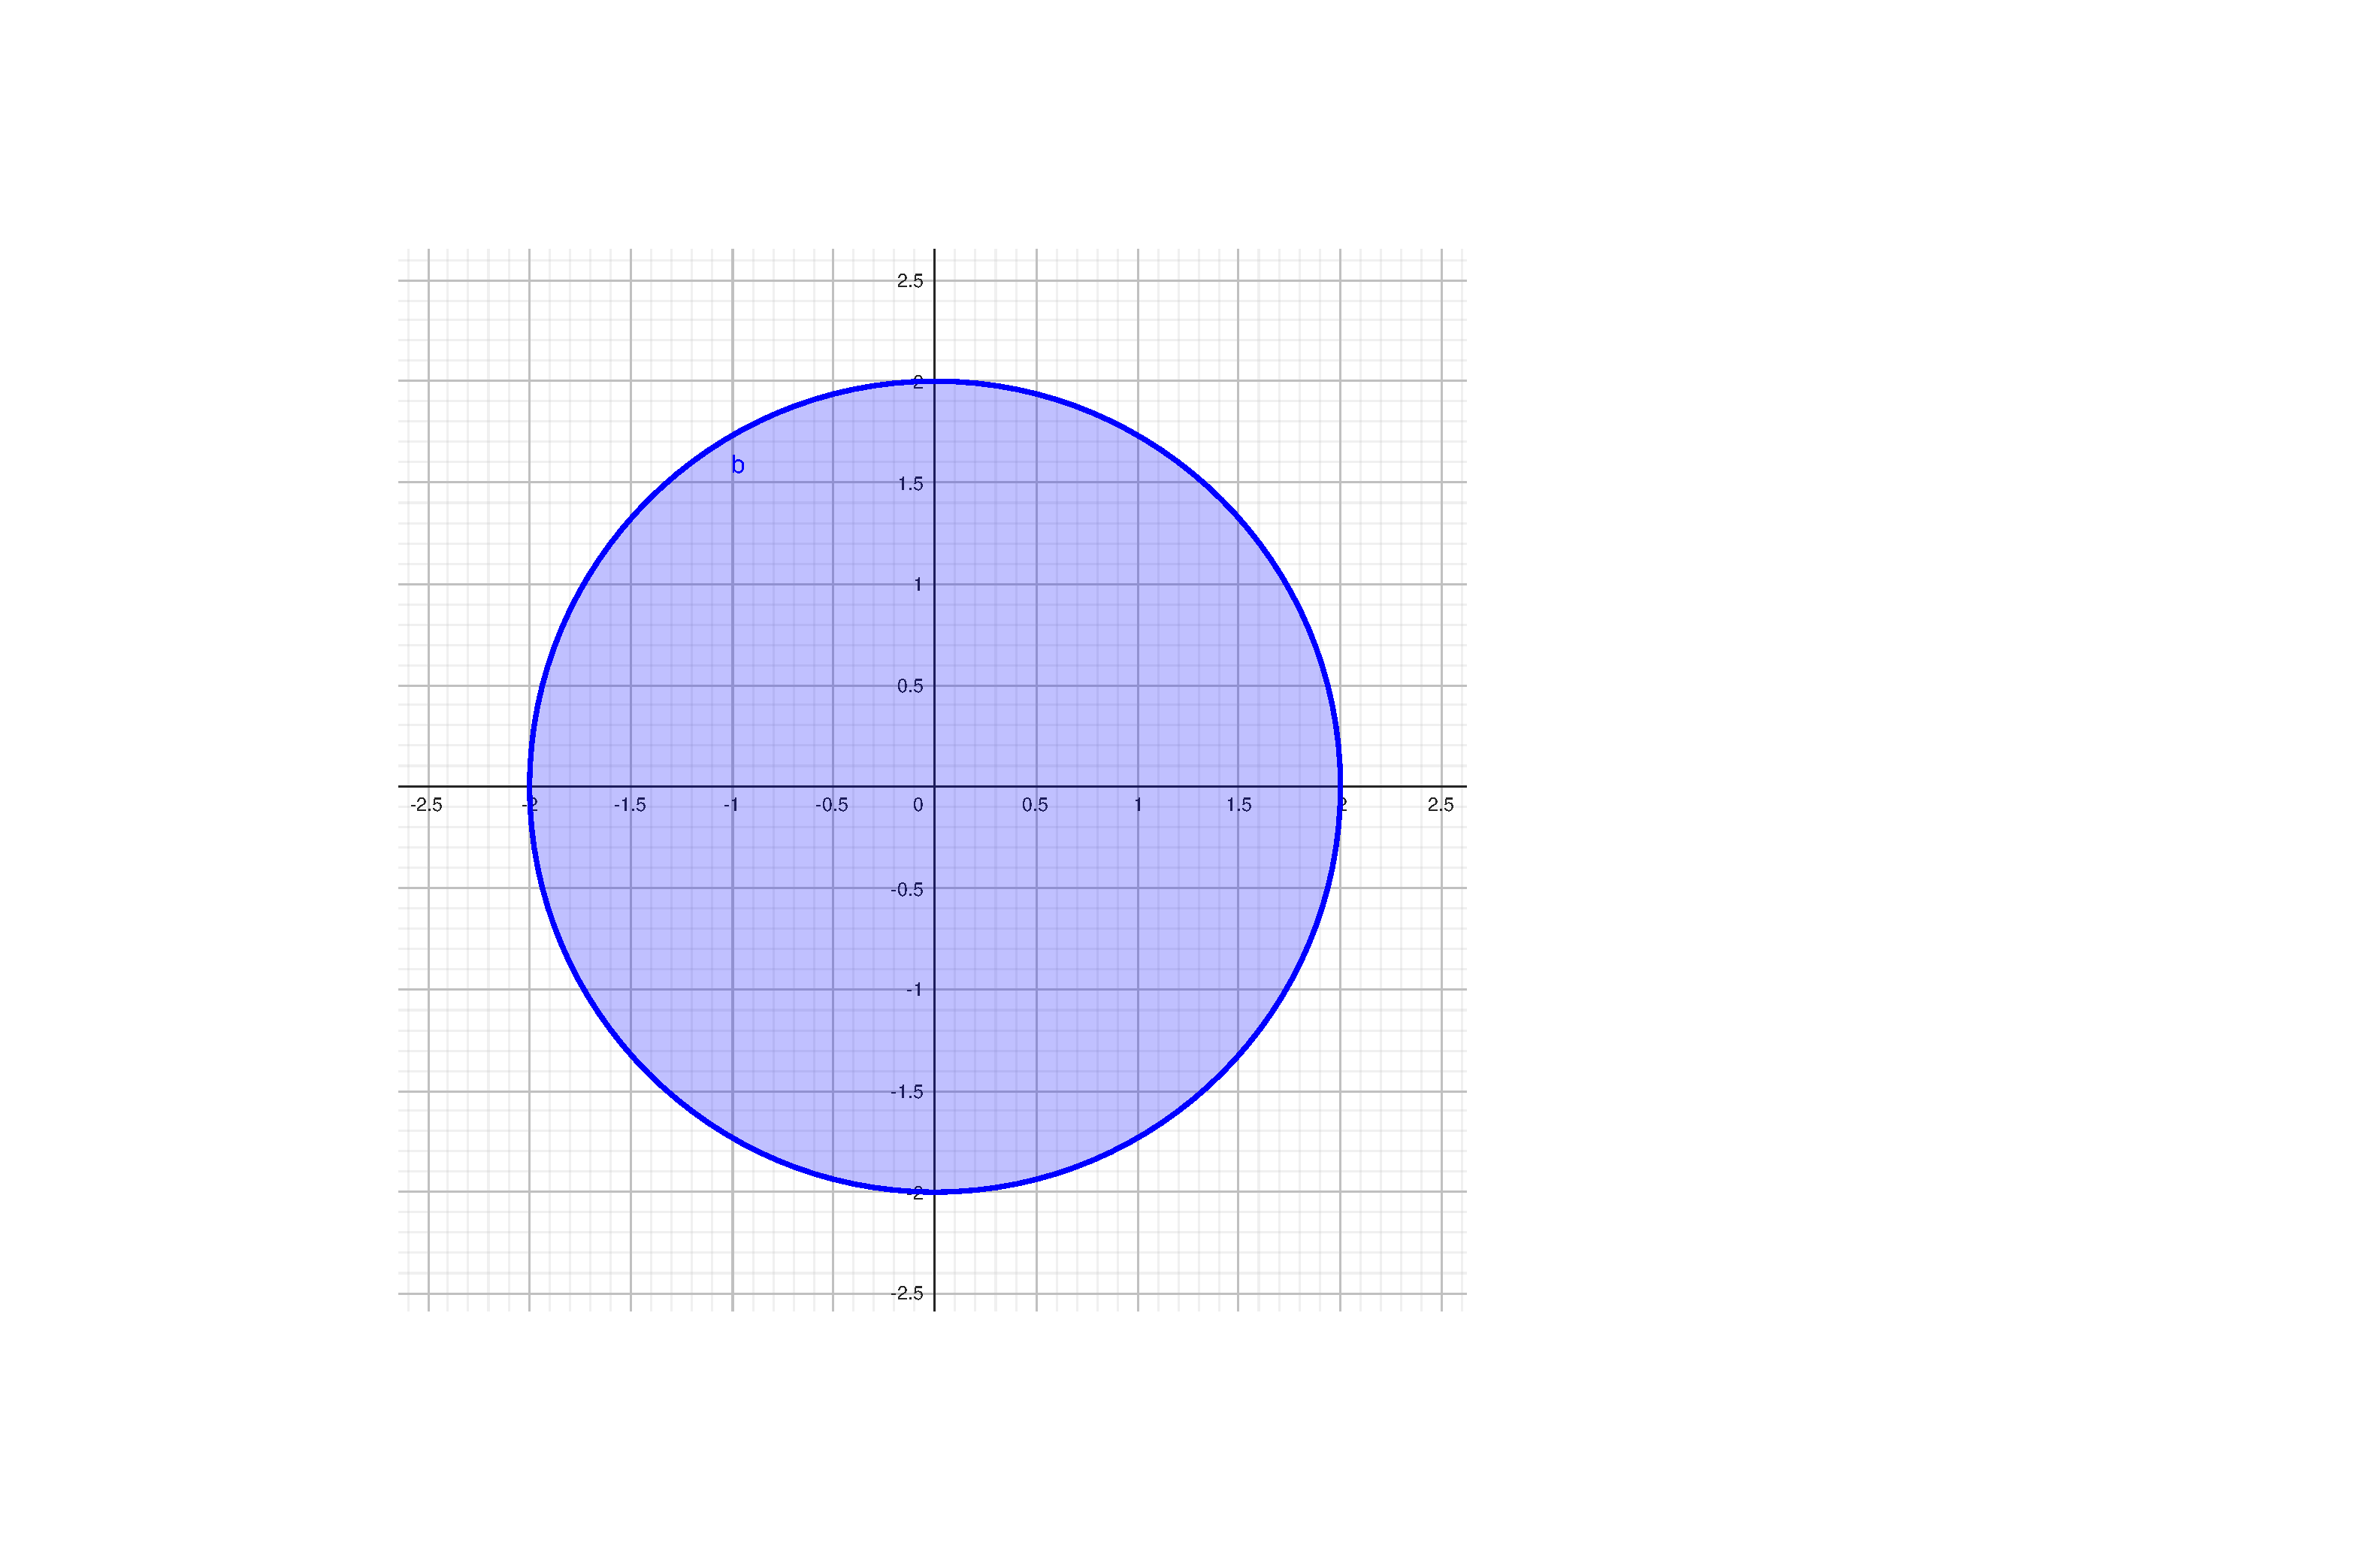
\includegraphics[width=\textwidth]{img/grafico-ex6-1.pdf}
			\caption*{1. Grafico di $x^{2} + y^{2} - 4 \le 0$}
		\end{figure}

		\item Si prosegue considerando la banale retta $x+y \ge 0$ che taglia il grafico a metà.
		\begin{figure}[!htp]
			\centering
			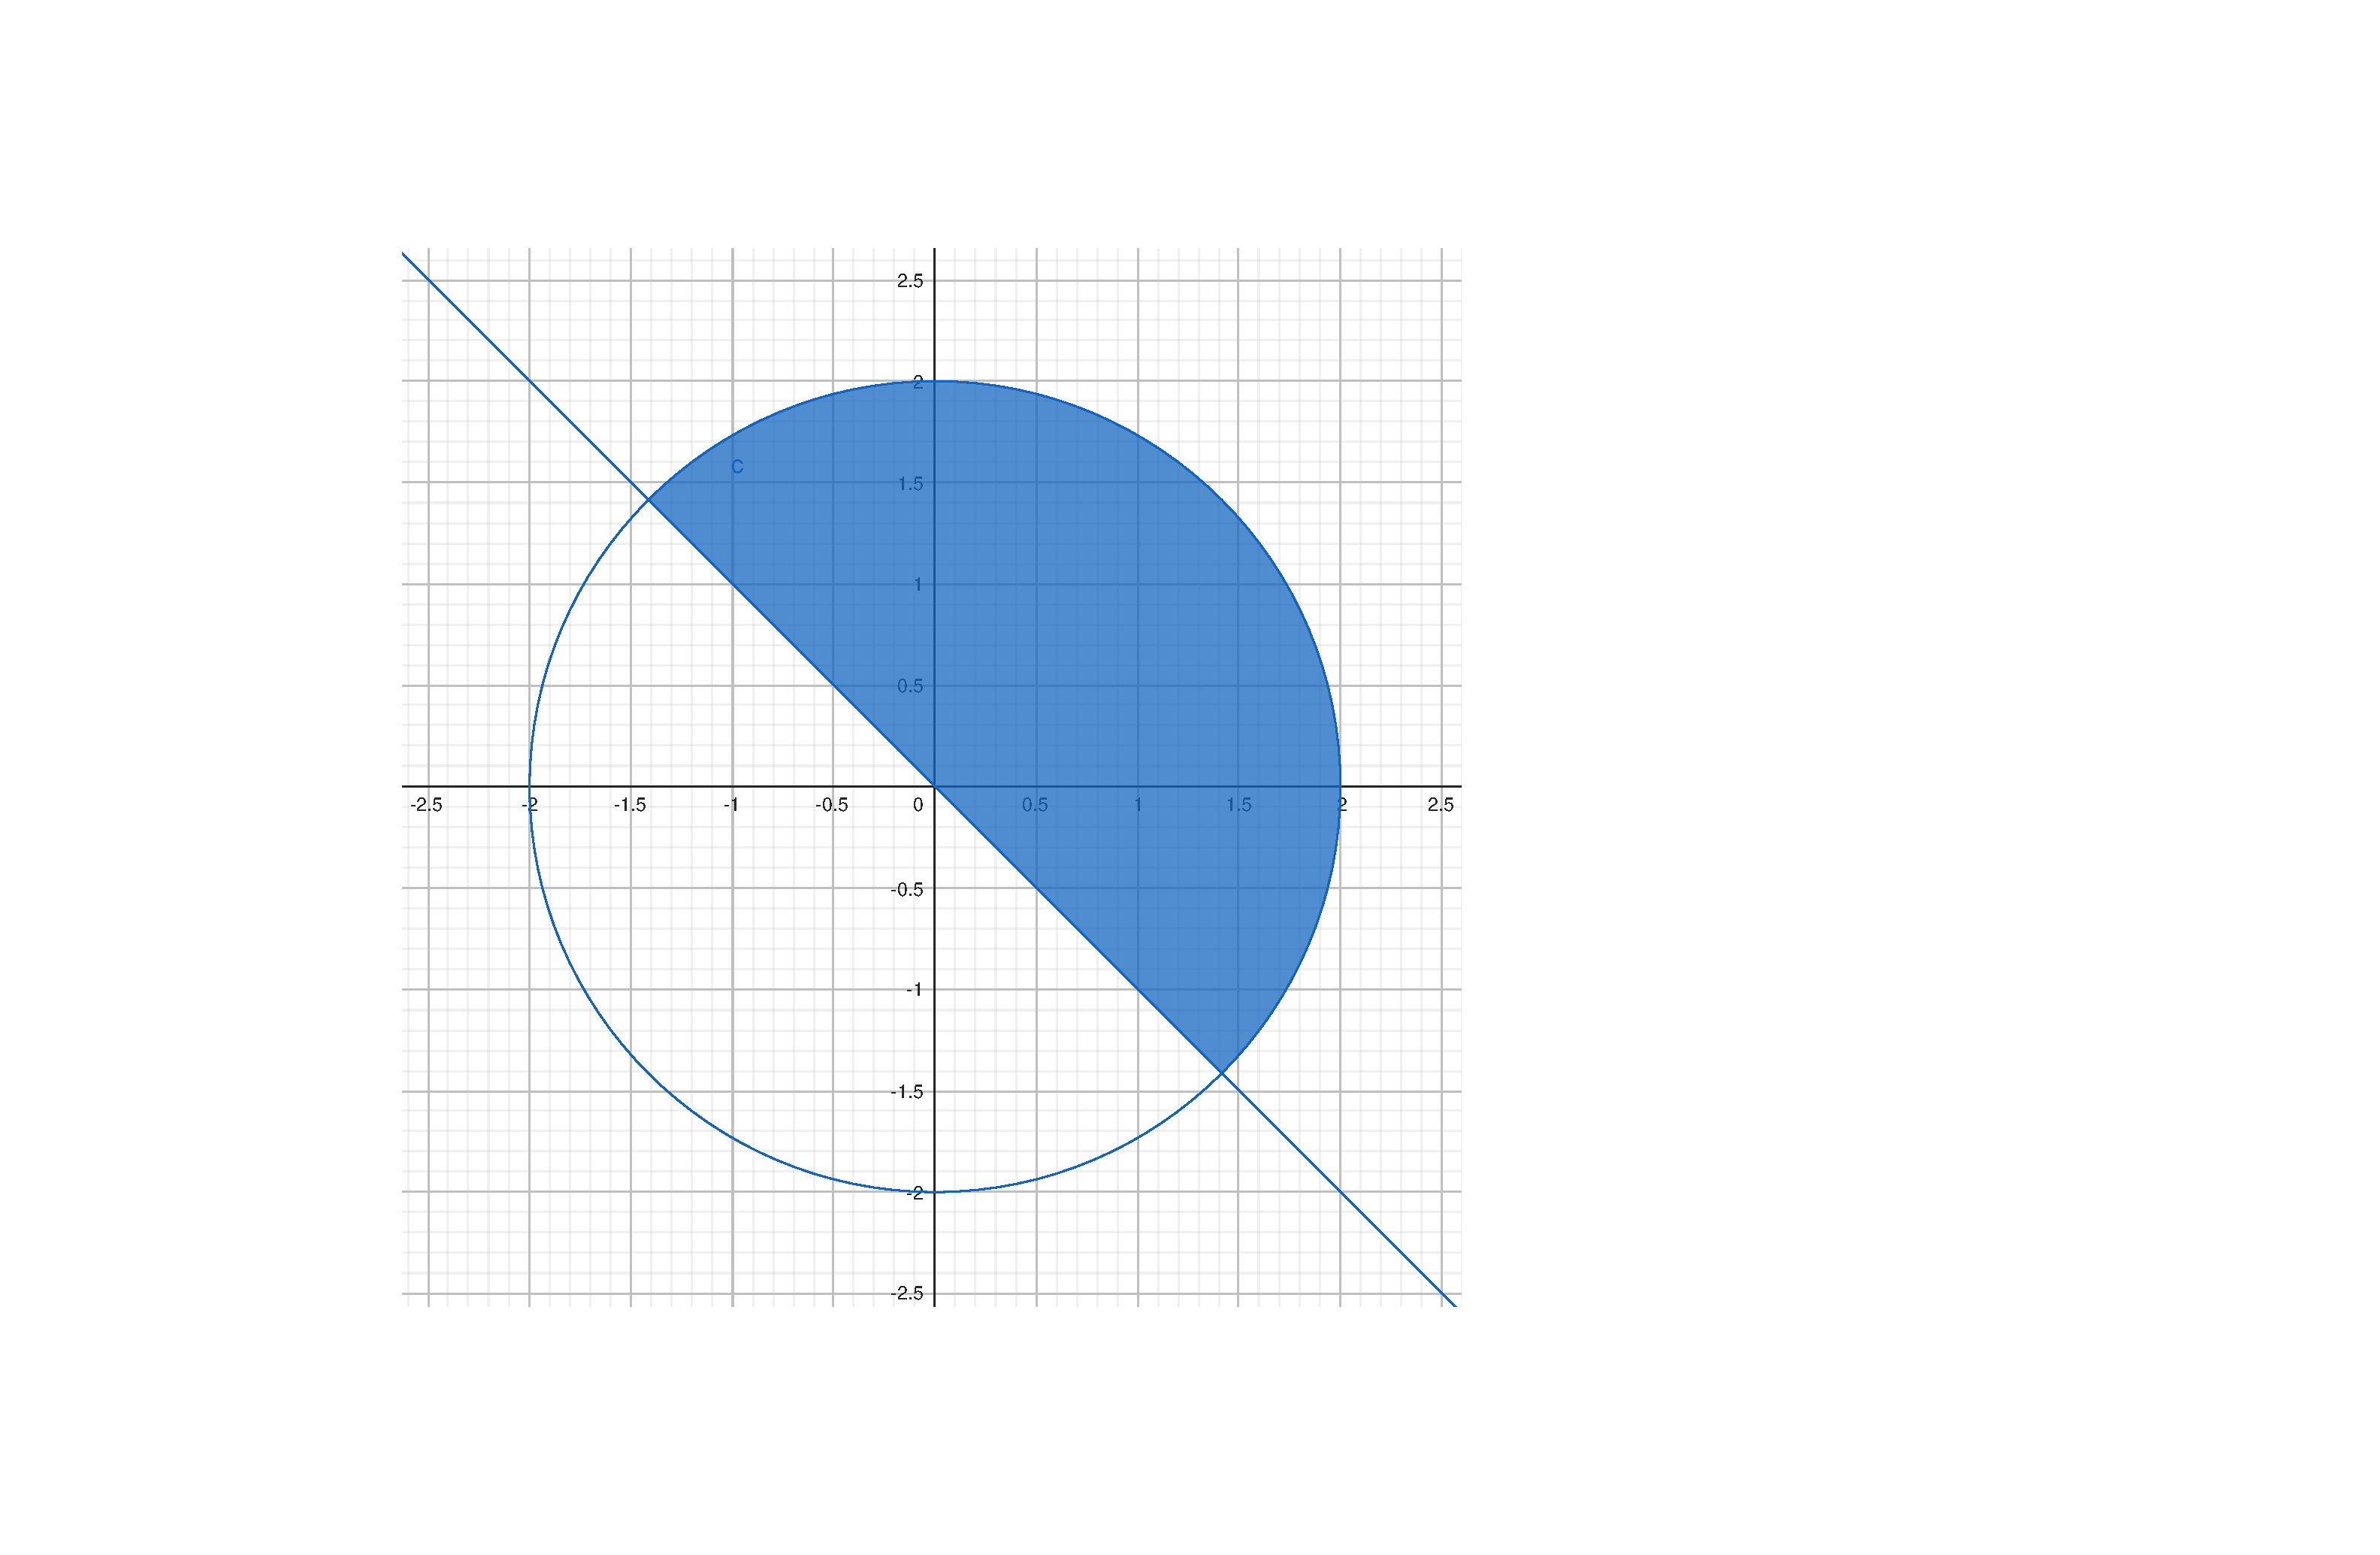
\includegraphics[width=\textwidth]{img/grafico-ex6-2.pdf}
			\caption*{2. Grafico di $x^{2} + y^{2} - 4 \le 0 \: \land \: x+y \ge 0$}
		\end{figure}

		\item Infine, si conclude considerando le due banalissime disuguaglianze $x \le 0$ e $y \ge 0$. Banali poiché con la condizione della $x$ si prendono solo i valori negativi e zero; invece, con la condizione della $y$ si prendono solo i valori positivi e zero.
		\begin{figure}[!htp]
			\centering
			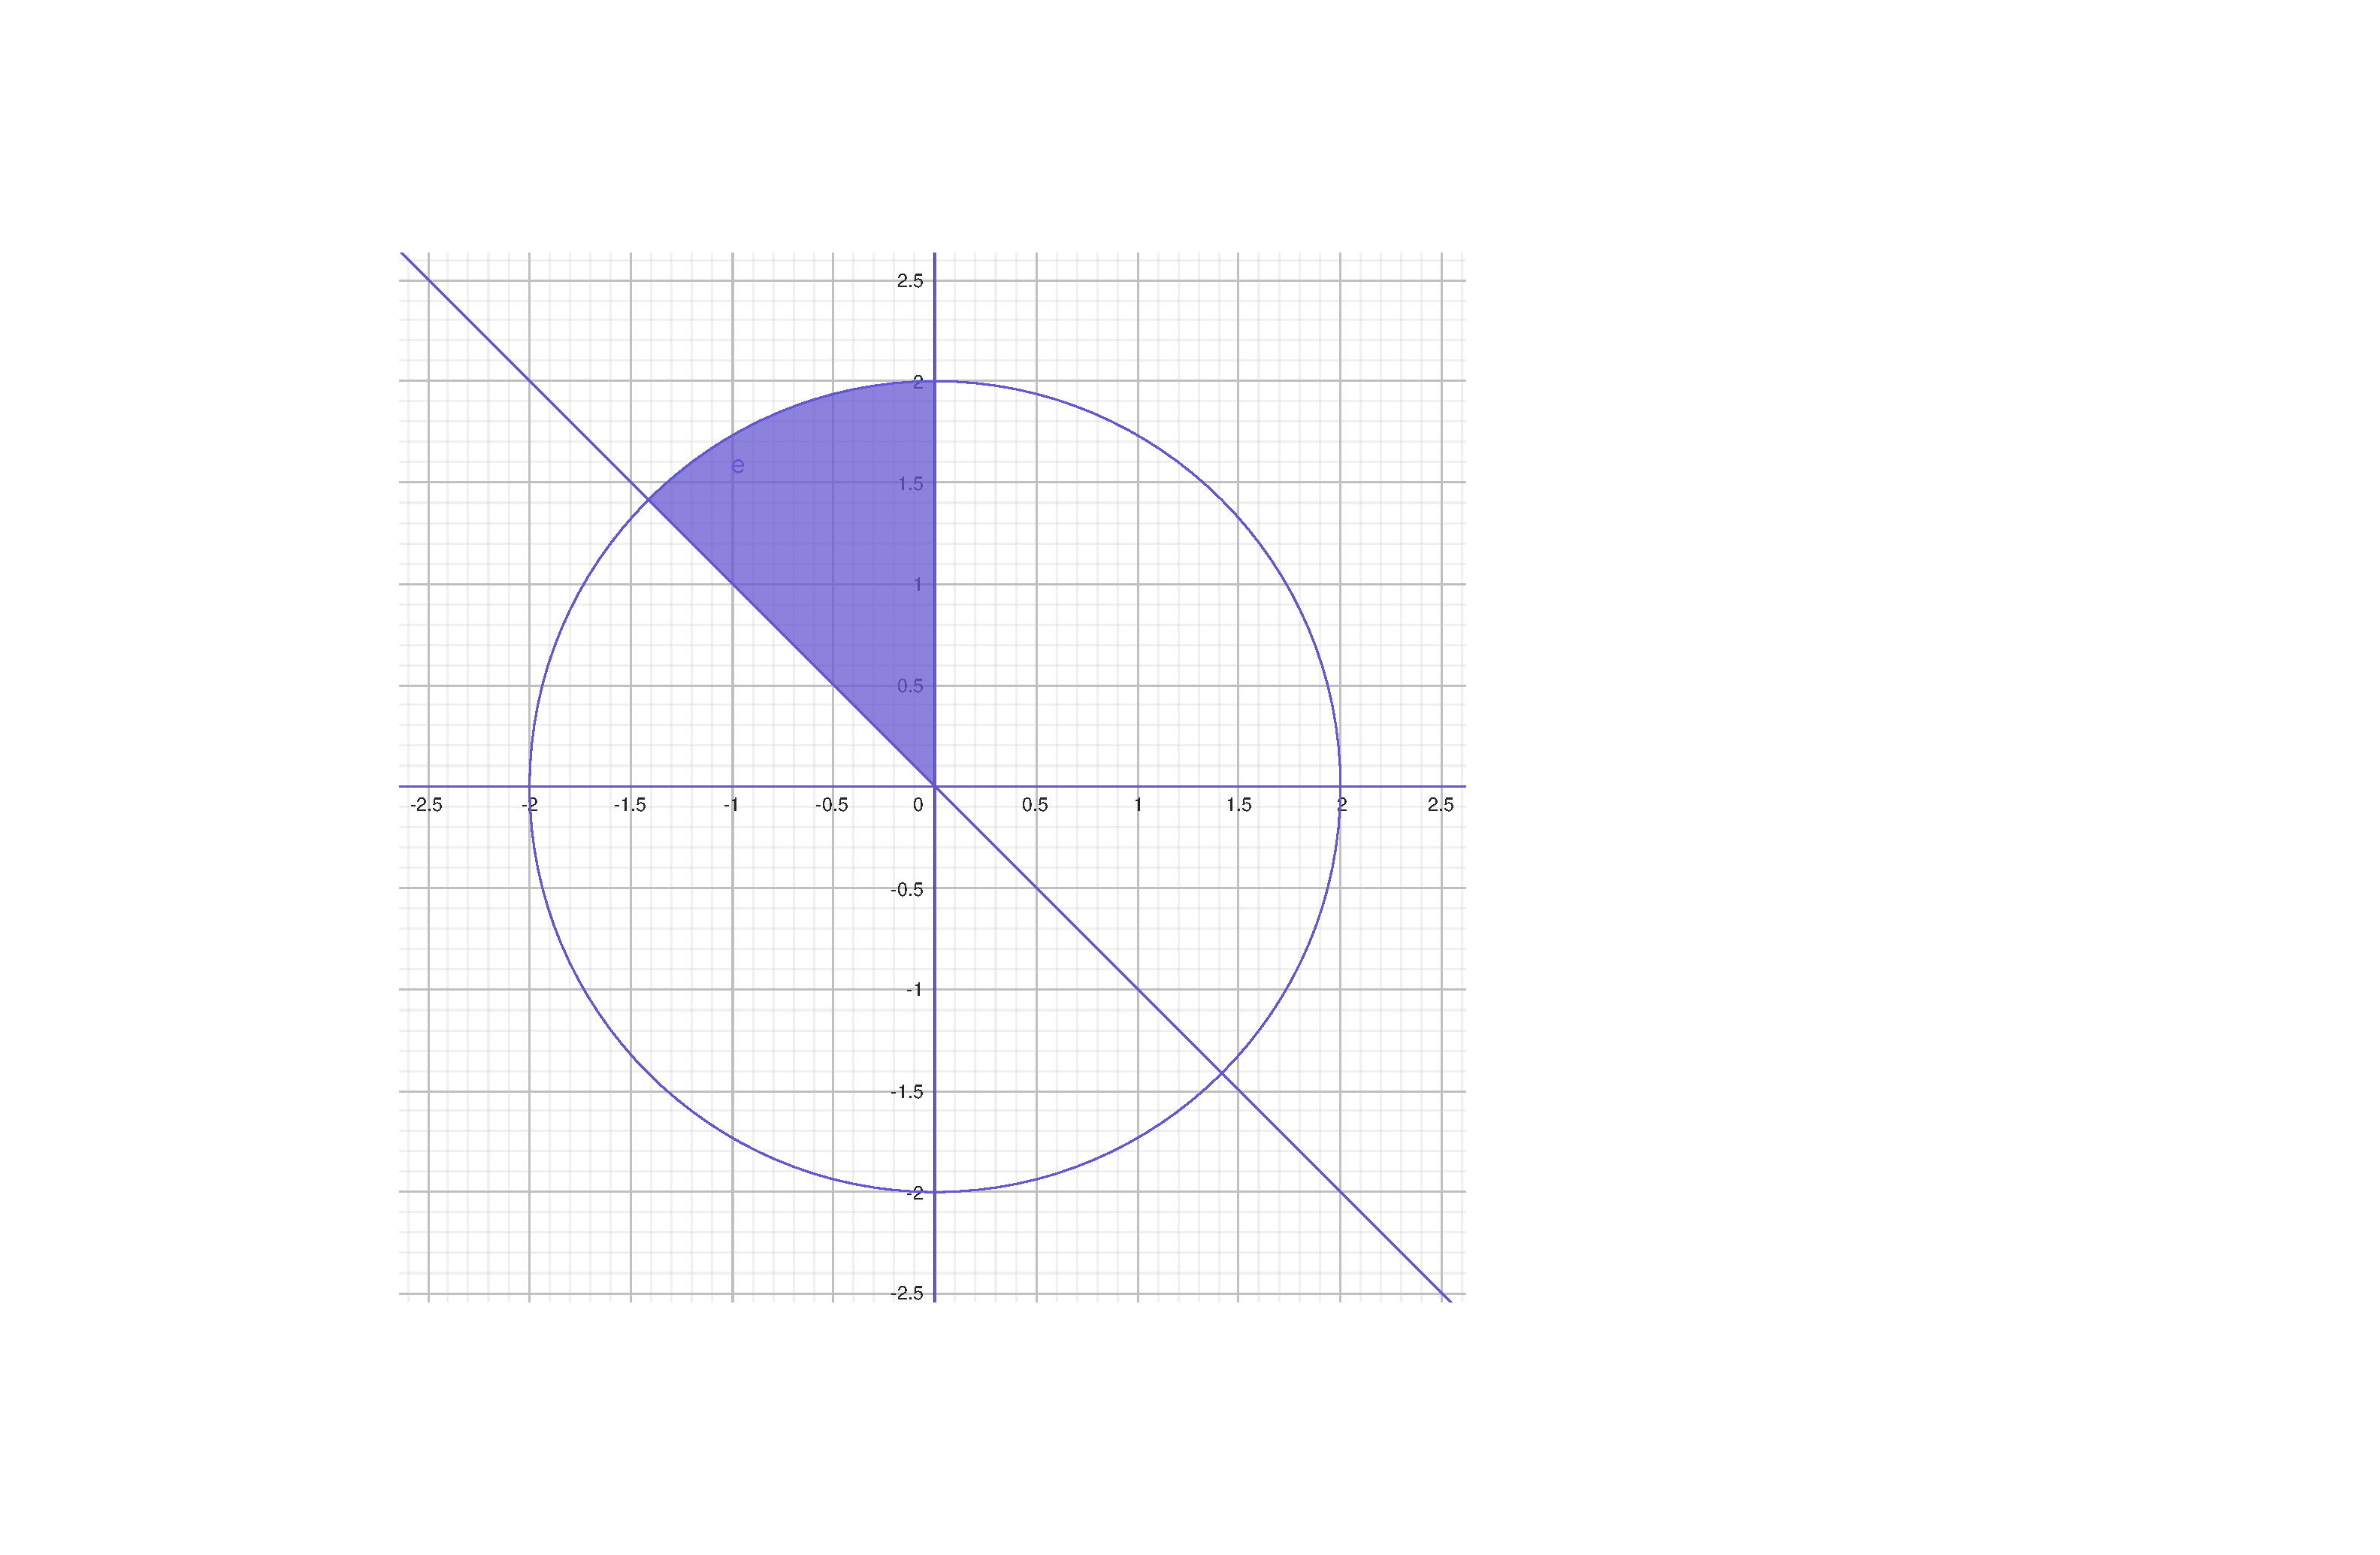
\includegraphics[width=\textwidth]{img/grafico-ex6-3.pdf}
			\caption*{3. Grafico di $x^{2} + y^{2} - 4 \le 0 \: \land \: x+y \ge 0 \: \land \: x \le 0 \: \land \: y \ge 0$}
			\label{fig: grafico ex6-3}
		\end{figure}
	\end{enumerate}
	Per capire il tipo di grafico rappresentato dalla figura, basta utilizzare il classico metodo della tabella $x$ e $y$. Quindi, si assegna un valore ad una delle due variabili e si esplicita l'altra incognita.\newpage

	\noindent
	Il \textbf{secondo passo} è ragionare sulla strategia da adottare. Una delle parti più complesse dell'esercizio è capire gli estremi di integrazione, ovvero i valori che dovranno andare agli estremi dell'integrale per calcolarlo. Le considerazioni da fare sono, per esempio: l'integrale presenta una forma $x^{2}+y^{2}$? Nel dominio $D$ vi è qualche circonferenza?
	
	Queste sono le classiche domande da porsi per capire se l'integrale è risolvibile tramite \textbf{coordinate polari}. Il metodo delle coordinate polari prevede la sostituzione dei termini così da avere un'integrazione più semplice e degli estremi facilmente riconoscibili.\newline

	\noindent
	Dopo aver deciso quale strategia adottare, il \textbf{terzo passo} è modificare il dominio portandolo nel sistema delle coordinate polari. Si ricorda che:
	\begin{equation*}
		\begin{cases}
			x = \rho\cos\left(\theta\right) \\
			y = \rho\sin\left(\theta\right)
		\end{cases}
	\end{equation*}
	Quindi, guardando la figura del dominio finale (pagina~\pageref{fig: grafico ex6-3}), si stabilisce nel seguente modo il nuovo dominio. L'angolo $\theta$ determina l'ampiezza dell'angolo, quindi, immaginando un osservatore posizionato sull'origine, cercando di guardare a destra e a sinistra quali sono i suoi limiti? Sono:
	\begin{itemize}
		\item L'asse delle $y$;
		\item Metà tra l'asse delle $x$ e delle $y$ (retta obliqua).
	\end{itemize}
	In un sistema trigonometrico, partendo dal punto $\left(x=2,y=0\right)$, quanti gradi si compie per arrivare al primo limite dell'osservatore sull'asse delle $y$ $\left(x=0, y=2\right)$? Esattamente $90$°. Invece, cercando di arrivare all'altro limite? Si compiono $90$° e metà di $90$, ovvero $45$°, per un totale di $90+45=135$°. Quindi, l'angolo $\theta$ è limitato tra:
	\begin{equation*}
		90\degree \le \theta \le 135\degree
	\end{equation*}
	Si convertono le misure da gradi a radianti:
	\begin{equation*}
		\begin{array}{rcl}
			1\degree &=& \dfrac{\pi}{180} \\ [1em]
			90\degree &=& 90 \cdot \dfrac{\pi}{180} = \dfrac{\pi}{2}	\\ [1em]
			135\degree &=& 135 \cdot \dfrac{\pi}{180} = \dfrac{3\pi}{4}
		\end{array}
	\end{equation*}
	E si riscrive la disuguaglianza:
	\begin{equation*}
		\dfrac{\pi}{2} \le \theta \le \dfrac{3\pi}{4}
	\end{equation*}
	Infine, manca $\rho$ da stabilire. Dato che con $\theta$ si ragiona sull'ampiezza, con $\rho$ si ragiona sulla lunghezza. Il dominio $D$ è limitato e chiuso, infatti, come si può vedere dalla figura, la massima distanza che può arrivare la vista dell'osservatore è il raggio, cioè $2$. Inoltre, l'osservatore è posizionato sull'origine, quindi il valore minimo sarà $0$:
	\begin{equation*}
		0 \le \rho \le 2
	\end{equation*}
	Quindi, il nuovo dominio diventa:
	\begin{equation*}
		D'=\left\{\left(x,y\right) \in \mathbb{R}^{2} \: : \: \dfrac{\pi}{2} \le \theta \le \dfrac{3\pi}{4}, 0 \le \rho \le 2\right\}
	\end{equation*}\newpage

	\noindent
	Si noti adesso come l'aria di integrazione sia diventata molto più banale:
	\begin{figure}[!htp]
		\centering
		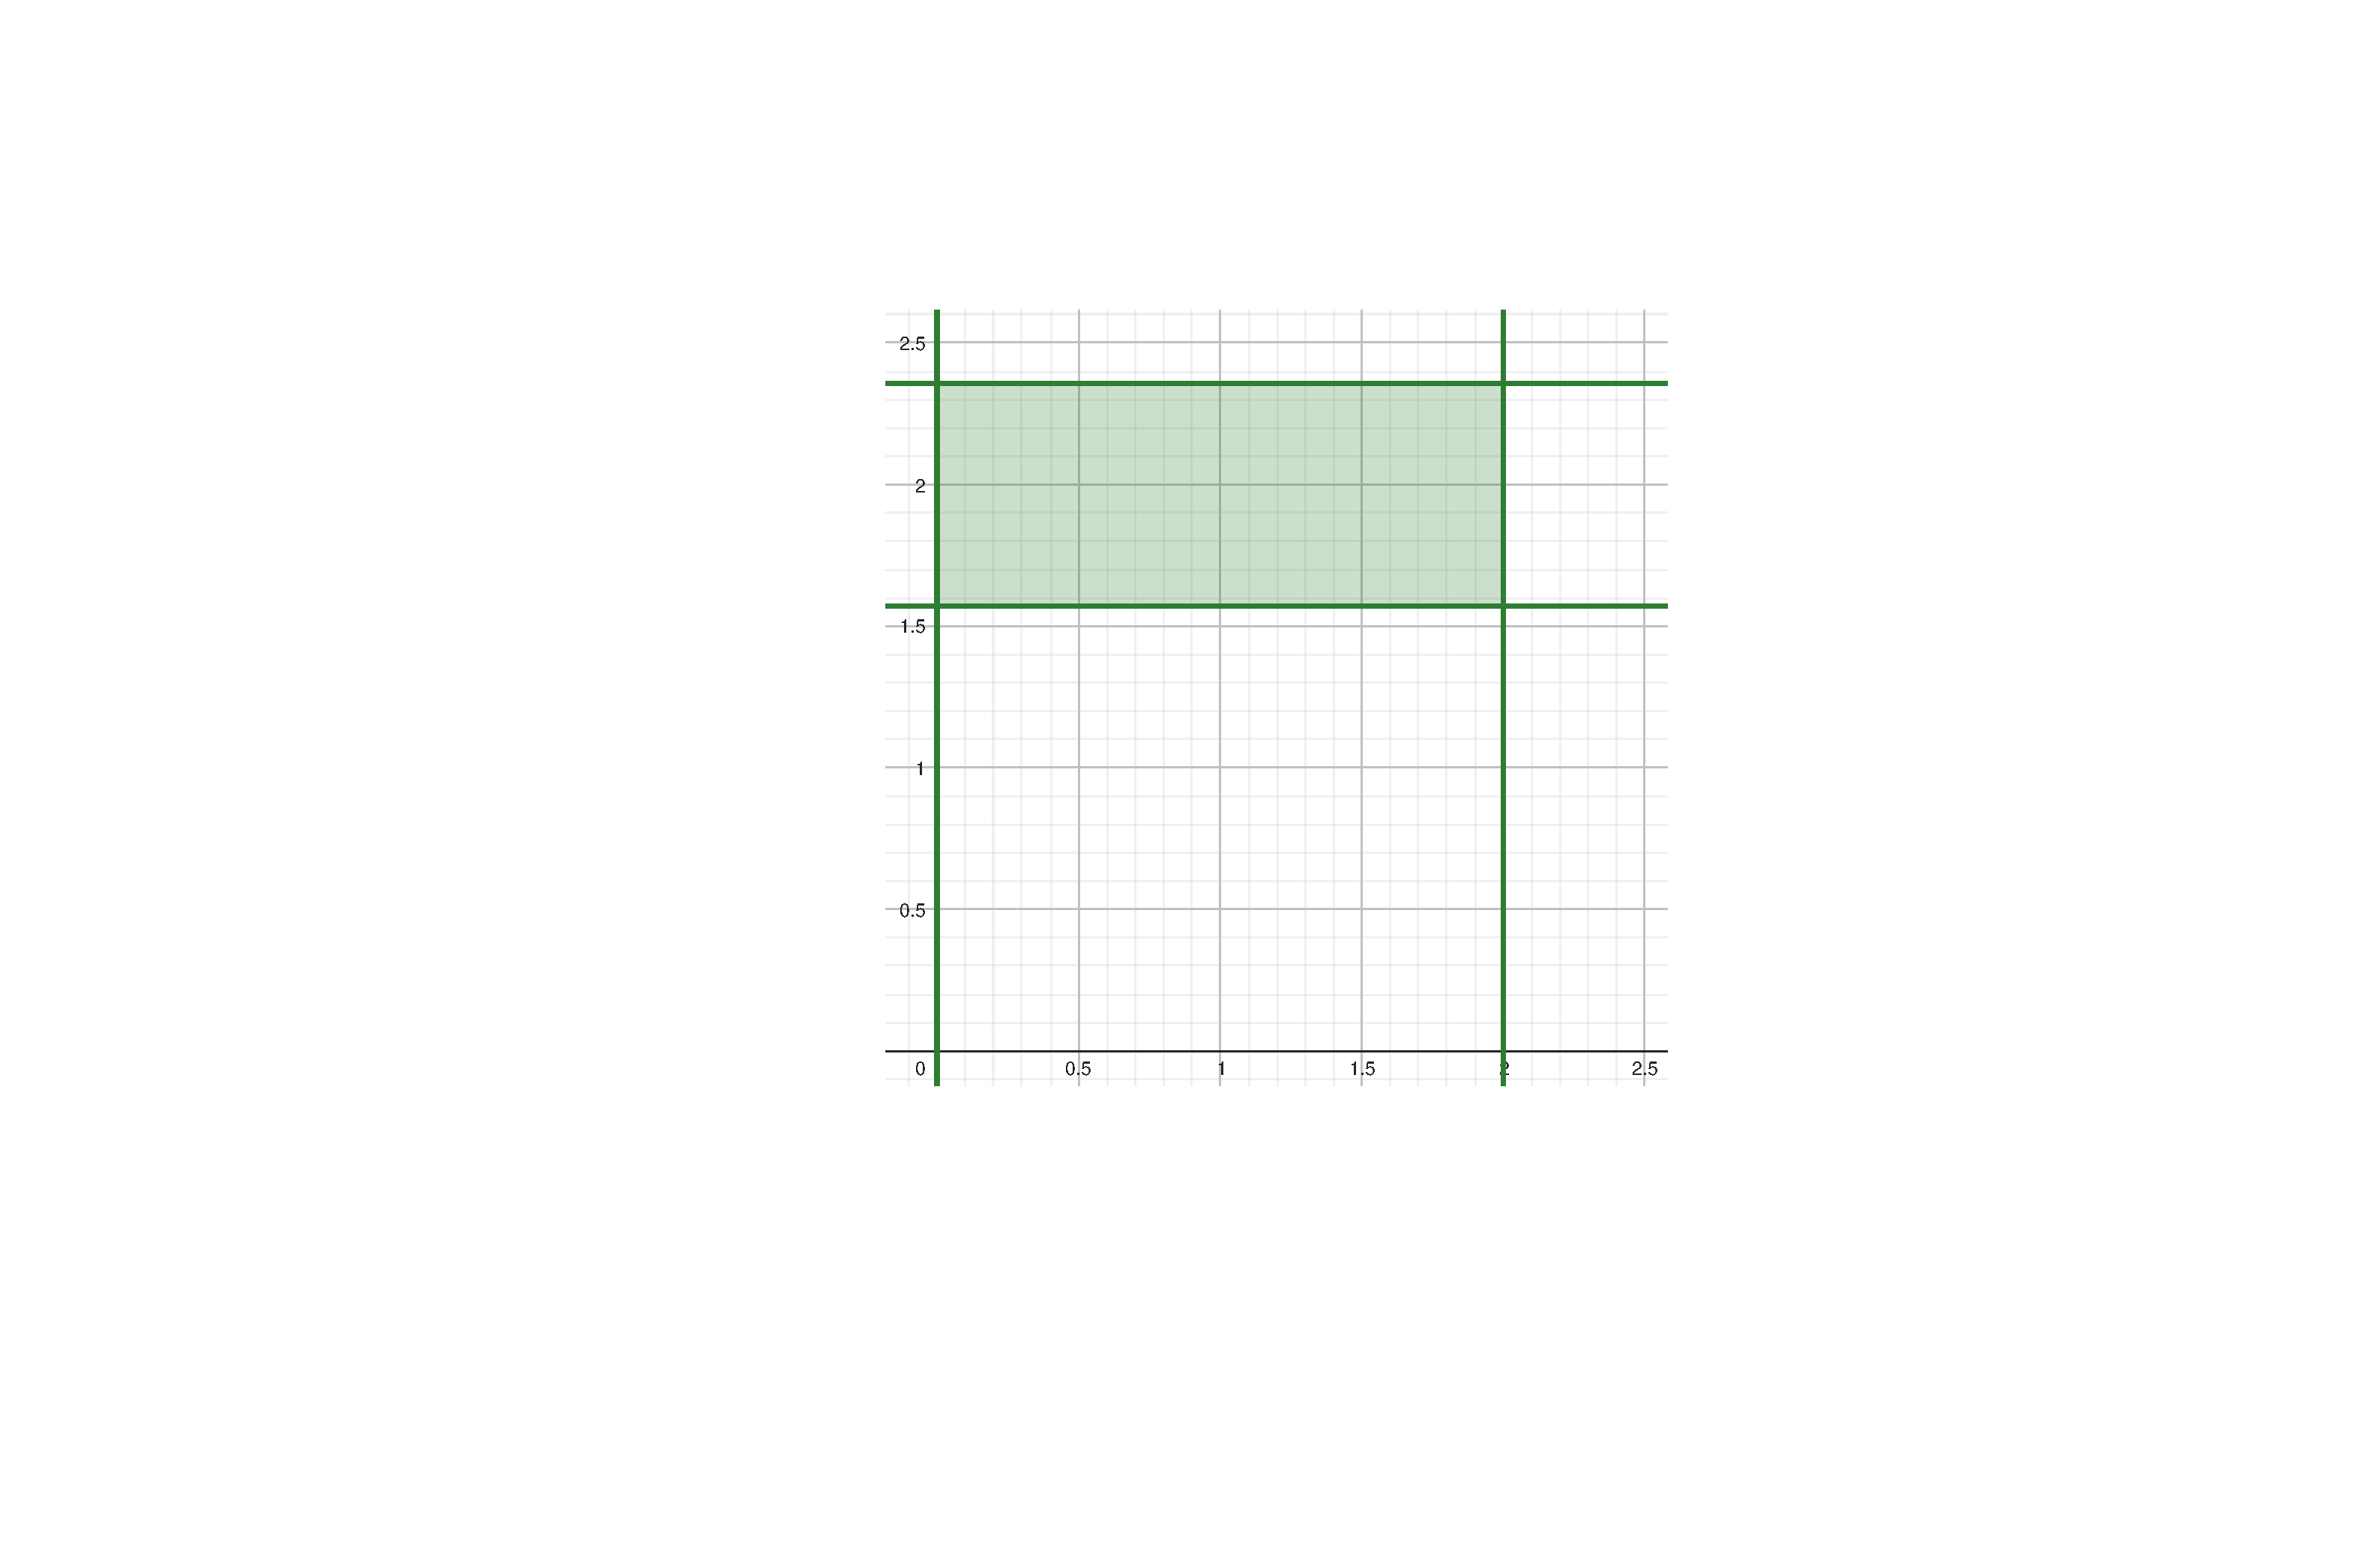
\includegraphics[width=.7\textwidth]{img/grafico-ex6-4.pdf}
		\caption*{4. Dominio $D'$}
	\end{figure}

	\noindent
	Il \textbf{quarto passo} è risolvere l'integrale vero e proprio. Si scrivono gli estremi di integrazione e si sostituiscono a tutte le $x=\rho\cos\left(\theta\right)$ e a tutte le $y=\rho\sin\left(\theta\right)$ (come detto nella pagina precedente):
	\begin{equation*}
		\displaystyle\int_{\frac{\pi}{2}}^{\frac{3\pi}{4}} \int_{0}^{2} \dfrac{1}{\left(1+ \rho^{2}\cos^{2}\left(\theta\right) + \rho^{2}\sin^{2}\left(\theta\right)\right)^{3}} \cdot \rho \: \mathrm{d}\rho\mathrm{d}\theta
	\end{equation*}
	L'unità $\rho$ moltiplica l'integrale per una questione teorica (matrice Jacobiana). Si conclude quindi l'esercizio con la risoluzione dell'integrale.\newpage 
	
	\noindent
	Si risolve l'integrale:
	\begin{equation*}
		\begin{array}{cl}
			=& \displaystyle\int_{\frac{\pi}{2}}^{\frac{3\pi}{4}} \int_{0}^{2} \dfrac{1}{(1+ \rho^{2} \underbrace{\left(\cos^{2}\left(\theta\right) + \sin^{2}\left(\theta\right)\right)}_{=1})^{3}} \cdot \rho \: \mathrm{d}\rho\mathrm{d}\theta \\[1em]
			%
			=& \displaystyle\int_{\frac{\pi}{2}}^{\frac{3\pi}{4}} \int_{0}^{2} \dfrac{\rho}{\left(1 + \rho^{2}\right)^{3}} \: \mathrm{d}\rho\mathrm{d}\theta \\ [1.5em]
			%
			\rightarrow& \text{si risolve per sostituzione: }\mathrm{d}\rho = \dfrac{1}{t'} \cdot \mathrm{d}t; \hspace{1em} t = 1+\rho^{2}; \hspace{1em} t'=2\rho \\ [.7em]
			%
			=& \displaystyle\int_{\frac{\pi}{2}}^{\frac{3\pi}{4}} \int_{0}^{2} \dfrac{\rho}{\left(t\right)^{3}} \cdot \dfrac{1}{2\rho} \: \mathrm{d}t\mathrm{d}\theta \\ [1.5em]
			%
			=& \displaystyle\int_{\frac{\pi}{2}}^{\frac{3\pi}{4}} \int_{0}^{2} \dfrac{1}{t^{3}} \cdot \dfrac{1}{2} \: \mathrm{d}t\mathrm{d}\theta \\ [1.5em]
			%
			=& \displaystyle\int_{\frac{\pi}{2}}^{\frac{3\pi}{4}} \left( \dfrac{1}{2} \cdot \int_{0}^{2} \dfrac{1}{t^{3}} \: \mathrm{d}t \right) \mathrm{d}\theta \\ [1.5em]
			%
			\rightarrow& \text{ricordando che: } \displaystyle\int\dfrac{1}{x^{n}} = -\dfrac{1}{\left(n-1\right) \cdot x^{n-1}}, n \ne 1 \\ [.7em]
			%
			=& \displaystyle\int_{\frac{\pi}{2}}^{\frac{3\pi}{4}} \left[\dfrac{1}{2} \cdot - \dfrac{1}{2t^2}\right]_{0}^{2} \mathrm{d}\theta \\ [1.5em]
			%
			\rightarrow& \text{si rimuove la }t \\ [.7em]
			%
			=& \displaystyle\int_{\frac{\pi}{2}}^{\frac{3\pi}{4}} \left[\dfrac{1}{2} \cdot - \dfrac{1}{2 \cdot \left(1 + 2\rho^{2} + \rho^{4}\right)}\right]_{0}^{2} \mathrm{d}\theta \\ [1.5em]
			%
			=& \displaystyle\int_{\frac{\pi}{2}}^{\frac{3\pi}{4}} \left[- \dfrac{1}{4+8\rho^{2}+4\rho^{4}}\right]_{0}^{2} \mathrm{d}\theta \\ [1.5em]
			%
			=& \displaystyle\int_{\frac{\pi}{2}}^{\frac{3\pi}{4}} \left(-\dfrac{1}{4 + 8 \cdot 2^{2} + 4 \cdot 2^{4}} - \left(-\dfrac{1}{4 + 8 \cdot 0^{2} + 4 \cdot 0^{4}}\right)\right) \: \mathrm{d}\theta \\ [1.5em]
			%
			=& \displaystyle\int_{\frac{\pi}{2}}^{\frac{3\pi}{4}} \left(-\dfrac{1}{100} + \dfrac{1}{4}\right) \: \mathrm{d}\theta \\ [1.5em]
			%
			=& \displaystyle\int_{\frac{\pi}{2}}^{\frac{3\pi}{4}} \dfrac{24}{100} \: \mathrm{d}\theta \\ [1.5em]
			%
			=& \displaystyle\int_{\frac{\pi}{2}}^{\frac{3\pi}{4}} \dfrac{6}{25} \: \mathrm{d}\theta \\ [1.5em]
			%
			=& \left[\dfrac{6}{25}\theta\right]_{\frac{\pi}{2}}^{\frac{3\pi}{4}} \\ [1.5em]
			%
			=& \dfrac{6}{25} \cdot \dfrac{3\pi}{4} - \dfrac{6}{25} \cdot \dfrac{\pi}{2} \\ [1.5em]
			%
			=& \dfrac{9\pi}{50} - \dfrac{3\pi}{25} = \dfrac{3\pi}{50}
		\end{array}
	\end{equation*}\newpage

	\subsubsection{$x$-semplice e $y$-semplice - Calcolo integrale doppio con insieme definito da punti}\label{par: x-semplice e y-semplice - calcolo integrale doppio}

	Questa tecnica, se trovata in un esame, è una delle più semplici. Questo paragrafo, oltre a introdurre tale tecnica, presenta anche il caso in cui l'esercizio dia solo dei punti e non un insieme definito. Si prenda in considerazione il tema d'esame del 07/02/2023: \textcolor{Green4}{\textbf{\emph{Calcolare:}}
	\begin{equation*}
		\underset{D}{\int\hspace{-.5em}\int} \left(y-2x\right) \: \mathrm{d}x \: \mathrm{d}y
	\end{equation*}
	\textbf{\emph{dove $D$ è la regione del piano limitata dal quadrilatero di vertici $\left(-1,0\right)$, $\left(0,0\right)$, $\left(-1,2\right)$, $\left(-2,2\right)$. Dare un'interpretazione geometrica o fisica del risultato ottenuto.}}}\newline

	\noindent
	Non viene dato un dominio, quindi il \textbf{primo passo} è marcare i punti dati sul piano cartesiano così da disegnare l'area interessata. I punti vengono collegati secondo le direttive dell'esercizio, in questo caso ci viene esplicitamente scritto che è un quadrilatero:
	\begin{figure}[!htp]
		\centering
		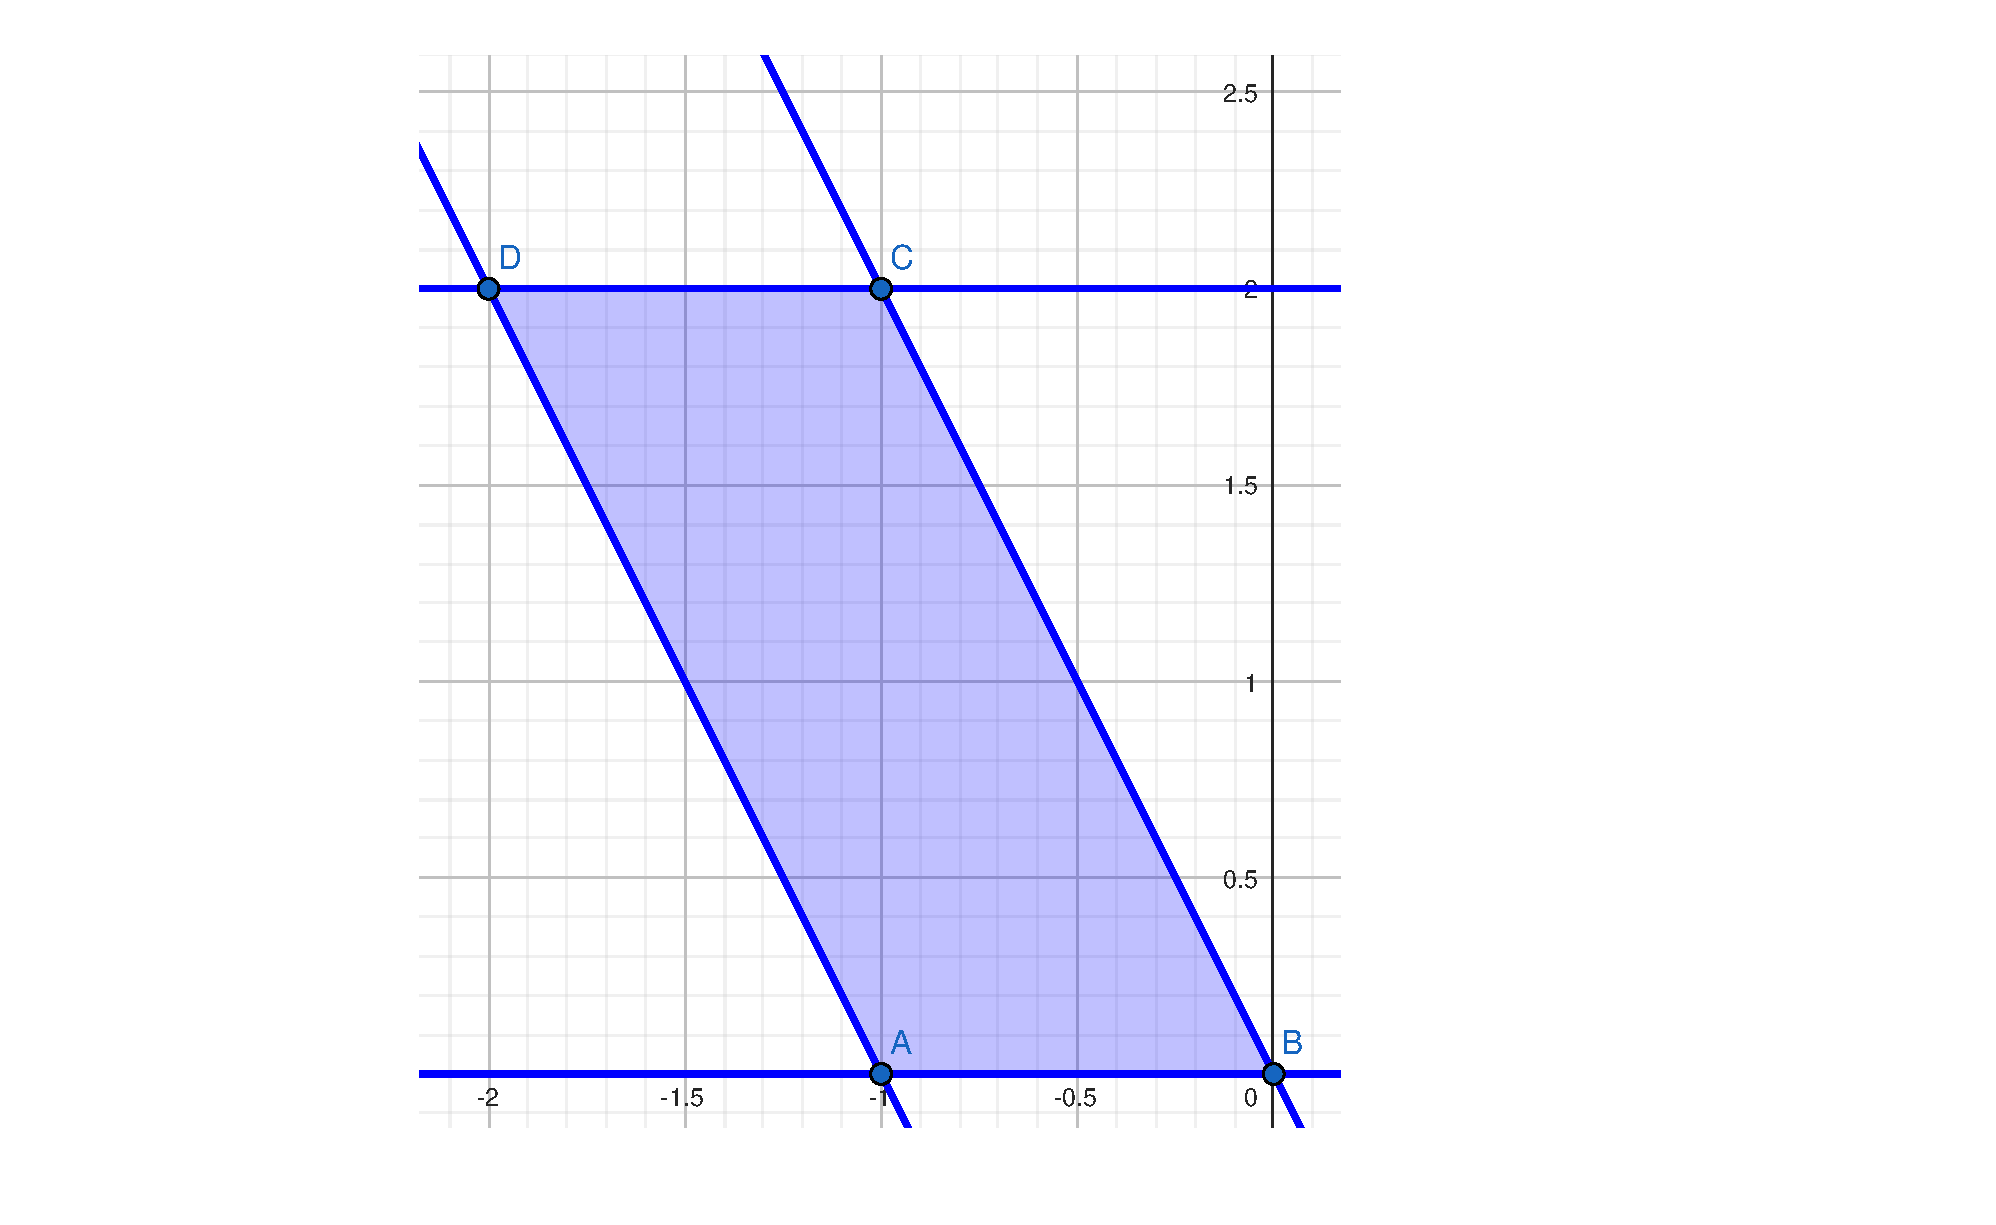
\includegraphics[width=.8\textwidth]{img/grafico-ex6-5.pdf}
		\caption*{Il dominio cercato.}
	\end{figure}\newpage

	\noindent
	Il \textbf{secondo passo} è riscrivere il dominio. Per farlo, si cerca prima di capire se si è intenzionati a integrare per $x$-semplice o $y$-semplice.
	\begin{mdframed}
		\textbf{\emph{Teoria generale dell'integrazione per $x$-semplice e $y$-semplice}}\newline

		\noindent
		L'integrazione per \underline{$x$-semplice} viene applicata quando il dominio è delimitato rispetto all'asse delle $x$ da due valori e rispetto all'asse delle $y$ da due funzioni:
		\begin{center}
			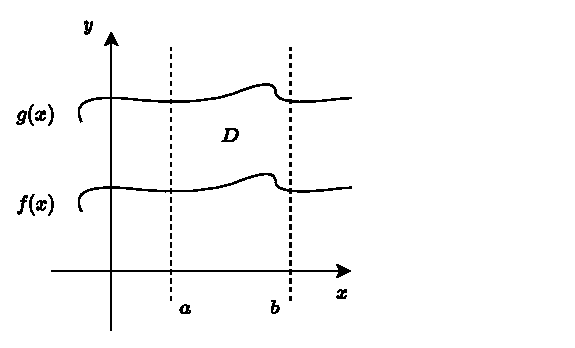
\includegraphics[width=.35\textwidth]{img/grafico-ex6-6.pdf}
		\end{center}
		Così facendo, il dominio e l'integrale saranno:
		\begin{gather*}
			D = \left\{\left(x,y\right) \in \mathbb{R}^{2} \: : \: a \le x \le b, \: f\left(x\right) \le y \le g\left(x\right)\right\} \\
			\int_{a}^{b} \left(\int_{f\left(x\right)}^{g\left(x\right)} \varphi\left(x,y\right) \: \mathrm{d}y\right) \: \mathrm{d}x
		\end{gather*}
		%
		Al contrario, con l'integrazione per \underline{$y$-semplice}, si applica quando il dominio è limitato rispetto ad $x$ da dei valori e rispetto $y$ da delle funzioni:
		\begin{center}
			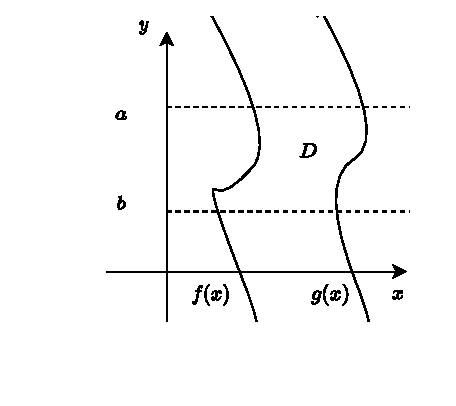
\includegraphics[width=.35\textwidth]{img/grafico-ex6-7.pdf}
		\end{center}
		Così facendo, il dominio sarà del tipo:
		\begin{gather*}
			D = \left\{\left(x,y\right) \in \mathbb{R}^{2} \: : \: a \le y \le b, \: f\left(y\right) \le x \le g\left(y\right)\right\} \\
			\int_{a}^{b} \left(\int_{f\left(x\right)}^{g\left(x\right)} \varphi\left(x,y\right) \: \mathrm{d}x\right) \: \mathrm{d}y
		\end{gather*}
		\textbf{\underline{N.B.}} nel dominio le lettere $a,b$ devono essere valori numerici, mentre le funzioni non devono dipendere dalla stessa variabile! Quindi, non può esistere (e.g. nella $y$-semplice) il caso in cui $x$ sia compreso tra due funzioni di $x$: $\cancel{f\left(x\right) \le x \le g\left(x\right)}$ \textcolor{Red3}{\textbf{ NO! \ding{55}}}\newline
		Tuttavia, possono essere valori numerici gli estremi: $0 \le x \le g\left(y\right)$ \textcolor{Green4}{\textbf{ SÌ \ding{51}}}
	\end{mdframed}\newpage

	\noindent
	Come si vede dal grafico, il dominio è limitato da due rette rispetto a $y$ (parallele a $x$), ovvero $y = 0$ e $y = 2$. Ne consegue, che conviene applicare l'integrazione per $y$-semplice.\newline

	\noindent
	Per trovare il dominio, è necessario calcolare l'equazione delle due rette. Per farlo, si utilizza la formula elementare per calcolare l'equazione di una retta passante per due punti:
	\begin{gather*}
		\dfrac{x-x_{1}}{x_{2} - x_{1}} = \dfrac{y-y_{1}}{y_{2} - y_{1}} \\
		\\
		\begin{array}{rcl}
			\left(0,0\right) \rightarrow \left(-1,2\right) &\longrightarrow& \dfrac{x-0}{-1 - 0} = \dfrac{y-0}{2-0} \\
			\\
			&\longrightarrow& x = -\dfrac{1}{2}y \\
			\\
			\left(-1,0\right) \rightarrow \left(-2,2\right) &\longrightarrow& \dfrac{x+1}{-2-\left(-1\right)} = \dfrac{y-0}{2 - 0} \\
			\\
			&\longrightarrow& x = - \dfrac{1}{2}y-1 \\
		\end{array}
	\end{gather*}
	Quindi, il dominio è:
	\begin{equation*}
		D = \left\{\left(x,y\right) \in \mathbb{R}^{2} \: : \: \left(0 \le y \le 2\right), \: \left(-\dfrac{1}{2}y-1 \le x \le -\dfrac{1}{2}y\right)\right\}
	\end{equation*}
	Il \textbf{terzo passo} è risolvere l'integrale con gli estremi di integrazione trovati e concludere l'esercizio, quindi:
	\begin{equation*}
		\begin{array}{ll}
			=& \displaystyle\int_{0}^{2} \int_{-\frac{1}{2}y-1}^{-\frac{1}{2}y} \left(y-2x\right) \: \mathrm{d}x \: \mathrm{d}y \\ [1.5em]
			%
			=& \displaystyle\int_{0}^{2} \left[xy - x^{2}\right]_{-\frac{1}{2}y-1}^{-\frac{1}{2}y} \: \mathrm{d}y \\ [1.5em]
			%
			=& \displaystyle\int_{0}^{2} \left[ \left(-\dfrac{1}{2}y\right)y - \left(-\dfrac{1}{2}y\right)^{2} \right] - \left[ \left(-\dfrac{1}{2}y-1\right)y - \left(-\dfrac{1}{2}y-1\right)^{2} \right] \: \mathrm{d}y \\[1.5em]
			%
			=& \displaystyle\int_{0}^{2} -\dfrac{1}{2}y^{2} - \dfrac{1}{4}y^{2} + \dfrac{1}{2}y^{2} + y + \dfrac{1}{4}y^{2} + y + 1 \: \mathrm{d}y \\ [1.5em]
			%
			=& \displaystyle\int_{0}^{2} 2y + 1 \: \mathrm{d}y \\ [1.5em]
			%
			=& \left[y^{2} + y\right]_{0}^{2} \\ [1em]
			%
			=& 2^{2} + 2 - 0^{2} + 0 \\ [1em]
			%
			=& 6
		\end{array}
	\end{equation*}\newpage

	\subsubsection{Unione di due domini e calcolo di integrali doppi}

	Una variante interessante, presentata solo in un esame (15/09/2021), è l'unione di due domini e la richiesta di integrazione: \textcolor{Green4}{\textbf{\emph{Rappresentare nel piano cartesiano gli insiemi:}}
	\begin{gather*}
		D_{1} = \left\{\left(x,y\right) \in \mathbb{R}^{2} \: : \: x^{2} + y^{2} \le 1, \: x \le 0, \: y \ge x\right\} \\
		D_{2} = \left\{\left(x,y\right) \in \mathbb{R}^{2} \: : \: 0 \le y \le 2x, \: x \le 1\right\}
	\end{gather*}
	\textbf{\emph{e calcolare:}}
	\begin{equation*}
		\underset{D_{1} \cup D_{2}}{\int\hspace{-.5em}\int} xy \: \mathrm{d}x \: \mathrm{d}y
	\end{equation*}
	\textbf{\emph{Nota: può essere utile ricordare che $\sin\left(2\theta\right) = 2 \sin\left(\theta\right)\cos\left(\theta\right)$.}}}\newline
	
	\noindent
	Il \textbf{primo passo} è rappresentare uno dei due domini nel piano cartesiano. Così facendo, si inizierà a ragionare sull'unione tra i due insiemi:
	\begin{figure}[!htp]
		\centering
		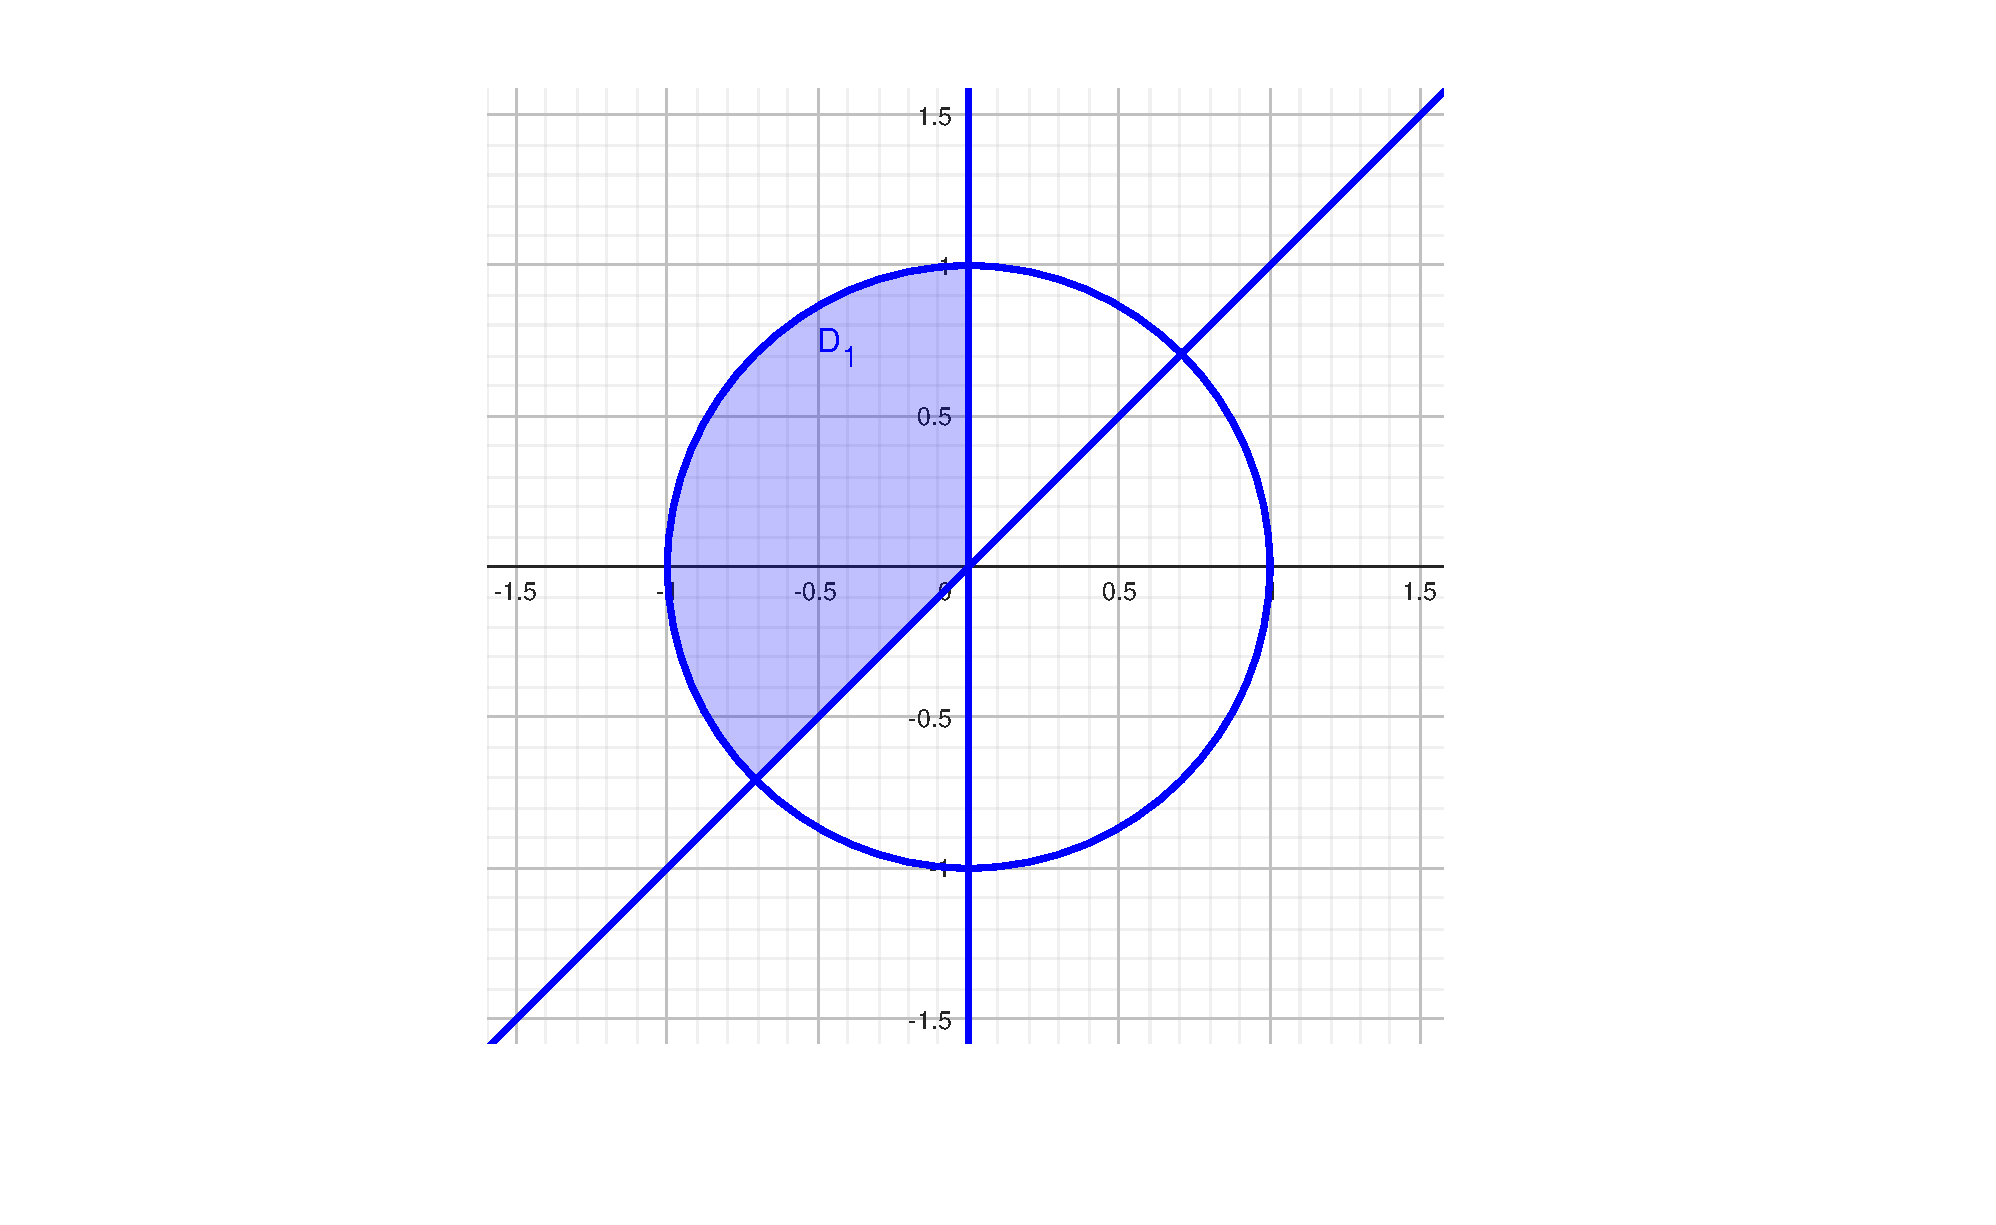
\includegraphics[width=.95\textwidth]{img/grafico-ex6-8.pdf}
		\caption*{Dominio di $D_{1}$, dove $x^{2} + y^{2} \le 1$ identifica una circonferenza, $x \le 0$ identifica la parte di sinistra del piano cartesiano e $y \ge x$ taglia in due per obliquo prendendo la parte superiore.}
	\end{figure}\newpage

	\noindent
	Si continua disegnando il secondo dominio:
	\begin{figure}[!htp]
		\centering
		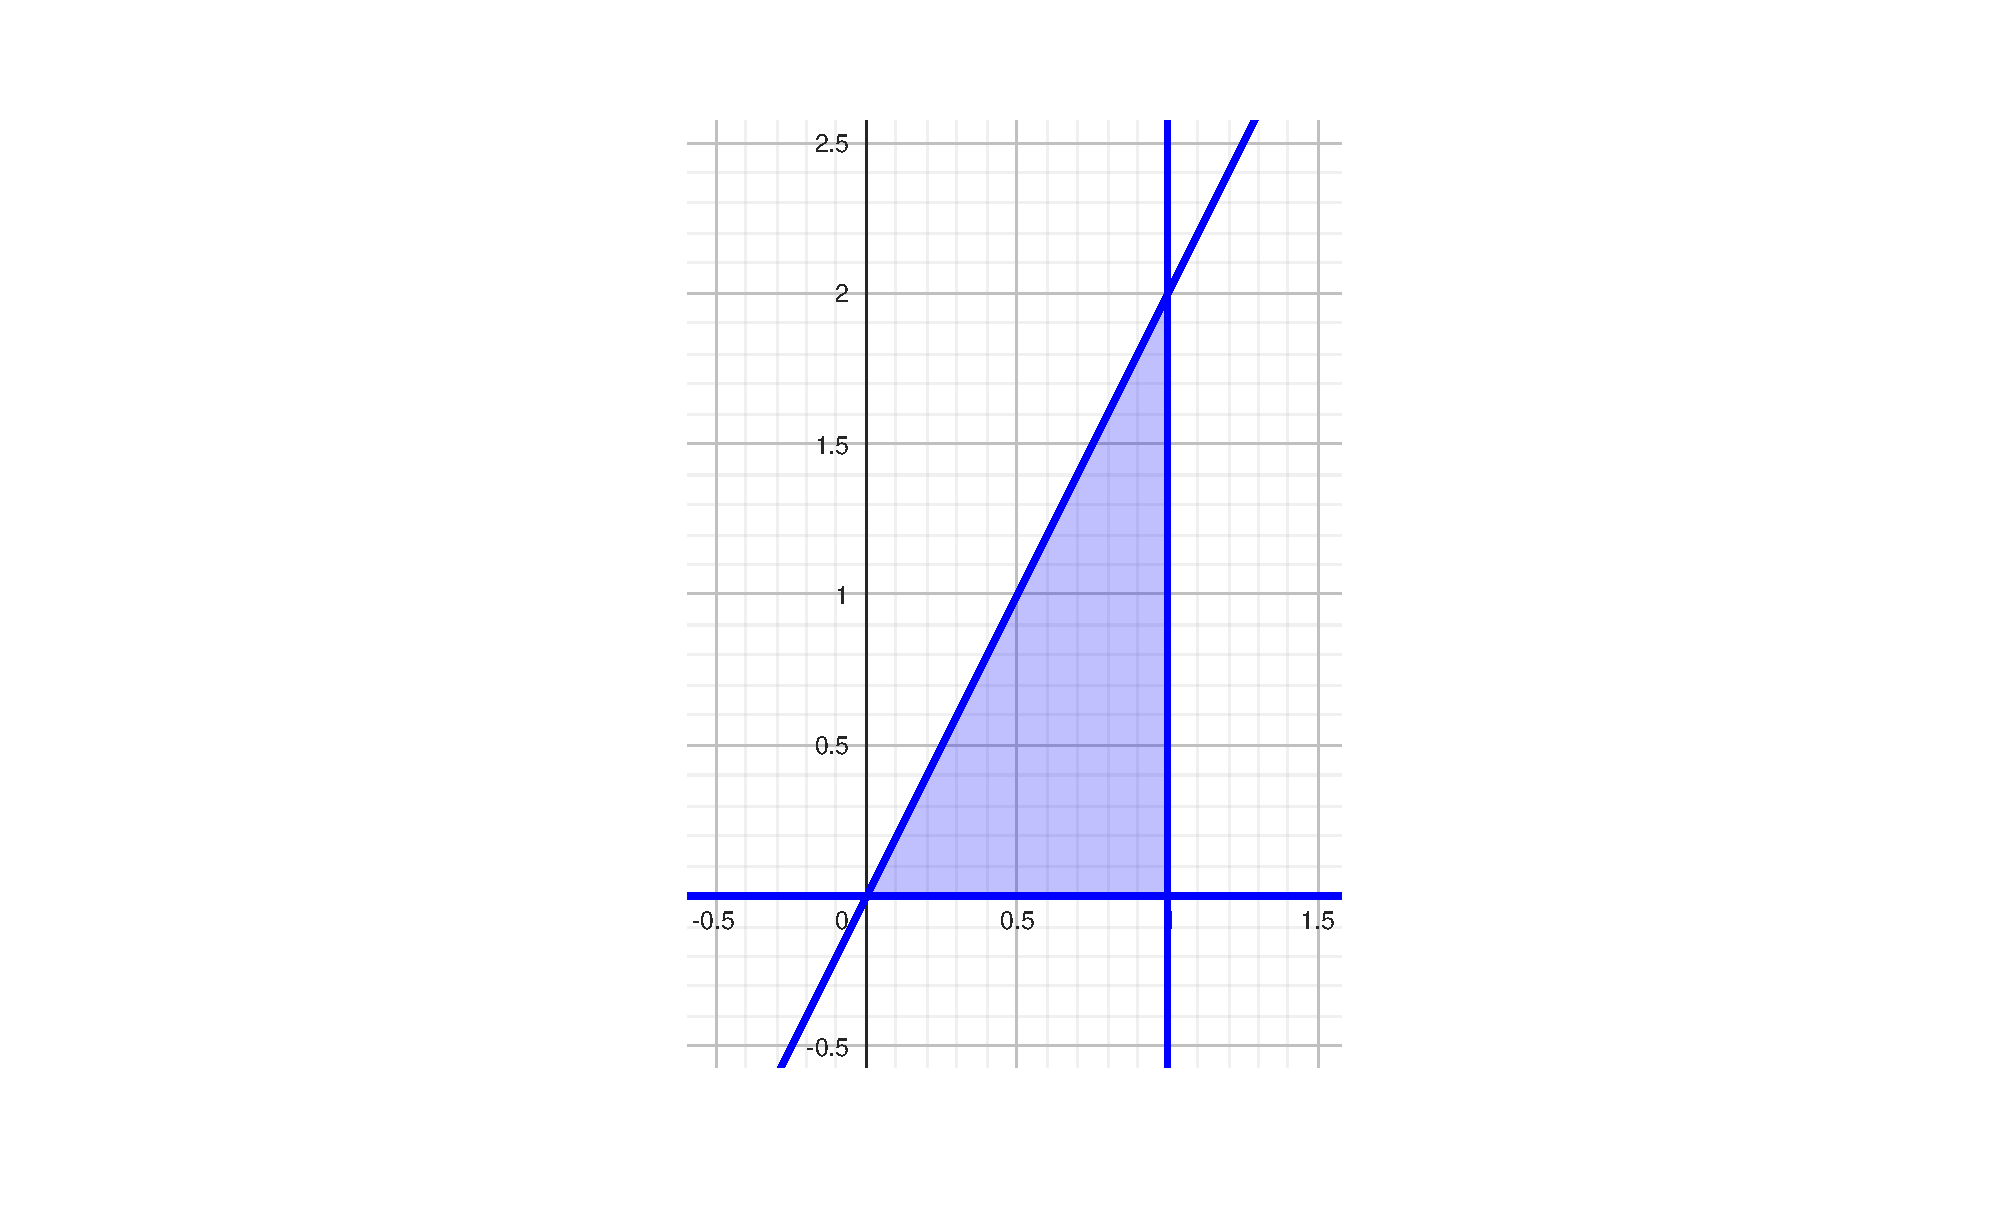
\includegraphics[width=.6\textwidth]{img/grafico-ex6-9.pdf}
		\caption*{Dominio di $D_{2}$, dove $0 \le y \le 2x$ rappresenta la retta obliqua e $x \le 1$ delimita l'area.}
	\end{figure}

	\noindent
	Il \textbf{secondo passo} è la risposta all'esercizio. L'\underline{unione} dei due domini non è altro che la somma di due integrali, ovvero:
	\begin{equation*}
		\displaystyle\underset{D_{1} \cup D_{2}}{\int\hspace{-.5em}\int} xy \: \mathrm{d}x \: \mathrm{d}y = \underset{D_{1}}{\int\hspace{-.5em}\int} xy \: \mathrm{d}x \: \mathrm{d}y + \underset{D_{2}}{\int\hspace{-.5em}\int} xy \: \mathrm{d}x \: \mathrm{d}y
	\end{equation*}
	Quindi, si procede con il loro calcolo.\newline

	\noindent
	Il \textbf{terzo passo} è calcolare gli integrali. Si parte da $D_{1}$ dove è evidente che è necessario proseguire per coordinate polari. Quindi, $\theta$ è compreso tra 90\degree e 225\degree, mentre $\rho$ è compreso tra $0$ (origine) e $1$ (raggio):
	\begin{equation*}
		\begin{array}{rcl}
			1\degree &=& \dfrac{\pi}{180} \\ [1em]
			90\degree &=& \dfrac{90\pi}{180} = \dfrac{\pi}{2} \\ [1em]
			225\degree &=& \dfrac{225\pi}{180} = \dfrac{5\pi}{4}
		\end{array}
	\end{equation*}\newpage

	\noindent
	Si scrivono formalmente le disuguaglianze:
	\begin{gather*}
		\dfrac{\pi}{2} \le \theta \le \dfrac{5\pi}{4} \\
		0 \le \rho \le 1
	\end{gather*}
	Ricordando che:
	\begin{equation*}
		\begin{cases}
			x = \rho \cos\left(\theta\right) \\
			y = \rho \sin\left(\theta\right)
		\end{cases}
	\end{equation*}
	Si risolve l'integrale doppio ricordando di sostituire anche le variabili:
	\begin{equation*}
		\begin{array}{ll}
			=& \displaystyle\int_{\frac{\pi}{2}}^{\frac{5\pi}{4}} \int_{0}^{1} \left(\rho\cos\left(\theta\right)\right) \cdot \left(\rho\sin\left(\theta\right)\right) \cdot \rho \: \mathrm{d}\rho \: \mathrm{d}\theta \\ [1.5em]
			%
			=& \displaystyle\int_{\frac{\pi}{2}}^{\frac{5\pi}{4}} \int_{0}^{1} \rho^{3}\cos\left(\theta\right) \sin\left(\theta\right) \: \mathrm{d}\rho \: \mathrm{d}\theta \\ [1.5em]
			%
			\rightarrow& \text{si portano fuori le costanti} \\ [1em]
			%
			=& \displaystyle\int_{\frac{\pi}{2}}^{\frac{5\pi}{4}} \left(\cos\left(\theta\right) \cdot \sin\left(\theta\right)\right) \cdot \left[\dfrac{\rho^{4}}{4}\right]_{0}^{1} \: \mathrm{d}\theta \\ [1.5em]
			%
			=& \displaystyle\int_{\frac{\pi}{2}}^{\frac{5\pi}{4}} \cos\left(\theta\right) \cdot \sin\left(\theta\right) \cdot \dfrac{1}{4} \: \mathrm{d}\theta \\ [1.5em]
			%
			\rightarrow& \text{si risolve per sostituzione: }\mathrm{d}\theta = \dfrac{1}{t'} \: \mathrm{d}t; \hspace{1em} t = \sin\left(\theta\right); \hspace{1em} t'=\cos\left(\theta\right) \\ [1.5em]
			%
			=& \dfrac{1}{4} \cdot \displaystyle\int_{\frac{\pi}{2}}^{\frac{5\pi}{4}} \cancel{\cos\left(\theta\right)} \cdot t \cdot \dfrac{1}{\cancel{\cos\left(\theta\right)}} \: \mathrm{d}t \\ [1.5em]
			%
			=& \left[\dfrac{1}{4} \cdot \dfrac{t^{2}}{2}\right]_{\frac{\pi}{2}}^{\frac{5\pi}{4}} \\ [1.5em]
			%
			\rightarrow& \text{si reinserisce la variabile originale} \\ [1.5em]
			%
			=& \left[\left(\dfrac{1}{4} \cdot \dfrac{\sin^{2}\left(\dfrac{5\pi}{4}\right)}{2}\right) - \left(\dfrac{1}{4} \cdot \dfrac{\sin^{2}\left(\dfrac{\pi}{2}\right)}{2}\right)\right] \\ [2em]
			%
			=& \left[\left(\dfrac{1}{4} \cdot \dfrac{\frac{1}{2}}{2}\right) - \left(\dfrac{1}{4} \cdot \dfrac{1}{2}\right)\right] \\ [1.5em]
			%
			=& \dfrac{1}{16} - \dfrac{1}{8} \\ [1.5em]
			%
			=& -\dfrac{1}{16}
		\end{array}
	\end{equation*}\newpage

	\noindent
	Adesso si calcola il doppio integrale su $D_{2}$. Guardando il grafico si procede con la risoluzione per $x$-semplice. Quindi, i limiti di $x$ e $y$ saranno:
	\begin{gather*}
		0 \le x \le 1 \\
		0 \le y \le 2x
	\end{gather*}
	La $y$ ha \dquotes{estremi} come valori e la $x$ possiede due funzioni, anche se $1$ è un valore.
	\begin{equation*}
		\begin{array}{ll}
			=& \displaystyle\int_{0}^{1} \int_{0}^{2x} xy \: \mathrm{d}y \: \mathrm{d}x \\ [1.5em]
			%
			=& \displaystyle\int_{0}^{1} x \cdot \int_{0}^{2x} y \: \mathrm{d}y \: \mathrm{d}x \\ [1.5em]
			%
			=& \displaystyle\int_{0}^{1} x \cdot \left[\dfrac{y^{2}}{2}\right]_{0}^{2x} \: \mathrm{d}x \\ [1.5em]
			%
			=& \displaystyle\int_{0}^{1} x \cdot \left[\dfrac{4x^{2}}{2} - \dfrac{0^{2}}{2}\right] \: \mathrm{d}x \\ [1.5em]
			%
			=& \displaystyle\int_{0}^{1} 2x^{3} \: \mathrm{d}x \\ [1.5em]
			%
			=& \left[\dfrac{x^{4}}{2}\right]_{0}^{1} \\ [1.5em]
			%
			=& \left[\left(\dfrac{1}{2}\right) - \left(\dfrac{0^{4}}{2}\right)\right] \\ [1.5em]
			%
			=& \dfrac{1}{2}
		\end{array}
	\end{equation*}
	Il \textbf{quarto e ultimo passo} è sommare i due integrali trovati:
	\begin{equation*}
		\begin{array}{rcl}
			\displaystyle\underset{D_{1} \cup D_{2}}{\int\hspace{-.5em}\int} xy \: \mathrm{d}x \: \mathrm{d}y &=& \underset{D_{1}}{\displaystyle\int\hspace{-.5em}\int} xy \: \mathrm{d}x \: \mathrm{d}y + \underset{D_{2}}{\displaystyle\int\hspace{-.5em}\int} xy \: \mathrm{d}x \: \mathrm{d}y \\ [1.5em]
			&=& -\dfrac{1}{16} + \dfrac{1}{2} \\ [1.5em]
			&=& \dfrac{7}{16}
		\end{array}
	\end{equation*}
	
	\newpage
	\subsubsection{Integrali doppi e calcolo del baricentro}

	Un'integrazione doppia può essere ancora più complessa se viene dato un grafico, alcuni punti e viene richiesto di calcolare il baricentro del dominio. L'esame del 03/03/2023 era il seguente: \textcolor{Green4}{\textbf{\emph{Sia $D$ la regione del piano limitata dalla curva $y = -\sqrt[3]{4x}$, dal segmento che unisce i punti $\left(-1,0\right)$ e $\left(-2,2\right)$ e dall'asse $x$ (vedi figura).}}}
	\begin{figure}[!htp]
		\centering
		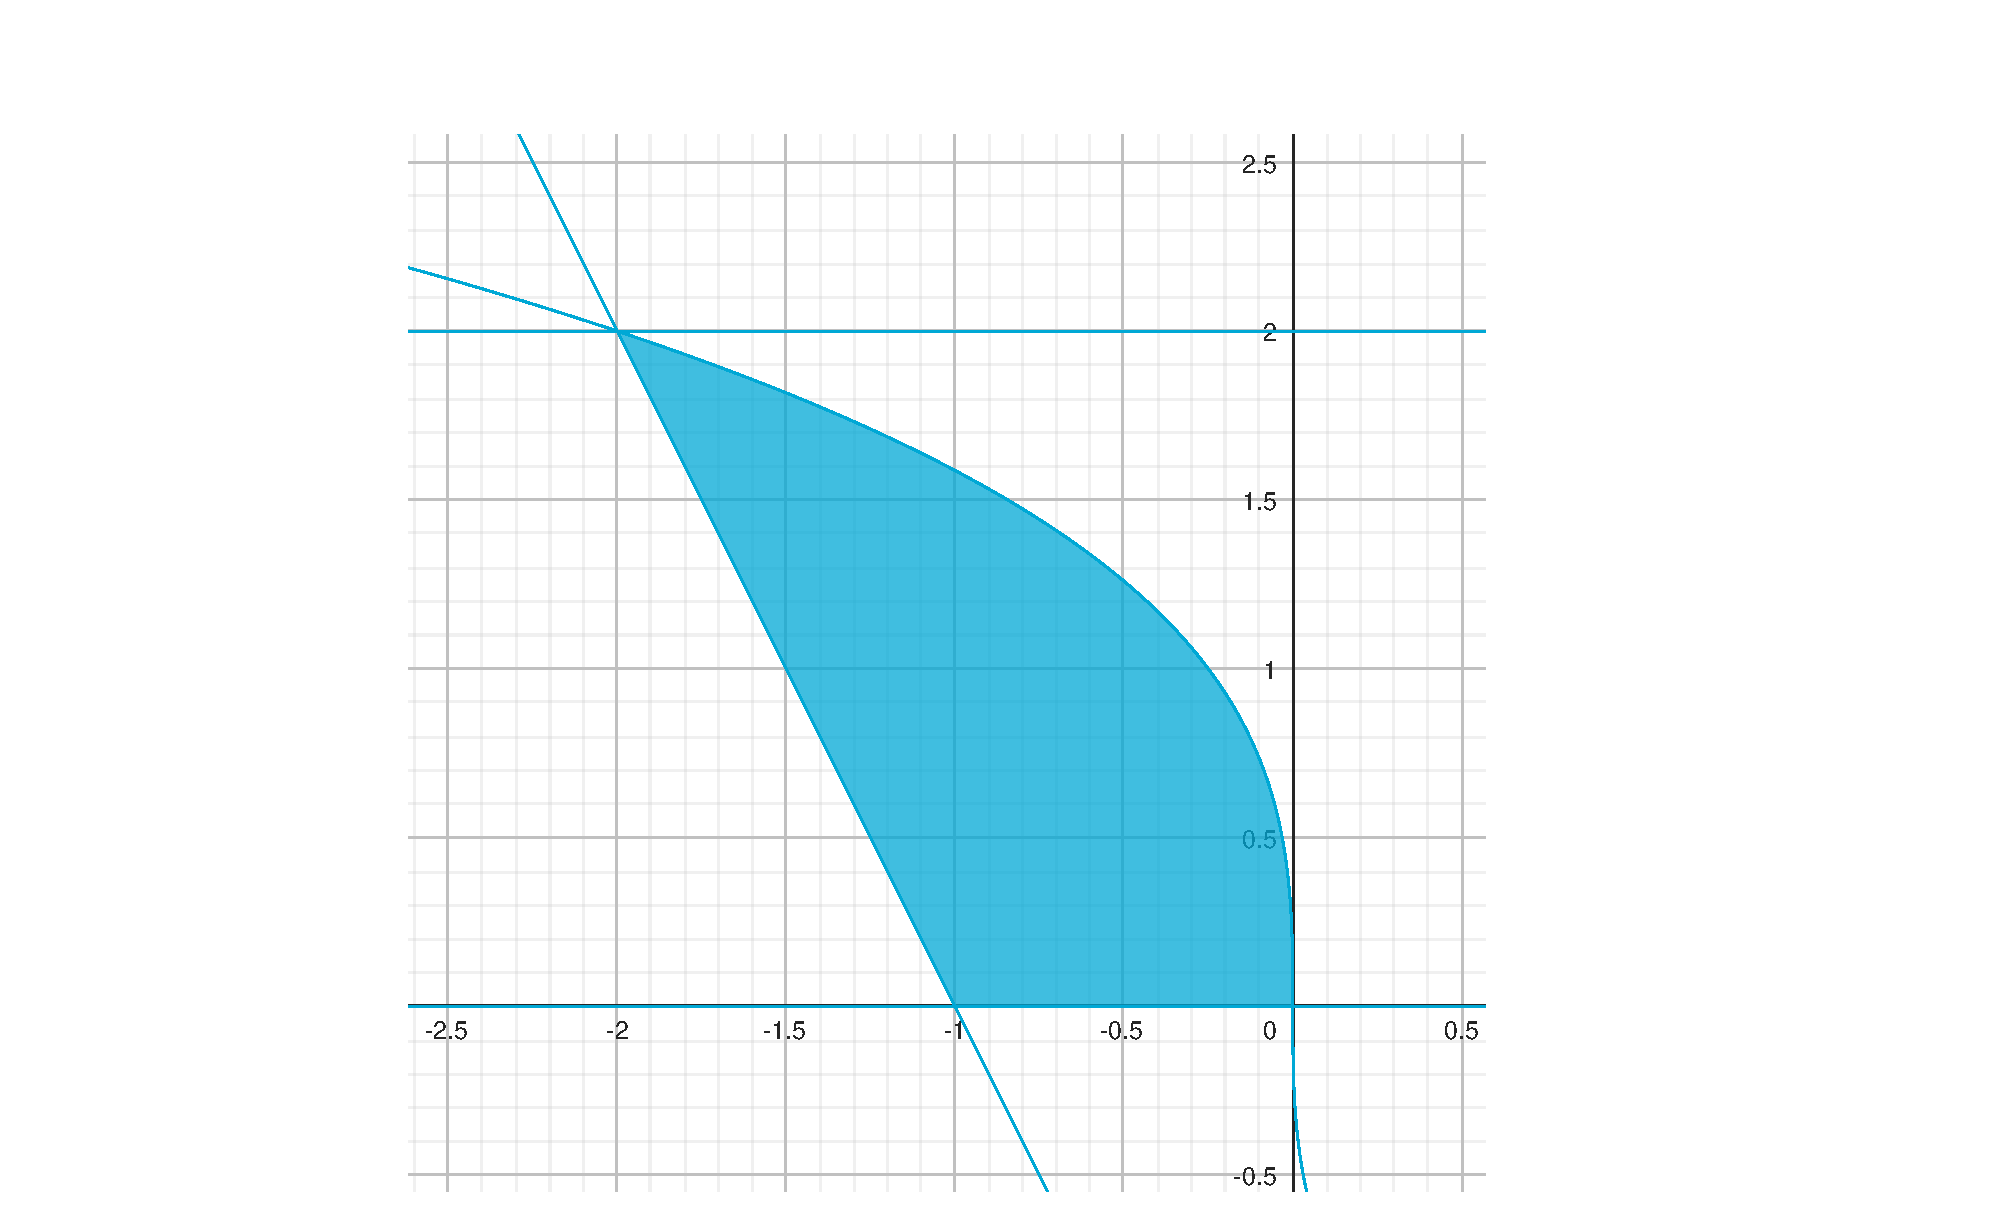
\includegraphics[width=.8\textwidth]{img/grafico-ex6-10.pdf}
	\end{figure}

	\noindent
	\textcolor{Green4}{\textbf{\emph{Calcolare}} $\displaystyle\int\int_{D} y \: \mathrm{d}x \: \mathrm{d}y$}\newline
	\textcolor{Green4}{\textbf{\emph{Sapendo che l'area della regione $D$ è $2$, determinare la quota $y$ del baricentro di $D$.}}}\newline

	\noindent
	Si elencano qua di seguito i passaggi da fare prima di arrivare a calcolare il baricentro. Si noti bene che lo svolgimento è identico a quello applicato nei precedenti capitoli:
	\begin{enumerate}
		\item Si calcola l'equazione della retta passante per i due punti $\left(-1,0\right)$ e $\left(-2,2\right)$ con la formula $\dfrac{x-x_{1}}{x_{2}-x_{1}} = \dfrac{y-y_{1}}{y_{2}-y_{1}}$;

		\item Si ragiona su come calcolare l'integrale doppio. In questo caso, conviene utilizzare il calcolo per $y$-semplice. Quindi, si esplicita la $y$ nell'equazione della curva data dall'esercizio;

		\item Si svolge l'integrale dopo aver calcolato gli estremi di integrazione: $0 \le y \le 2$, $-\frac{1}{2}y-1 \le x \le -\frac{y^{3}}{4}$;
	\end{enumerate}
	Per calcolare il \textbf{baricentro}, si utilizza la seguente formula:
	\begin{equation*}
		y_{G} = \dfrac{\displaystyle\int\int_{D} y \: \mathrm{d}x \: \mathrm{d}y}{area\left(D\right)}
	\end{equation*}
	Anche se non è questo il caso, se fosse stato chiesto di calcolare il baricentro in $x$, sarebbe cambiato solo l'integrale:
	\begin{equation*}
		x_{G} = \dfrac{\displaystyle\int\int_{D} x \: \mathrm{d}x \: \mathrm{d}y}{area\left(D\right)}
	\end{equation*}
\end{document}